%% get rid of autoindent   :setl noai nocin nosi inde=
%%
%% 1. pdflatex main
%% 2. bibtex main
%% 3. pdflatex main
%% 3. pdflatex main
%\documentclass[review]{elsarticle}
\documentclass[]{article}
%\documentclass[preprint]{elsarticle}

\usepackage{lineno,hyperref}
\modulolinenumbers[5]

\usepackage[fleqn]{amsmath} 
\usepackage{amssymb}
\usepackage{graphicx}
\usepackage{tabularx} 
\usepackage{footnote}
\usepackage{titlesec}
\titleformat{\section}{\large\bfseries}{\thesection}{1em}{}

\makesavenoteenv{tabular}
\makesavenoteenv{table}
\usepackage[percent]{overpic}
\usepackage{subfigure}% subcaptions for subfigures
\usepackage{subfigmat}% matrices of similar subfigures, aka small multiples
\usepackage{array}
\setlength{\mathindent}{0pt}

\renewcommand{\labelitemi}{$\triangleright$}
\renewcommand{\labelitemii}{$\triangleright$}
\renewcommand{\labelitemiii}{$\triangleright$}
\renewcommand{\labelitemiv}{$\triangleright$}


%\journal{Journal of Computational Physics}

\newcommand{\mb}{\mathbf}
\newcommand{\tn}{\textnormal}
\newcommand{\unit}[1]{\ensuremath{\, \mathrm{#1}}}

\newcommand{\bmz}{\mbox{\boldmath $z$\unboldmath}}
\newcommand{\bmr}{\mbox{\boldmath $r$\unboldmath}}
\newcommand{\bmb}{\mbox{\boldmath $b$\unboldmath}}
\newcommand{\bms}{\mbox{\boldmath $s$\unboldmath}}
\newcommand{\bmg}{\mbox{\boldmath $g$\unboldmath}}
\newcommand{\bmq}{\mbox{\boldmath $q$\unboldmath}}
\newcommand{\bmU}{\mbox{\boldmath $U$\unboldmath}}
\newcommand{\bmu}{\mbox{\boldmath $u$\unboldmath}}
\newcommand{\bmv}{\mbox{\boldmath $v$\unboldmath}}
\newcommand{\bmw}{\mbox{\boldmath $w$\unboldmath}}
\newcommand{\bmm}{\mbox{\boldmath $m$\unboldmath}}
\newcommand{\bmi}{\mbox{\boldmath $i$\unboldmath}}
\newcommand{\bmj}{\mbox{\boldmath $j$\unboldmath}}
\newcommand{\bmk}{\mbox{\boldmath $k$\unboldmath}}
\newcommand{\bmx}{\mbox{\boldmath $x$\unboldmath}}
\newcommand{\bmX}{\mbox{\boldmath $X$\unboldmath}}
\newcommand{\bmH}{\mbox{\boldmath $H$\unboldmath}}
\newcommand{\bmy}{\mbox{\boldmath $y$\unboldmath}}
\newcommand{\bmn}{\mbox{\boldmath $n$\unboldmath}}
\newcommand{\bmf}{\mbox{\boldmath $f$\unboldmath}}
\newcommand{\bmF}{\mbox{\boldmath $F$\unboldmath}}
\newcommand{\bmS}{\mbox{\boldmath $S$\unboldmath}}
\newcommand{\bmG}{\mbox{\boldmath $G$\unboldmath}}
\newcommand{\bmV}{\mbox{\boldmath $V$\unboldmath}}
\newcommand{\bmI}{\mbox{\boldmath $I$\unboldmath}}
\newcommand{\bmD}{\mbox{\boldmath $D$\unboldmath}}
\newcommand{\bmnu}{\mbox{\boldmath $\nu$\unboldmath}}

\newcommand{\DefTen}{\mathbb{D}}
\newcommand{\EyeTen}{\mathbb{I}}

\DeclareMathOperator{\Ei}{Ei}

\newcommand{\MVBcmnt}[1]{{\color{red}{\em #1}}}

\newcolumntype{L}[1]{>{\raggedright\let\newline\\\arraybackslash\hspace{0pt}}m{#1}}
\newcolumntype{C}[1]{>{\centering\let\newline\\\arraybackslash\hspace{0pt}}m{#1}}
\newcolumntype{R}[1]{>{\raggedleft\let\newline\\\arraybackslash\hspace{0pt}}m{#1}}

%%\bibliographystyle{elsarticle-num}
\bibliographystyle{acm}
%%%%%%%%%%%%%%%%%%%%%%%

\title{An improved 
  coupled level set and continuous moment-of-fluid method 
  for simulating multiphase flows with phase change
  \thanks{this material is based upon work supported by National
   Aeronautics and Space Administration under grant number
   80NSSC20K0352}}

%%!!format authors properly
%\author{
%	LastName1, FirstName1\\
%	\texttt{first1.last1@xxxxx.com}
%	\and
%	LastName2, FirstName2\\
%	\texttt{first2.last2@xxxxx.com}
%}
\author{
  Ye, Zhouteng \\
  ZJUI Institute, Zhejiang University, Haining, China
  \and
  Estebe, Cody \\
  Dept. of math, FL State Univ. 
  \and
  Liu, Yang \\
  Dept. of Mech. Engr., FL State Univ.
  \and
  Vahab, Mehdi \\
  Mech. and Aero. Engr. Mathworks, Natick, MA
  \and
  Huang, Zeyu \\
  School of Aerospace Engineering, Tsinghua University
  \and
  Sussman, Mark \\
  Dept. of math, FL State Univ. 
  \and
  Moradikazerouni, Alireza \\
  Dept. of Mech. Engr., FL State Univ.
  \and
  Shoele, Kourosh  \\
  Dept. of Mech. Engr., FL State Univ.
  \and
  Lian, Yongsheng \\
  Dept. of Mech. Engr., U. of Louisville
  \and
  Ohta, Mitsuhiro \\
  Dept. of Mech. Sci, Tokushima University 
  \and
  Hussaini, M. Yousuff \\ 
  Dept. of math, FL State Univ. 
}

\begin{document}
\maketitle

ABSTRACT:
An improved algorithm for computing multiphase flows is presented in which the multimaterial Moment-Of-Fluid (MOF) algorithm for multiphase flows, initially described by Li et al (2015), is enhanced addressing existing MOF difficulties in computing solutions to problems in which surface tension forces are crucial for understanding salient flow mechanisms.  The Continuous Moment of Fluid (CMOF) method is motivated in this article.  The CMOF reconstruction method inherently removes the ``checkerboard instability'' that persists when using the MOF method on surface tension driven multiphase (multimaterial) flows.  The CMOF reconstruction algorithm is accelerated by coupling the CMOF method to the level set method and coupling the CMOF method to a Decision Tree machine learning algorithm.

Multiphase flow examples are shown in 2D, 3D axisymmetric ``RZ,'' and 3D coordinate systems.  Examples include two material and three material multiphase flows: bubble formation, the impingement of a liquid jet on a gas bubble in a cryogenic fuel tank, freezing, and liquid lens dynamics.
% Fred Stern -> reconstructed distance function coupled with VOF 
%%cite: Mukundan
\linenumbers
\section{Introduction}
We present an improved ``Continuous Moment-of-Fluid'' (CMOF) algorithm
for computing solutions to multiphase (multimaterial) flows.  We 
demonstrate the benefits of our new algorithm, beyond that of the 
current state-of-the-art, on these benchmark multiphase flow
problems:
bubble formation\cite{helsby1955behaviour} (see Section \ref{bubform}),
freezing\cite{hu2010icing} (see Section \ref{freezing_sec}), 
liquid lens\cite{MIAO2021109358} (see Section \ref{liqlens}),
and bubble dynamics in a Cryogenic fuel 
tank\cite{bentz1993low} (see Section \ref{TPCEsec}).

Figure \ref{checkerboard} (LEFT figure) 
illustrates the 
Moment-of-Fluid\cite{dyadechko2005moment,ahn2007multi,ahn2009adaptive}
reconstruction of a ``saw tooth'' function that has a wave
length of $\Delta x$.  The MOF reconstruction is very ``noisy'' in the
sense that the highest frequency
Fourier coefficients of the discrete Fourier transform
of the reconstruction do not decay with repeated reconstructions.
In other-words the amplitudes of the high frequency Fourier modes may
not decay when exposed to the repeated process of
(1) MOF advection, and (2) MOF reconstruction.
The presence of $O(\Delta x)$ wave length noise is
a problem for applications involving  
surface tension driven flows.  Standard
Volume-of-Fluid techniques for extracting the curvature
from volume fractions\cite{sussman2003second,cummins2005estimating}
will extract a zero curvature from a ``saw tooth'' interface 
since the associated volume fraction field {\em and} centroid
field varies in the $y$
direction only.  In other words, the
underlying computational fluid dynamics surface tension force
algorithm will never ``see'' the jagged interface and therefore will have
no way for removing the noise.  If there is viscosity, the presence of the 
noise is unphysical and the noise can lead to collateral damage (see Figure 
\ref{MOF_liquid_lens} and Table \ref{liquidlens_table}) 
to the overall flow field; the noise can
result in loss of accuracy.

In order to overcome the ``MOF checkerboard instability'' issue, we have 
developed the ``Continuous Moment of Fluid'' (CMOF) interface reconstruction
algorithm\cite{VAHAB2021}.  
Referring to Figure \ref{checkerboard}, the repeated process
of (1) CMOF advection, followed by (2) CMOF reconstruction, 
will quickly eliminate the
noise.  The difference between CMOF and MOF is that in the CMOF algorithm,
the reference centroid is the material centroid relative to the 
encompassing $3\times 3\times 3$ stencil of grids cells, rather than just the
center cell.  See Figure \ref{CMOFcentroid}.   

We remark that alternative approaches to using MOF for multiphase 
(multimaterial)
flows, e.g the level set 
method\cite{smith2002projection,shetabivash2020multiple,starinshak2014new}, 
phase field method\cite{HUANG2022110795}, 
front tracking method \cite{vu2015numerical},
or standard ``PLIC'' VOF 
methods\cite{ancellin2022extension,schofield2008material,schofield2009second}, 
do not have the
``MOF checkerboard instability'' problem.  These alternative approaches
have other difficulties.  The level set or front tracking
multimaterial 
approaches\cite{smith2002projection,shetabivash2020multiple,starinshak2014new,vu2015numerical} 
are not volume preserving methods.  
The phase field method\cite{HUANG2022110795} 
smears the interface over 3 grid
cells or more.  The standard, second order, ``PLIC'' VOF methods for 
$M$ material multimaterial 
flows\cite{ancellin2022extension,schofield2008material,schofield2009second} 
minimize a cost function which has $27(M-1)$ 
degrees of freedom; i.e. the control variable space 
is $27(M-1)$ dimensions.

Our improved CMOF method, on the other-hand, admits a sharp reconstructed
interface, is volume preserving, and the control variable space has only
$3(M-1)$ dimensions.  The CMOF reconstruction algorithm has been 
improved in this article by applying ``Decision Tree'' 
machine learning techniques 
in order to rapidly determine the optimal ``CMOF'' slope.
We choose the Decision Tree algorithm\cite{breiman1984classification} which is 
a ``lossless'' method if one chooses to store all of the training
data samples in the tree structure.  
In Table \ref{tab:triple_point}, we summarize the
existing state-of-the-art for numerical methods for 
multiphase (multimaterial)
flows with surface tension.

\begin{table}[htbp]
  \centering
  \scalebox{0.7}
  {
  \begin{tabular}[h]{|C{2cm}|C{2cm}|C{2cm}|C{2cm}|C{2cm}|C{2cm}|C{2cm}|}
    \hline
    Author(s) & 
    Triple point\newline reconstruction\newline algorithm\newline DOF$^{1}$ &
    Coupled\newline with fluid &
    Volume\newline preserving &
    Sharp\newline interface & 
    Curvature\newline discretization \\
    \hline
    Smith et al.~\cite{smith2002projection} & Level set & Yes & No  & Yes & Level set \\ \hline
    Ahn and Shahkov\cite{ahn2007multi} & $\tn{VOF-GRAD}^2$\newline $\tn{VOF-LVIRA}^3$ \newline MOF 
                 \newline 27 or 3 $\times(M-1)$& No & Yes & Yes & N/A\\ \hline
    Kim\cite{kim2007phase} & Phase field & Yes & Yes & No & Phase field \\ \hline
    Dyadechko and Shashkov\cite{dyadechko2008reconstruction} & MOF \newline $3(M-1)$ & No & Yes & Yes & N/A \\ \hline
    Caboussat et al.~\cite{caboussat2008numerical} & $\tn{VOF-IP}^4$ \newline $27(M-1)$ & Yes & No & Yes & 
                                           Convolution/Height function\cite{francois2006balanced}\\ \hline
    Schofield et al.~\cite{schofield2008material, schofield2009second} & $\tn{VOF-PD}^5$ \newline $27(M-1)$ 
	                                         & No & Yes & Yes & N/A \\ \hline
    Sijoy and Chaturvedi\cite{sijoy2010volume} & $\tn{VOF-PLIC}^6$ \newline $27(M-1)$& 
	                                      Yes & Yes & Yes & N/A \\ \hline
    Kucharik et al.~\cite{kucharik2010comparative} & VOF-PLIC \newline VOF-PD \newline MOF \newline 27 or 3 $\times(M-1)$ &
	                                         Yes & Yes & Yes & N/A \\ \hline
    Bonhomme et al.~\cite{bonhomme2012inertial} & VOF \newline $27(M-1)$ & Yes & Yes & No & VOF \\ \hline
    Starinshak et al.~\cite{starinshak2014new} & Interface level set & Yes & No & Yes & N/A \\ \hline
    Vu et al.~\cite{vu2015numerical} & Front tracking & Yes & No & Yes & Front tracking \\ \hline
    Pathak and Raessi\cite{pathak2016three} & VOF-PLIC \newline $27(M-1)$ & No & Yes & Yes & N/A \\ \hline
    Shetabivash et al.~\cite{shetabivash2020multiple} & Level Set & Yes & No & Yes & Finite Difference \\ \hline
    Ancellin et al.~\cite{ancellin2022extension} & VOF-PLIC \newline $27(M-1)$ & No & Yes & Yes & N/A \\ \hline
    Huang et al.~\cite{HUANG2022110795} & Phase field & Yes & Yes & No & Phase field \\ \hline
    Present Article, Ye et al & CMOF$^7$ \newline $3(M-1)$ & Yes & Yes & Yes & VOF Height function \\ \hline
  \end{tabular}
  }
 \scalebox{0.7}
 {
 \begin{minipage}{\textwidth}
   $^1$: Degrees of Freedom for 3D reconstruction; $M$ is the number of materials \\
   $^2$: Gradient based interface reconstruction\\
   $^3$: Least squares volume-of-fluid interface reconstruction algorithm\\
   $^4$: Interior-point method for the localization of the triple point\\
   $^5$: Power diagram\\
   $^6$: Piecewise linear interface construction\\
   $^7$: Continuous Moment of Fluid construction\\
   \end{minipage}
 }

\caption{Recent numerical methods of flows with triple points in 
  chronological order.  \label{tab:triple_point} }
\end{table}

\begin{figure}[htbp]
\centering
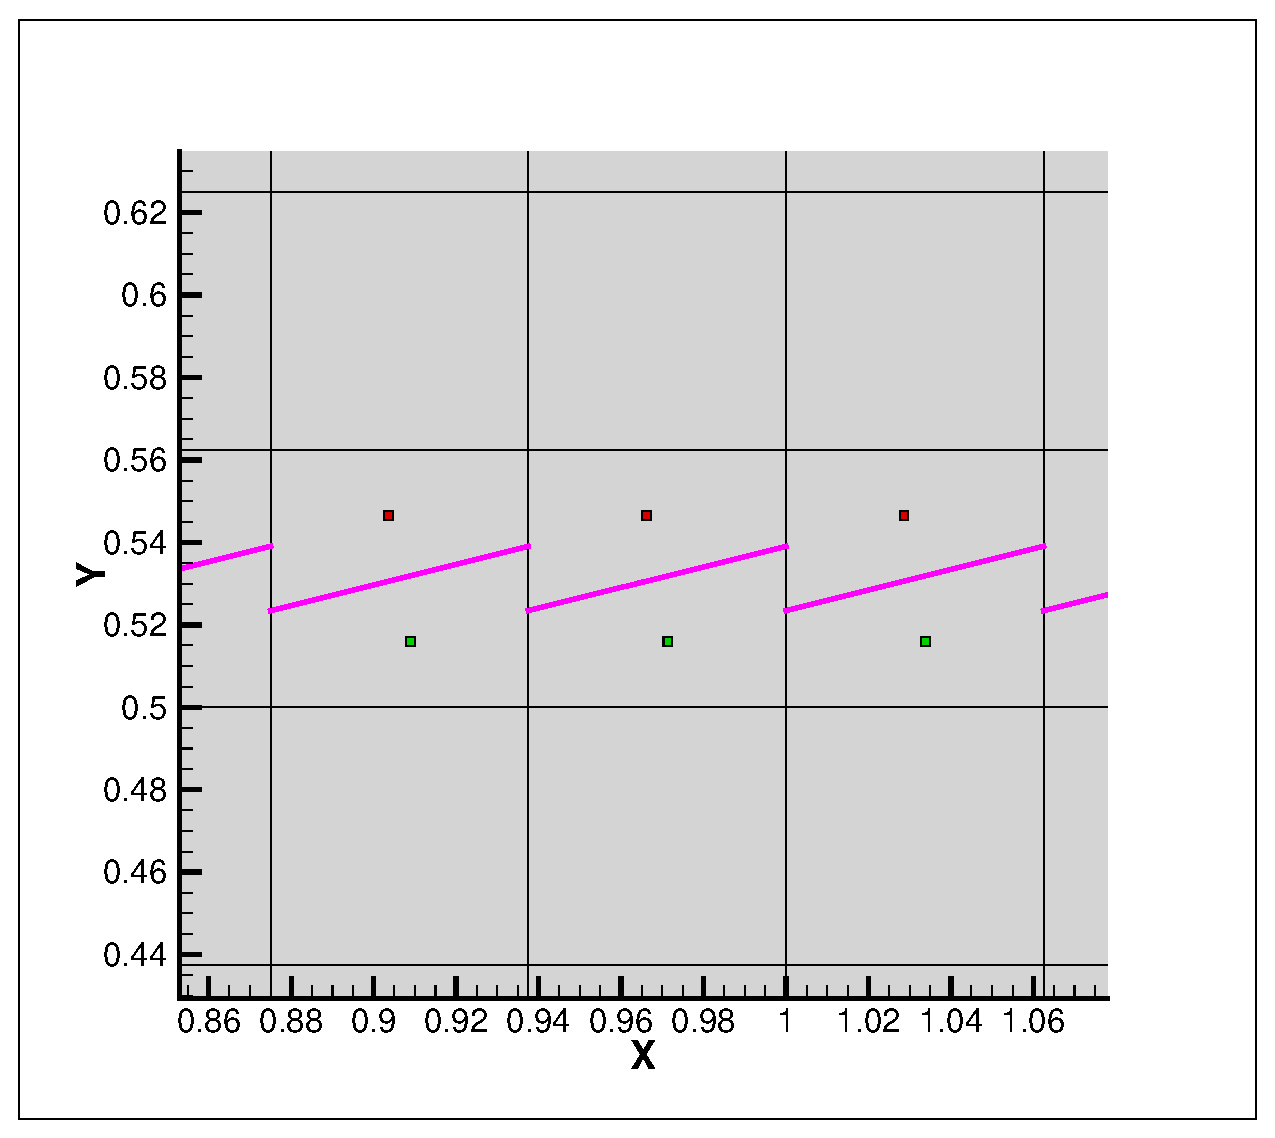
\includegraphics[width=0.4\textwidth]{checkerboardMOF.eps}
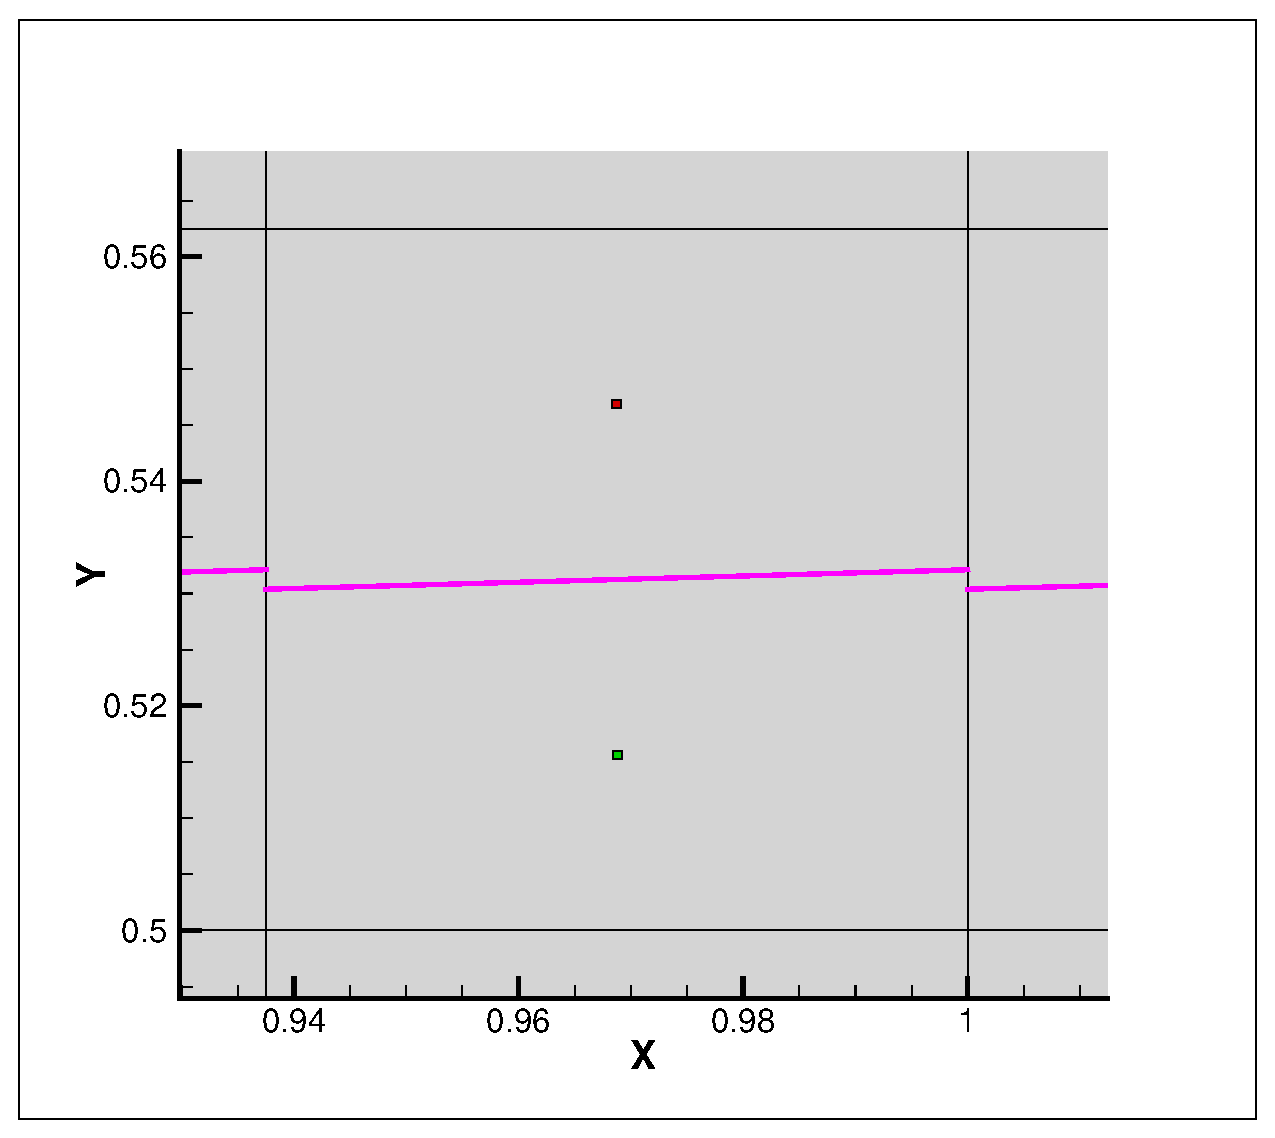
\includegraphics[width=0.4\textwidth]{checkerboardCMOF.eps}
%%REMMERSWAAL and Veldman's parabolic reconstruction WILL NOT SEE
%%the checkerboard pattern (even though they take both F and x into
%%account).
\caption{LEFT:
 Standard curvature discretization methods 
 \cite{sussman2003second,cummins2005estimating,REMMERSWAAL2022111473}
 will predict zero curvature for this saw-tooth
 interface since the volume fractions {\em and} 
 centroids vary only
 in the $y$ direction.  Repeated Moment-of-Fluid (MOF)
 (i) reconstruction followed by (ii) the replacement of the reference
 centroid with the MOF actual centroid will not alter the initial interface
 (ignoring round-off error).  RIGHT: the gaps in the initial saw-tooth 
 interface are reduced by at least a factor of 3 after a single replacement
 of the reference centroid with the CMOF actual centroid.
 \label{checkerboard} }
\end{figure}

\begin{figure}[htbp]
\centering
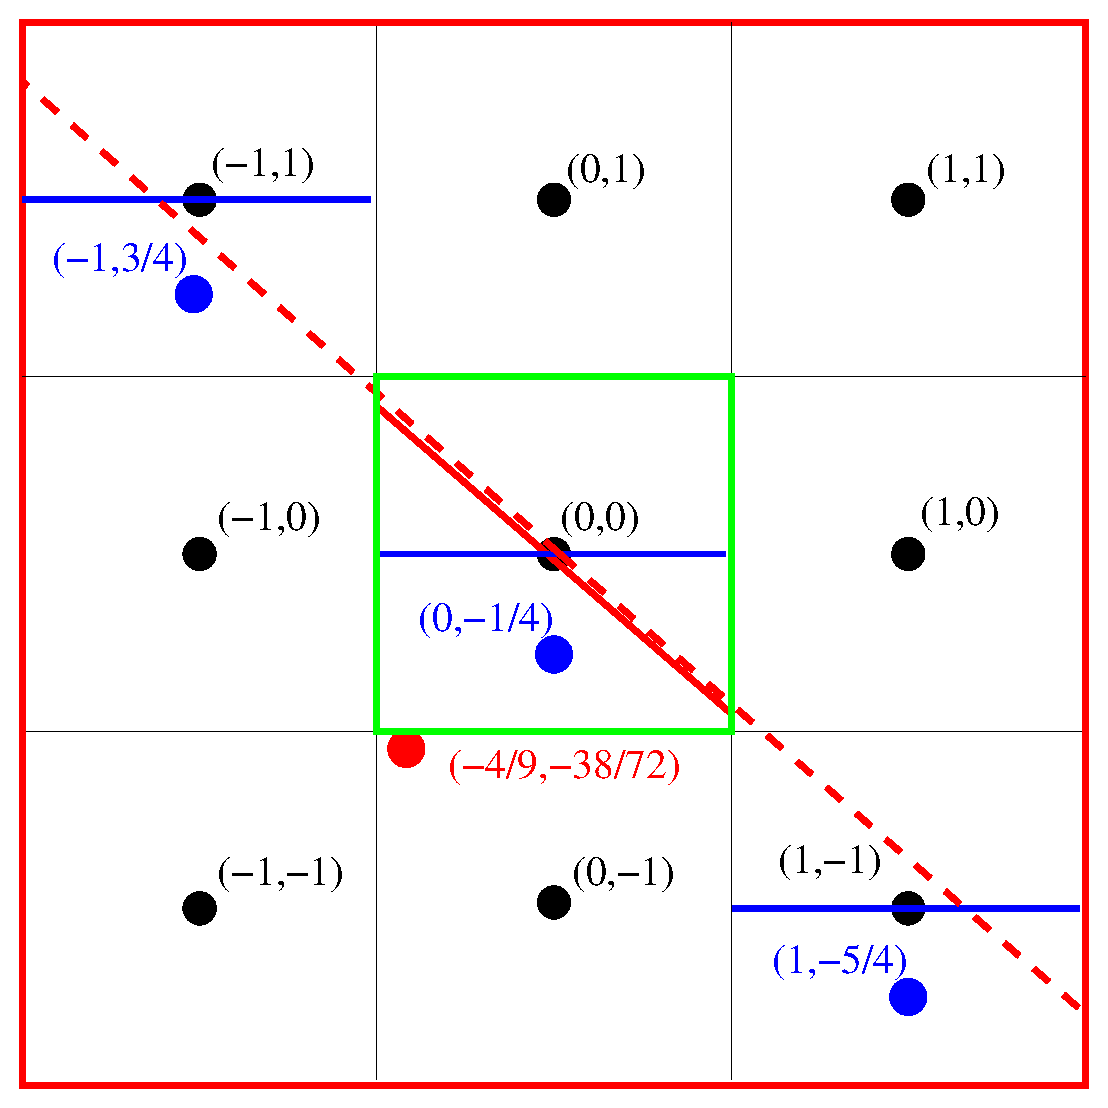
\includegraphics[width=0.8\textwidth]{CMOFcentroid.eps}
\caption{
 Illustration of the difference between Continuous
 Moment-of-Fluid (CMOF) and Moment-of-Fluid (MOF) reconstruction.
 The black circles represent cell centroids, blue circles represent 
 ``material 1'' centroids, and the red circle represents the ``CMOF''
 centroid associated with the center cell (in green) and calculated using
 the $3\times 3$ data surrounded by the CMOF cell (in red).  The CMOF
 reconstructed interface (the red line in the center cell) is the line
 segment which minimizes the difference between the CMOF reference 
 centroid (red circle) and the CMOF derived centroid (centroid associated
 with the dashed red line) subject to the constraint that
 the reference MOF volume fraction (material 1 volume fraction in the 
 center cell) equals the actual CMOF reconstructed
 volume fraction which is the material 1 volume
 fraction below the solid red line in the center cell.
 \label{CMOFcentroid} }
\end{figure}

\section{Background - deforming boundary problems in fluid mechanics}

In the Introduction, we briefly demonstrate the benefits of our
new method over the current state-of-the-art numerical methods
for multi-phase flows in which surface tension forces are important.  
In this section, we give an overview of numerical methods for 
deforming boundary problems in computational fluid dynamics in general,
and show where our new method fits in.

For many deforming boundary problems in fluid dynamics, ``shock capturing''
numerical methods are 
sufficient\cite{godunov1959finite,colella1984piecewise,van1979towards,harten1997high,shu1988efficient,saurel1999multiphase}. Shock capturing methods
have limitations.  According to 
``Godunov's theorem''\cite{godunov1954different}, linear one-step second
order accurate numerical methods for $\phi_{t}+c\phi_{x}=0$ cannot be
monotonicity preserving unless $|c|\Delta t/\Delta x$ is an 
integer.  The concept of ``monotonicity preserving'' methods and its
association to TVD (Total Variational Diminishing) methods was first 
drawn by Harten\cite{harten1997high} who proved that (a) A monotone
scheme is TVD and (b) a TVD scheme is monotonicity preserving.  
When Harten's theory is taken together with Godunov's theorem, one can
see that ``linear'' second order TVD methods only exist under
specialized situations.  Harten's and Godunov's theory are manifested by the
fact that stable shock capturing methods will invariably smear 
discontinuities over time.  

In order to overcome the limitations of shock capturing methods, researchers
have developed (i) front tracking 
methods\cite{glimm1981front,unverdi1992front},
(ii) front capturing 
methods\cite{markstein1951interaction,osher1988fronts,sussman1994level,hirt1981volume,brackbill1992continuum,ahn2007multi,ahn2009adaptive,olsson2005conservative,QiuETALPINNPHASEFIELD2022,
huang2020consistent}, and
(iii) shock fitting methods\cite{SalasShockfitting1976}.

The above methods for overcoming the
the time dependent 
``interface smearing'' problem of the shock capturing methods, have been
further improved by way of hybridization:
the particle level set method\cite{enright2002hybrid},
the hybrid front tracking and level set method\cite{shin2009hybrid},
the coupled level set and volume of fluid method\cite{sussman2000coupled},
and the coupled level set and moment of fluid 
method\cite{ASURIMUKUNDAN2022110864,jemison2013coupled}.

The numerical method that we introduce in this article falls in the latter
``hybrid'' category in which we introduce the hybrid level set and 
Continuous Moment of Fluid (CMOF) method for multiphase/multimaterial
flows.  The level set method and the continuous moment-of-fluid method
are hybridized as follows:
(a) the smooth level set distance function representation is used
to provide an initial guess for the CMOF slope reconstruction
step (see Figure \ref{distancefunction} and Section \ref{MOF_vs_CMOF_sec}),
and (b) the level set distance functions are in turn replaced by the
exact signed distance to the continuous moment-of-fluid reconstructed
interface (see Figure \ref{distancefunction} and 
Section \ref{MMRECON}).  The level set and CMOF representations are 
synchronized every time step.

\begin{figure}[htbp]
  \centering
    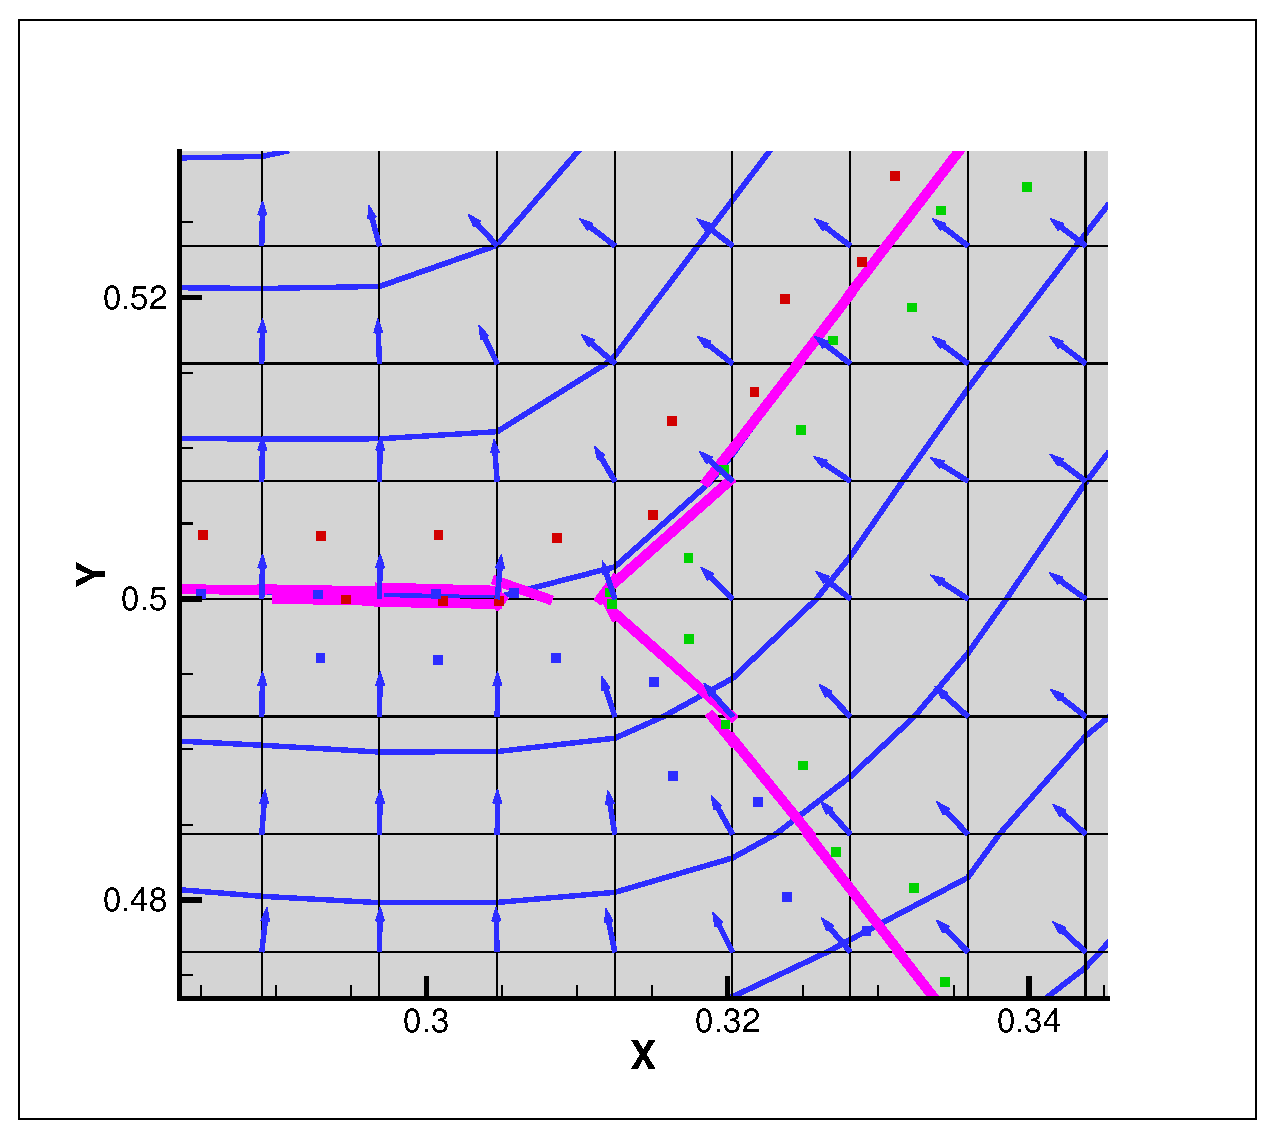
\includegraphics[width=0.45\textwidth]{zoomed_in.eps}
    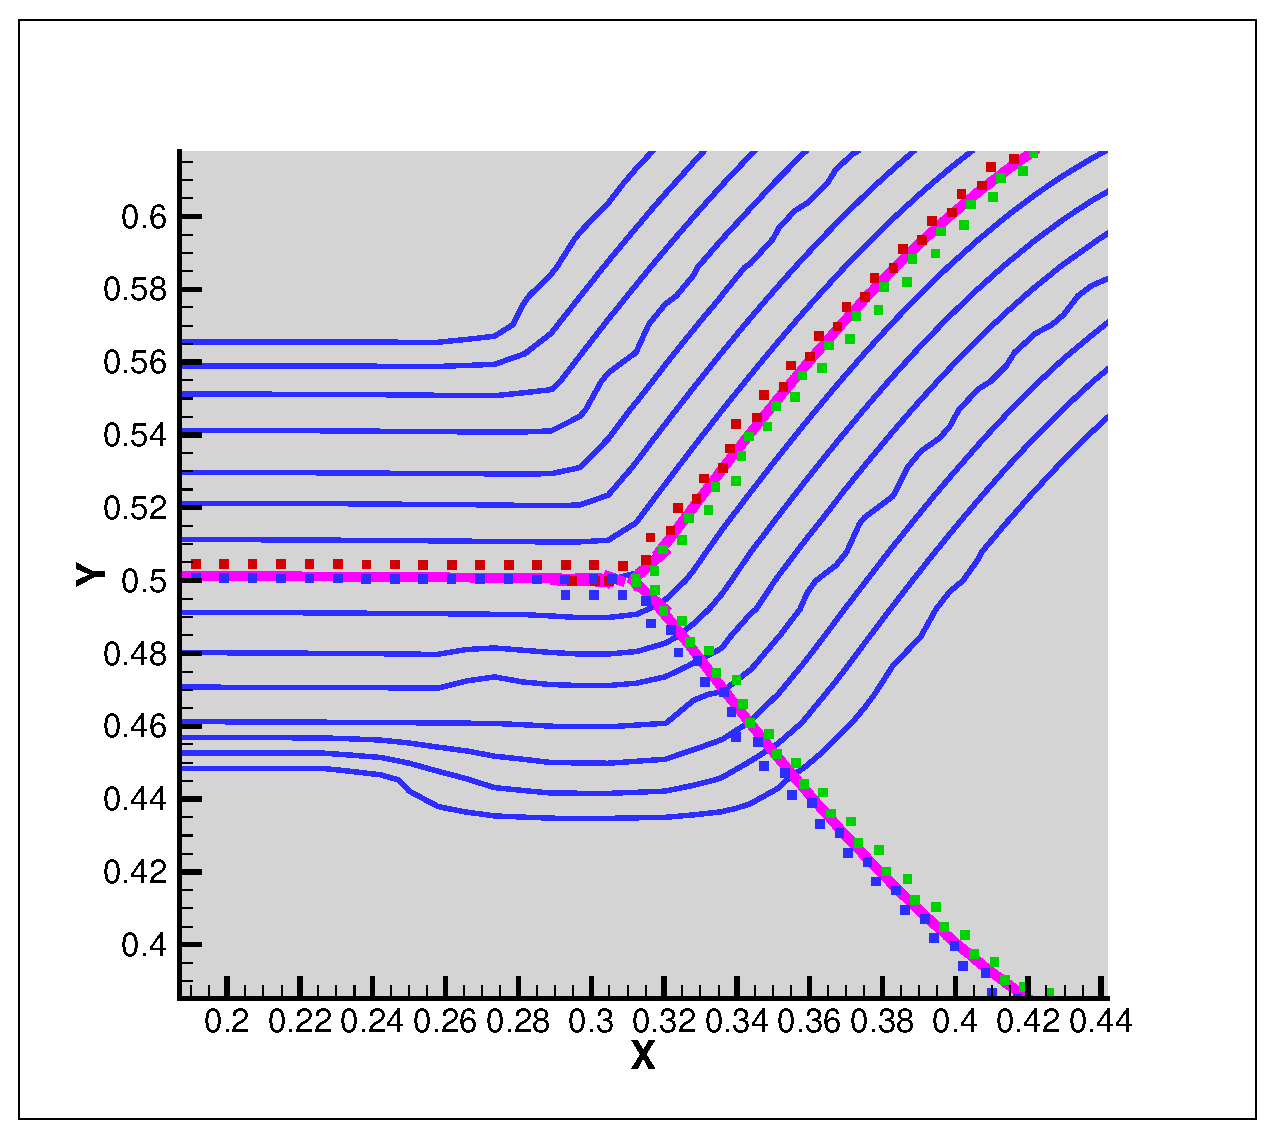
\includegraphics[width=0.45\textwidth]{zoomed_out.eps}
        \caption{Illustration of the coupled level set and 
	CMOF method corresponding to the liquid lens benchmark problem.
	LEFT: zoomed in view of (a) material 1 (signed distance function)
	level set contours (blue 
	curves), (b) normal vectors corresponding to material 1 derived 
	from the closest point map, 
	(c) CMOF reconstructed interface for all 3 materials 
	(pink curves), (d) material 1 centroids (red dots),
	(e) material 2 centroids (green dots), and
	(f) material 3 centroids (blue dots),
	RIGHT: zoomed out view.  Notes: $\Delta x=1/128$, contour
	spacing is $0.01$, the initial location of the triple point ($t=0$)
	is intentially offset from the grid lines $(0.501,0.501)$,
	tecplot level set data interpolated from the cell
	centers to the nodes.
    }
  \label{distancefunction}
\end{figure}


\section{Mathematical model}
We simulate the flow of a multiphase system consisting of $M_{fluid}$
fluid (deforming) materials and $M_{rigid}$ non-deforming materials.
The $M_{fluid}$ materials tessellate the computational domain and in the
case that a fluid material $m_{fluid}$ coincides with a rigid material,
$m_{rigid}$, the rigid materials' governing equations take precedence.
Otherwise, in regions where fluid materials and rigid materials do not
overlap, the fluid materials are
governed by the incompressible Navier-Stokes equations of immiscible
flows.   We refer the reader to Figures \ref{tank_levelset},
\ref{ice_levelset}, and \ref{liquid_lens} for illustrations which 
distinguish between deforming (tessellating) materials and non-deforming
(rigid) materials.
\begin{itemize}
\item \textbf{Material domain and interface:}
Mathematically, the domain of rigid \emph{material} $m_{rigid}$ is the 
region in which $\phi_{m_{rigid}}>0$:
\begin{equation}
  \phi_{m_{rigid}}(\mb{x},t) = \left\{
    \begin{array}{ll}
      > 0 & \mb{x} \in \tn{material}\,\: m_{rigid}, \\ 
      \leq 0 & \tn{otherwise},
  \end{array}
\right.
\end{equation}
$\bmx$ is the position vector in space and $t$ is time. 
The domain of \emph{material} $m_{fluid}$ is the 
region in which $\phi_{m_{fluid}}>0$ and 
$\phi_{m_{rigid}}<0$:
\begin{equation}
  \phi_{m_{fluid}}(\mb{x},t) = \left\{
    \begin{array}{ll}
      > 0 & \mb{x} \in \tn{material}\,\: m_{fluid}\cup m_{fluid,ghost}, \\ 
      \leq 0 & \tn{otherwise},
  \end{array}
\right.
\end{equation}

The \emph{interface} level set,
$\phi_{m1,m2}$
represents the interface between materials
$m1$ and $m2$
\begin{equation}
  \phi_{m1,m2}(\mb{x},t) = \left\{
    \begin{array}{ll}
      > 0 & \mb{x} \in \tn{material}\,\: m1, \\ 
      < 0 & \mb{x} \in \tn{material}\,\: m2, \\ 
      = 0 & \mb{x}\,\: \tn{along}\,\:(m1,m2)\,\:\tn{interface}. \\ 
    \end{array}
\right.
\end{equation}
The normal and curvature defined based on these level set functions are:
\begin{equation}
  \mb{n}_{m1,m2} = 
   \frac{\nabla \phi_{m1,m2}}{|\nabla \phi_{m1,m2}|}, \hspace{10pt}   
   \kappa_{m1,m2} = 
   \nabla \cdot \frac{\nabla \phi_{m1,m2}}{|\nabla \phi_{m1,m2}|}.
\end{equation}
\item \textbf{Conservation of mass:}
We assume that each fluid material, $m_{fluid}$, is incompressible, 
so that the velocity 
field $\bmu = (u, v, w)$ is divergence free within the bulk of each
fluid material:
\begin{equation}
  \label{eq:cnt}
  \nabla \cdot \bmu = 0.
\end{equation}
In order to account for phase change or otherwise sources and sinks of mass,
we have the following conditions on $\nabla \cdot \bmu$:
\begin{eqnarray*}
\nabla \cdot \bmu = 
  \sum_{\mbox{sources}} 
  \frac{\dot{m}_{\mbox{source}}}
       {\rho_{\mbox{source}}}\delta(\phi_{m_{\mbox{source}}}) -
  \sum_{\mbox{sinks}} 
  \frac{\dot{m}_{\mbox{sink}}}
       {\rho_{\mbox{sink}}}\delta(\phi_{m_{\mbox{sink}}}) 
\end{eqnarray*}

$H(\phi)$ is the Heaviside function which is defined as,
\begin{eqnarray*}
	H(\phi)=\left\{ \begin{array}{cc}
		1 & \phi>0  \\
  		0 & \phi\le 0 \end{array} 
	\right.
\end{eqnarray*}
$\delta(\phi)$ is the Dirac Delta function,
\begin{eqnarray*}
	\delta(\phi)=H'(\phi).
\end{eqnarray*}
%units of k: watts/(m Kelvin)=kg m/(s^3 Kelvin)
%units of L: J/kg
%1 WATT=1 Joule/s=kg m^2/s^3
%1 Joule=kg m^2/s^2
%k grad T/L units=kg m/(s^3 Kelvin)  *  (Kelvin/m)  * (kg/J)=
%kg^2/(s^3 J)=kg^2/(s kg m^2)=kg/(m^2 s)
For boiling examples,
$\dot{m}$ is the mass flux of boiling 
liquid across the liquid/vapor interface,
% e.g. liquid on left, vapor on right
% \bmn=-1
% grad T_{l}<0
% grad T_{v}>0
% \dot{m}>0
\begin{eqnarray*}
  \dot{m} = 
  \frac{k_{l}\nabla T_{l}\cdot \bmn_{l,v} - 
        k_{v}\nabla T_{v}\cdot \bmn_{l,v}}{L},
\end{eqnarray*}
where 
$k_{l}$ and $k_{v}$ are the thermal conductivities in the 
liquid and ambient vapor regions respectively, $\rho_{l}$ and
$\rho_{v}$ are the densities in the liquid and ambient vapor
regions respectively, $L$ is the latent heat of vaporization,
and $\bmn_{l,v}$ is the interface normal vector pointing from the
ambient vapor region into the liquid,
\begin{eqnarray*}
	\bmn_{l,v} = \frac{\nabla\phi_{l,v}}{|\nabla\phi_{l,v}|}.
\end{eqnarray*}


\item \textbf{Conservation of momentum:}
The conservation of momentum for each material in its domain is given by
\begin{eqnarray}
 (\bmu\rho_{m})_{t}+
  \nabla\cdot(\bmu \otimes \bmu \rho_{m}+p_{m} \EyeTen)=
  \label{eq:NS} \\
  \nabla\cdot(2\mu_{m}\DefTen)+
  \rho_{m}\bmg (1-\alpha_{m}(T_{m}-T_{0m}))
  \hspace{10pt} \tn{if} \hspace{10pt} \phi_{m}(\bmx,t)>0,
  \nonumber
\end{eqnarray}
where $p_{m}$, $T_{m}$, $\alpha_{m}$, and $\mu_{m}$ are 
pressure, temperature, coefficient of thermal expansion, and 
viscosity of material $m$ respectively, 
$\mb{g}$ is the gravitational acceleration vector, and 
$\DefTen= (\nabla\bmu+(\nabla\bmu)^{T})/2$ is the rate of deformation tensor. 
\item \textbf{Conservation of energy:} 
The conservation of energy for each material in its domain is given by
\begin{equation}
  \label{eq:heat}
  (\rho_{m}C_{p,m}T_{m})_t+
  \nabla\cdot(\bmu\rho_{m}C_{p,m}T_{m})=
  \nabla\cdot ( k_{m}\nabla T_{m})
  \hspace{10pt} \tn{if} \hspace{10pt} \phi_{m}(\bmx,t)>0,
\end{equation}
where $C_{p,m}$ and $k_{m}$ are heat capacity and thermal conductivity of 
material $m$ respectively, and $T_{m}$ is the temperature. 
\item \textbf{Interfacial jump condition:}
Here, we write out the general equations for a deforming
interface changing phase.  We define $m_{s}$ and $m_{d}$ as
the material id's associated with a ``source'' material 
(e.g. boiling liquid or freezing liquid)
and ``destination'' material (e.g. vapor from boiling or ice from freezing) 
respectively.
The location of the interface separating a material $m_{s}$ region from a
material $m_{d}$ region is governed by the level set equation,
\begin{eqnarray}
\phi_{m_{s},m_{d},t} + 
\bmu_{m_{s}}\cdot\nabla\phi_{m_{s},m_{d},t} =
-\frac{\dot{m}}{\rho_{s}}|\nabla\phi_{m_{s},m_{d},t}|
\end{eqnarray}
\begin{eqnarray}
\phi_{m_{d},m_{s},t} + 
\bmu_{m_{s}}\cdot\nabla\phi_{m_{d},m_{s},t} =
\frac{\dot{m}}{\rho_{s}}|\nabla\phi_{m_{d},m_{s},t}|
\end{eqnarray}
An equivalent expression for the level set governing equations is:
\begin{eqnarray}
\phi_{m_{s},m_{d},t} + 
\bmu_{m_{d}}\cdot\nabla\phi_{m_{s},m_{d},t} =
-\frac{\dot{m}}{\rho_{d}}|\nabla\phi_{m_{s},m_{d},t}|
\end{eqnarray}
\begin{eqnarray}
\phi_{m_{d},m_{s},t} + 
\bmu_{m_{d}}\cdot\nabla\phi_{m_{d},m_{s},t} =
\frac{\dot{m}}{\rho_{d}}|\nabla\phi_{m_{d},m_{s},t}|
\end{eqnarray}
The interface jump conditions,
between two materials $m_{s}$ and $m_{d}$,
for the velocity, pressure, 
and temperature, respectively, are,
\begin{eqnarray*}
 \bmu_{m_{s}}\cdot \bmn_{m_{s},m_{d}}-
 \bmu_{m_{d}}\cdot \bmn_{m_{s},m_{d}} = 
\dot{m}(\frac{1}{\rho_{m_{d}}}-
	\frac{1}{\rho_{m_{s}}}),
\end{eqnarray*}
\begin{eqnarray*}
	(p_{m_{s}}\EyeTen-
	 p_{m_{d}}\EyeTen).\bmn_{m_{s},m_{d}}=
	-\sigma_{m_{s},m_{d}}\kappa_{m_{s},m_{d}}\bmn_{m_{s},m_{d}} + \\
	(2\mu_{m_{s}}\DefTen_{m_{s}}-
	 2\mu_{m_{d}}\DefTen_{m_{d}}).\bmn_{m_{s},m_{d}},
\end{eqnarray*}
\begin{eqnarray}
	T_{m_{s}}=
	T_{m_{d}}.
	\label{temperature_jump}
\end{eqnarray}
$\kappa_{m_{s},m_{d}}$ is the interface curvature
and is defined as,
\begin{eqnarray*}
	\kappa_{m_{s},m_{d}}=\nabla\cdot
	\frac{\nabla\phi_{m1,m2}}
             {|\nabla\phi_{m1,m2}|}.
\end{eqnarray*}

At a triple point junction a three-phase equilibrium known as the 
Neumann's triangle\cite{de2013capillarity} determines the 
angles (see Figure \ref{fig:triple_point}.a):
\begin{equation}
  \label{eq:triple_point_eqlib}
  \frac{\sin(\theta_{1})}{\sigma_{23}}=
  \frac{\sin(\theta_{2})}{\sigma_{13}}=
  \frac{\sin(\theta_{3})}{\sigma_{12}}.
\end{equation}

\end{itemize}

\begin{figure}[htbp]
  \centering
    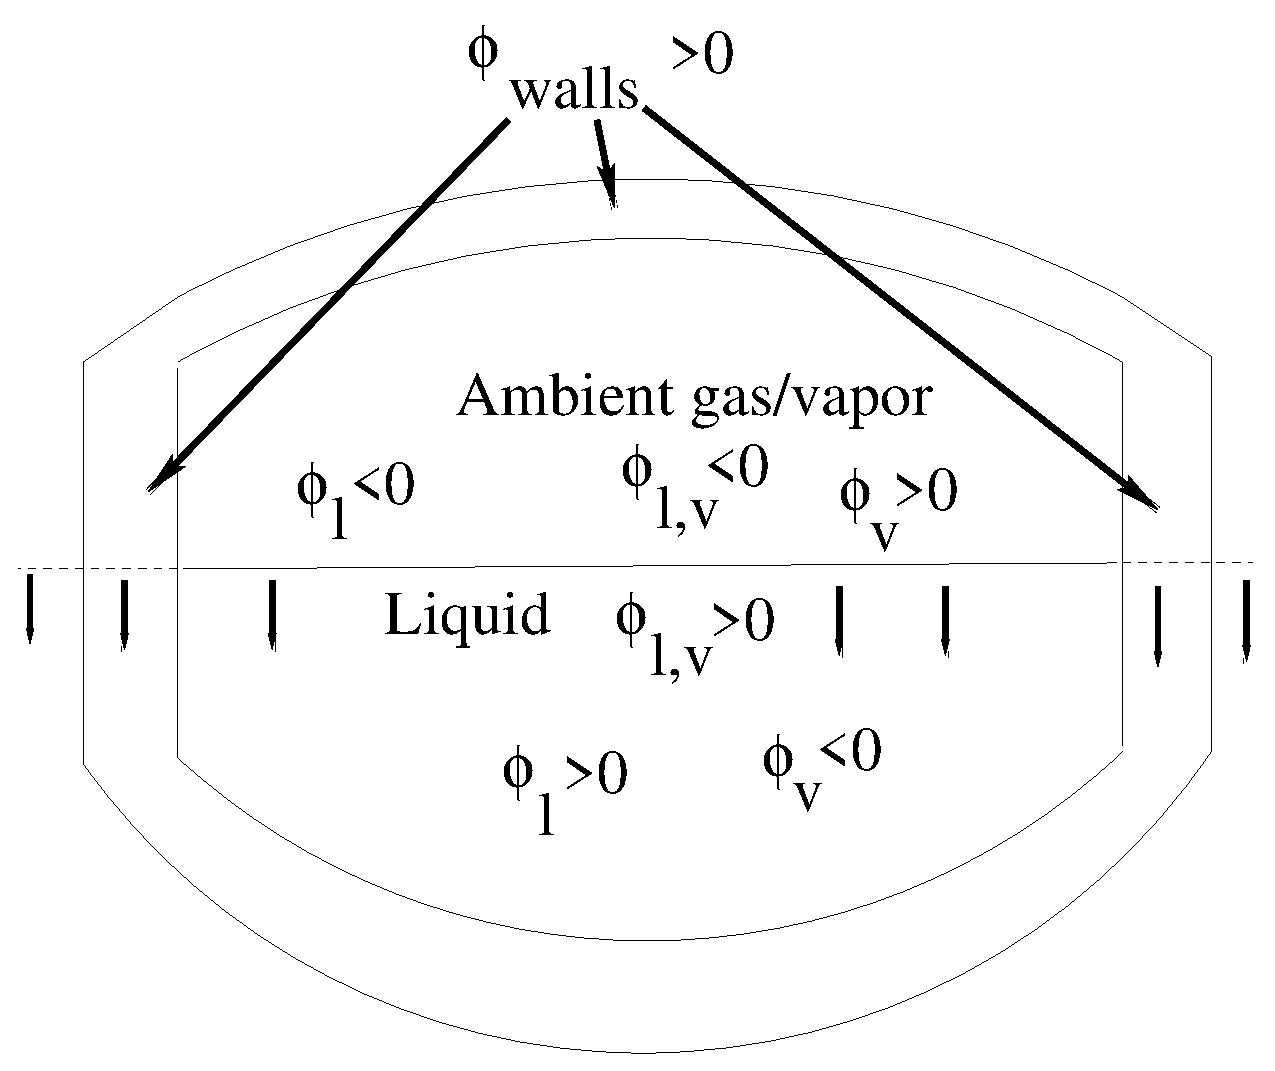
\includegraphics[width=0.7\textwidth]{tank_levelset.eps}
        \caption{Level set functions for the simulation of evaporation
        in a Cryogenic Fuel tank.  
        The liquid and vapor deforming
        materials tessellate the 
        computational domain.
        The tank walls are rigid.
        $\phi_{\mbox{walls}}>0$ in the tank walls,
        $\phi_{l,v}<0$ and $\phi_{v}>0$ 
        in the ambient vapor region, and
        $\phi_{l,v}>0$ and $\phi_{l}>0$
        in the liquid region.  The liquid/vapor interface
        is extended into the ``tank walls region.''
        Following the surface tension model described in
        \cite{li2015multiphase}, page 471, ``Stencil
        contains rigid boundary,'' we calculate the curvature
        at the liquid/vapor/solid triple point by approximating
        $\kappa=\nabla\cdot\bmn$ in which $\bmn$ is assigned 
        a strategic ``ghost normal'' in the solid region consistent
        with the contact angle condition. 
        The interfacial
        curvature away from the liquid/vapor/solid 
        triple point is computed using
        the Volume of fluid height function technique
        \cite{sussman2003second}.
    }
  \label{tank_levelset}
\end{figure}

\begin{figure}[htbp]
  \centering
    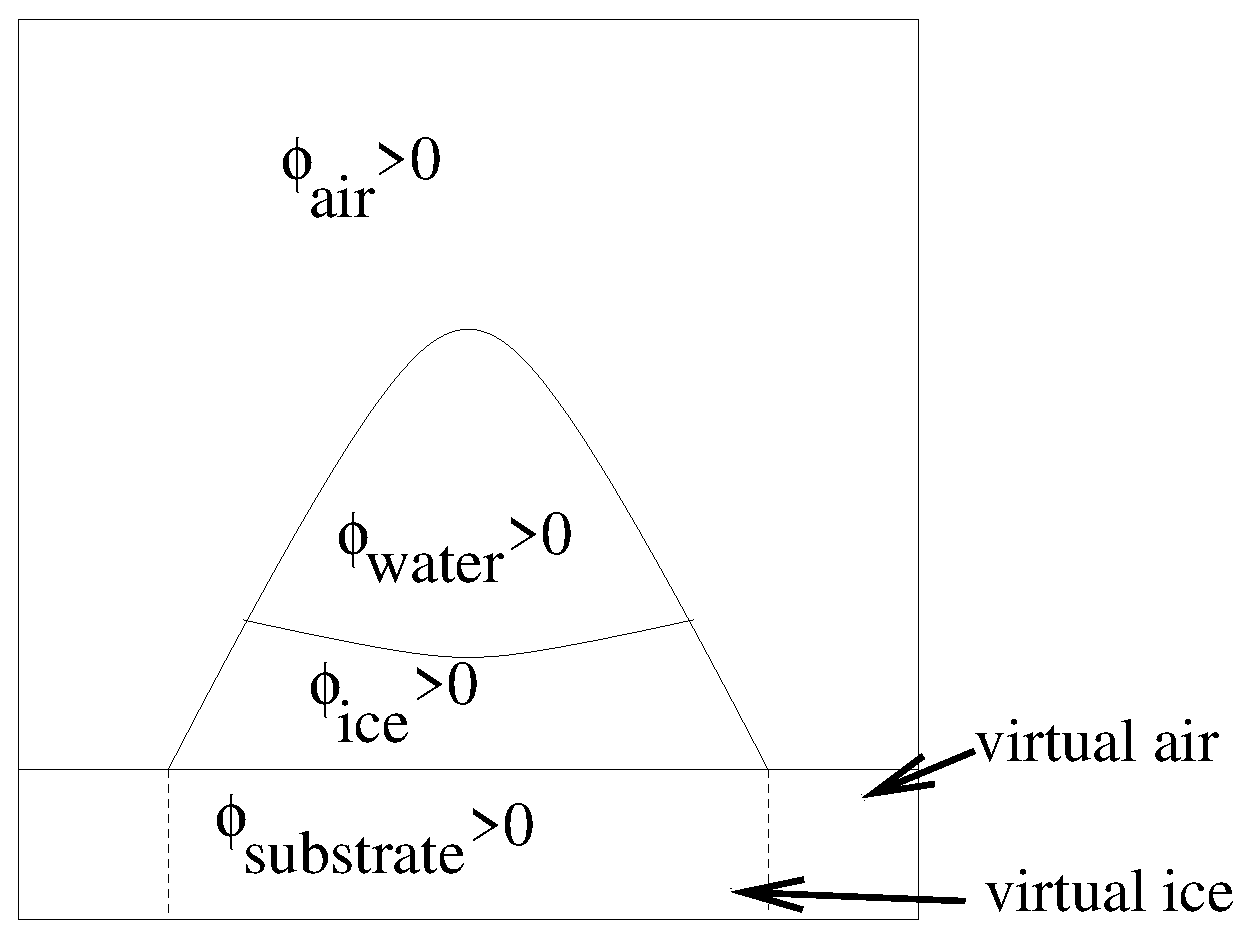
\includegraphics[width=0.7\textwidth]{ice_levelset.eps}
        \caption{Level set functions for the simulation of 
	the freezing of a water drop on top of a cold substrate.
	The temperature in the substrate, $T_{w}$, is prescribed.
        The ice, water, and air deforming materials tessellate
        the computational domain.
        $\phi_{\mbox{substrate}}>0$ in the cold substrate,
        $\phi_{\mbox{ice}}>0$ in the ice and 
        $\phi_{\mbox{water}}>0$ in the water.  The
        ice/air interface is extended into the substrate.
        Note: the ice is a deforming material solely due to 
        phase change at the ice/water interface.
        Following the freezing model presented in \cite{lyu2021hybrid}, the
        ice and water materials are considered as the same
        material when calculating the surface tension force 
        at the water/ice/air triple point.
        In other words, the interfacial
        curvature both at and away from triple points is computed using
        the Volume of fluid height function technique
        \cite{sussman2003second}.
    }
  \label{ice_levelset}
\end{figure}


\begin{figure}[htbp]
  \centering
    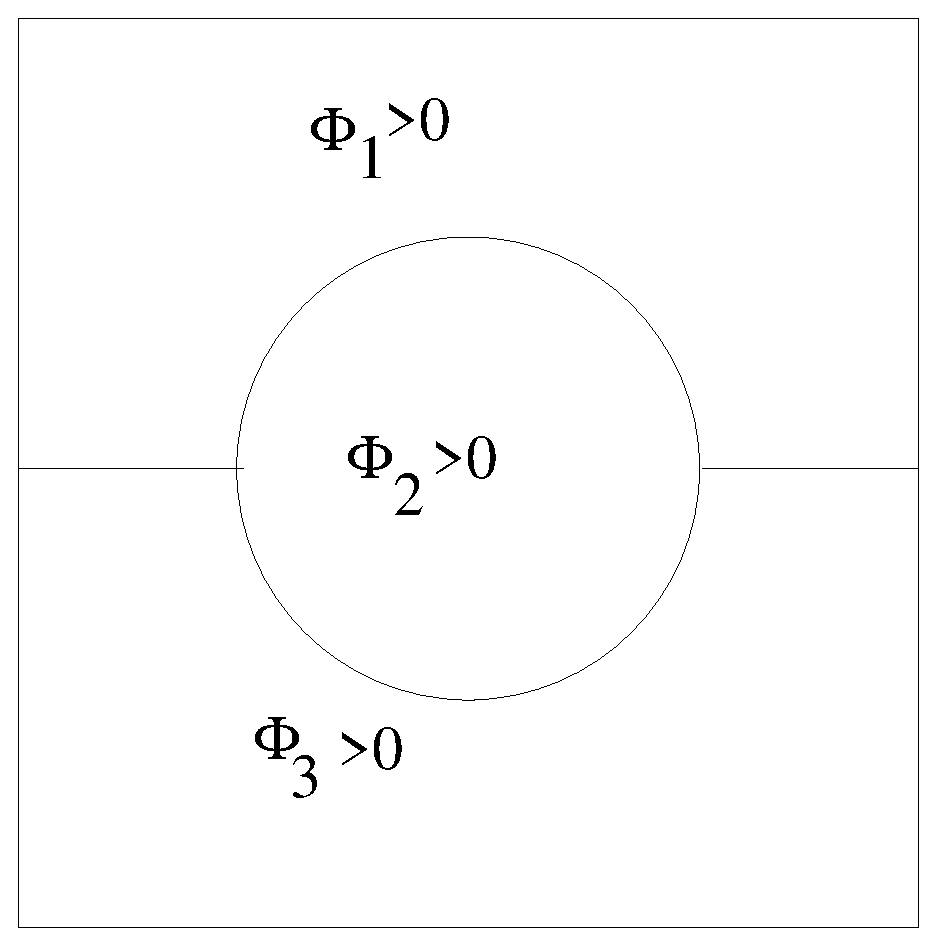
\includegraphics[width=0.7\textwidth]{liquid_lens.eps}
        \caption{Level set functions for the simulation of 
        the stretching of a ``liquid lens'' due to surface 
        tension.  The lens material $\phi_{2}$ and surrounding
        materials, $\phi_{1}$ and $\phi_{3}$, are all deforming
        fluids so that these three materials tessellate the
        computational domain.
        Following the surface tension model described in
        \cite{li2015multiphase}, page 472, ``Stencil
        contains third fluid,''         
        the surface tension force at the triple point(s) are 
        calculated as
        $\sum_{m=1}^{M} \gamma_{m}\kappa_{m}\nabla H(\phi_{m})$
        in which $\kappa_{m}$ is approximated by way of finite
        differences of the level set function(s) $\phi$. 
        The interfacial
        curvature away from triple points is computed using
        the Volume of fluid height function technique
        \cite{sussman2003second}.
    }
  \label{liquid_lens}
\end{figure}


\section{Numerical methods and algorithms}

We describe our numerical method for the 
2D uniform rectangular Cartesian grid
case.  
In the problem domain, a computational cell, $\Omega_{i,j}$, is defined as,
\begin{eqnarray}
  \label{eq:cell_def}
  \Omega_{i,j} = 
   \left\{ \bmx: x \in \left[x_i-\frac{\Delta x}{2}, x_i+\frac{\Delta x}{2}\right],\right.\\
   \left. y \in \left[ y_i-\frac{\Delta y}{2}, y_i+\frac{\Delta y}{2}\right] \right\}
\end{eqnarray}
where $\bmx_{i,j} = \left\{x_i,y_j\right\}$ is the 
center of the cell $\Omega_{i,j}$. The domain of 
material $m$ in a cell at time $t^n$ is denoted by $\Omega_{m,i,j}^n$, 
and the zeroth and first order moments of the $m$th material 
distribution, corresponding to the volume fraction and 
centroid position, are defined as,
\begin{equation}
  \label{eq:moments_def}
  F_{m,i,j}^n = \frac{\int_{\Omega_{m,i,j}^n} ~\mathrm{d} \Omega}{V_{i,j}}, \hspace{0.5cm}\bmx_{m,i,j}^{c,n} = \frac{\int_{\Omega_{m,i,j}^n} \bmx ~\mathrm{d} \Omega}{V_{i,j,m}^n},
\end{equation}
where the computational cell volume is $V_{i,j} = \int_{\Omega_{i,j}} ~\mathrm{d} \Omega$, and volume of the portion for material $m$ in a computational cell is $V_{i,j,m}^n= \int_{\Omega_{m,i,j}^n} ~\mathrm{d} \Omega$. The discretization for a typical point around the triple point is shown in Figure \ref{fig:triple_point}.
\begin{figure}[htbp]
  \centering
  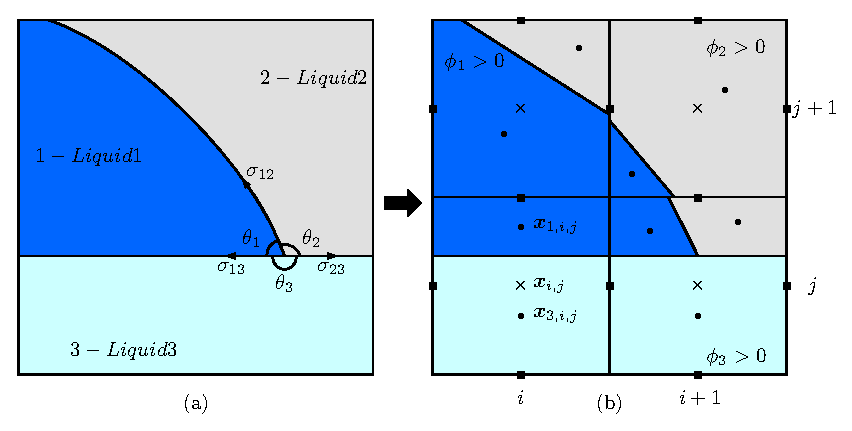
\includegraphics[width=0.8\textwidth]{triple_point_drop_impact.eps}
%%  \scalebox{0.75}
%%  { %%Created by jPicEdt 1.4.1_03: mixed JPIC-XML/LaTeX format
%%Fri May 06 19:00:30 EDT 2016
%%Begin JPIC-XML
%<?xml version="1.0" standalone="yes"?>
%<jpic x-min="0" x-max="134.87" y-min="0" y-max="65" auto-bounding="true">
%<multicurve fill-style= "solid"
%	 points= "(0,5);(0,10);(0,15);(0,25);(10,25);(55,25);
%	(60,25);(60,20);(60,10);(60,5);(55,5);(5,5)"
%	 fill-color= "#ccffff"
%	 stroke-style= "none"
%	 />
%<multicurve fill-style= "solid"
%	 points= "(5,65);(0,65);(5,65);(0,65);(0,60);(0,30);
%	(0,25);(5,25);(10,25);(15,25);(25,25);(30,25);
%	(45,25);(40,40);(20,60)"
%	 fill-color= "#0066ff"
%	 stroke-style= "none"
%	 />
%<multicurve fill-style= "solid"
%	 points= "(60,65);(50,65);(15,65);(5,65);(20,60);(40,40);
%	(45,25);(55,25);(55,25);(60,25);(60,30);(60,60)"
%	 fill-color= "#e1e1e1"
%	 stroke-style= "none"
%	 />
%<parallelogram p3= "(60,65)"
%	 p2= "(60,5)"
%	 p1= "(0,5)"
%	 fill-style= "none"
%	 />
%<multicurve fill-style= "none"
%	 points= "(45,25);(40,40);(20,60);(5,65)"
%	 />
%<multicurve fill-style= "none"
%	 points= "(60,25);(50,25);(10,25);(0,25)"
%	 />
%<text text-vert-align= "center-v"
%	 fill-style= "none"
%	 anchor-point= "(11.89,41.89)"
%	 text-frame= "noframe"
%	 text-hor-align= "center-h"
%	 >
%$1-Liquid 1$
%</text>
%<text text-vert-align= "center-v"
%	 fill-style= "none"
%	 anchor-point= "(10,55)"
%	 text-frame= "noframe"
%	 text-hor-align= "center-h"
%	 >
%
%</text>
%<text text-vert-align= "center-v"
%	 fill-style= "none"
%	 anchor-point= "(50,55)"
%	 text-frame= "noframe"
%	 text-hor-align= "center-h"
%	 >
%$2-Liquid 2$
%</text>
%<text text-vert-align= "center-v"
%	 fill-style= "none"
%	 anchor-point= "(17.81,9.04)"
%	 text-frame= "noframe"
%	 text-hor-align= "center-h"
%	 >
%$3-Liquid 3$
%</text>
%<multicurve arrow-head-width-minimum= "0.5"
%	 right-arrow= "head"
%	 fill-style= "none"
%	 arrow-head-length-scale= "1.5"
%	 points= "(45,25);(42,25);(41,25);(35,25)"
%	 arrow-head-inset-scale= "0"
%	 />
%<multicurve arrow-head-width-minimum= "0.5"
%	 right-arrow= "head"
%	 fill-style= "none"
%	 arrow-head-length-scale= "1.5"
%	 points= "(45,25);(42.96,30.43);(41.12,33.68);(37.83,38.12)"
%	 arrow-head-inset-scale= "0"
%	 />
%<multicurve arrow-head-width-minimum= "0.5"
%	 right-arrow= "head"
%	 fill-style= "none"
%	 arrow-head-length-scale= "1.5"
%	 points= "(45,25);(49,25);(51,25);(54,25)"
%	 arrow-head-inset-scale= "0"
%	 />
%<text text-vert-align= "center-v"
%	 fill-style= "none"
%	 anchor-point= "(53,23)"
%	 text-frame= "noframe"
%	 text-hor-align= "center-h"
%	 >
%$\sigma_{23}$
%</text>
%<text text-vert-align= "center-v"
%	 fill-style= "none"
%	 anchor-point= "(36,23)"
%	 text-frame= "noframe"
%	 text-hor-align= "center-h"
%	 >
%$\sigma_{13}$
%</text>
%<text text-vert-align= "center-v"
%	 fill-style= "none"
%	 anchor-point= "(41,39)"
%	 text-frame= "noframe"
%	 text-hor-align= "center-h"
%	 >
%$\sigma_{12}$
%</text>
%<multicurve fill-style= "none"
%	 points= "(42,25);(42.04,26.38);(42.73,27.27);(43.95,27.63)"
%	 />
%<multicurve fill-style= "none"
%	 points= "(44.26,27.04);(46.09,27.11);(47.17,26.41);(47.6,25.07)"
%	 />
%<text text-vert-align= "center-v"
%	 fill-style= "none"
%	 anchor-point= "(41,28)"
%	 text-frame= "noframe"
%	 text-hor-align= "right"
%	 >
%$\theta_1$
%</text>
%<text text-vert-align= "center-v"
%	 fill-style= "none"
%	 anchor-point= "(48,28)"
%	 text-frame= "noframe"
%	 text-hor-align= "left"
%	 >
%$\theta_2$
%</text>
%<multicurve fill-style= "solid"
%	 points= "(75,65);(75,65);(130,65);(130,65);(130,65);(130,25);
%	(130,25);(130,25);(115,25);(115,25);(115.1,25);(110,35);
%	(110,35);(110,35);(111,35);(111,35);(111,35);(100,48);
%	(100,48);(100,48);(100,49);(100,49);(100,49);(75,65)"
%	 fill-color= "#e1e1e1"
%	 />
%<multicurve fill-style= "solid"
%	 points= "(70,5);(70,5);(70,25);(70,25);(70,25);(120,25);
%	(120,25);(120,25);(120,25);(120,25);(120,25);(125,25);
%	(125,25);(125,25);(130,25);(130,25);(130,25);(130,20);
%	(130,20);(130,20);(130,10);(130,10);(130,10);(130,5);
%	(130,5);(130,5);(70,5)"
%	 fill-color= "#ccffff"
%	 />
%<multicurve fill-style= "solid"
%	 points= "(70,65);(70,65);(75,65);(75,65);(75,65);(100,49);
%	(100,49);(100,49);(100,48);(100,48);(100,48);(111,35);
%	(111,35);(111,35);(110,35);(110,35);(110,35);(115,25);
%	(115,25);(115,25);(70,25);(70,25);(70,25);(70,65)"
%	 fill-color= "#0066ff"
%	 />
%<parallelogram p3= "(130,65)"
%	 p2= "(130,5)"
%	 p1= "(70,5)"
%	 fill-style= "none"
%	 />
%<text text-vert-align= "center-v"
%	 fill-style= "none"
%	 anchor-point= "(77.14,57.84)"
%	 text-frame= "noframe"
%	 text-hor-align= "center-h"
%	 >
%$\phi_1&gt;0$
%</text>
%<text text-vert-align= "center-v"
%	 fill-style= "none"
%	 anchor-point= "(80,55)"
%	 text-frame= "noframe"
%	 text-hor-align= "center-h"
%	 >
%
%</text>
%<text text-vert-align= "center-v"
%	 fill-style= "none"
%	 anchor-point= "(121.42,60.34)"
%	 text-frame= "noframe"
%	 text-hor-align= "center-h"
%	 >
%$\phi_2&gt;0$
%</text>
%<text text-vert-align= "center-v"
%	 fill-style= "none"
%	 anchor-point= "(121.49,7.91)"
%	 text-frame= "noframe"
%	 text-hor-align= "center-h"
%	 >
%$\phi_3&gt;0$
%</text>
%<multicurve fill-style= "none"
%	 points= "(70,35);(70,35);(130,35);(130,35)"
%	 />
%<multicurve fill-style= "none"
%	 points= "(100,5);(100,5);(100,65);(100,65)"
%	 />
%<multicurve polydots-scale-h= "1"
%	 polydots-scale-v= "1"
%	 polydots-style= "polydots-disk"
%	 polydots-angle= "0"
%	 fill-style= "solid"
%	 polydots-size-linewidth-scale= "0.5"
%	 polydots-size-minimum= "0.7"
%	 points= "(85,30);(85,30);(85,15);(85,15);(85,15);(115,15);
%	(115,15);(115,15);(121.75,30.88);(121.75,30.88);(121.75,30.88);(119.47,53.16);
%	(119.47,53.16);(119.47,53.16);(94.74,60.35);(94.74,60.35);(94.74,60.35);(82.11,45.7);
%	(82.11,45.7);(82.11,45.7);(103.68,38.95);(103.68,38.95);(103.68,38.95);(106.75,29.39);
%	(106.75,29.39)"
%	 polydots-superimpose= "false"
%	 />
%<multicurve polydots-scale-h= "1"
%	 polydots-scale-v= "1"
%	 polydots-style= "polydots-square-filled"
%	 polydots-angle= "0"
%	 fill-style= "solid"
%	 polydots-size-linewidth-scale= "1.5"
%	 polydots-size-minimum= "0.7"
%	 points= "(85,65);(85,65);(85,35);(85,35);(85,35);(85,5);
%	(85,5);(85,5);(115,5);(115,5);(115,5);(115,35);
%	(115,35);(115,35);(115,65);(115,65);(115,65);(85,65)"
%	 stroke-style= "none"
%	 polydots-superimpose= "false"
%	 />
%<multicurve polydots-scale-h= "1"
%	 polydots-scale-v= "1"
%	 polydots-style= "polydots-square-filled"
%	 polydots-angle= "0"
%	 fill-style= "solid"
%	 polydots-size-linewidth-scale= "1.5"
%	 polydots-size-minimum= "0.7"
%	 points= "(70,50);(70,50);(100,50);(100,50);(100,50);(130,50);
%	(130,50);(130,50);(130,20);(130,20);(130,20);(100,20);
%	(100,20);(100,20);(70,20);(70,20);(70,20);(70,50)"
%	 polydots-superimpose= "false"
%	 />
%<multicurve fill-style= "solid"
%	 points= "(68,34);(68,34);(66,36);(66,36);(66,36);(66,35);
%	(66,35);(66,35);(62,35);(62,35);(62,35);(62,33);
%	(62,33);(62,33);(66,33);(66,33);(66,33);(66,32);
%	(66,32);(66,32);(68,34)"
%	 />
%<text text-vert-align= "center-v"
%	 fill-style= "none"
%	 anchor-point= "(30,0)"
%	 text-frame= "noframe"
%	 text-hor-align= "center-h"
%	 >
%(a)
%</text>
%<text text-vert-align= "center-v"
%	 fill-style= "none"
%	 anchor-point= "(100,0)"
%	 text-frame= "noframe"
%	 text-hor-align= "center-h"
%	 >
%(b)
%</text>
%<multicurve polydots-scale-h= "1"
%	 polydots-scale-v= "1"
%	 polydots-style= "polydots-plus"
%	 polydots-angle= "45"
%	 fill-style= "none"
%	 polydots-size-linewidth-scale= "3.5"
%	 polydots-size-minimum= "0.7"
%	 points= "(85,50);(85,50);(115,50);(115,50);(115,50);(115,20);
%	(115,20);(115,20);(85,20);(85,20)"
%	 polydots-superimpose= "false"
%	 />
%<text text-vert-align= "center-v"
%	 fill-style= "none"
%	 anchor-point= "(87,20)"
%	 text-frame= "noframe"
%	 text-hor-align= "left"
%	 >
%$\bmx_{i,j}$
%</text>
%<text text-vert-align= "center-v"
%	 fill-style= "none"
%	 anchor-point= "(87,15)"
%	 text-frame= "noframe"
%	 text-hor-align= "left"
%	 >
%$\bmx_{3,i,j}$
%</text>
%<text text-vert-align= "center-v"
%	 fill-style= "none"
%	 anchor-point= "(87,30)"
%	 text-frame= "noframe"
%	 text-hor-align= "left"
%	 >
%$\bmx_{1,i,j}$
%</text>
%<text text-vert-align= "center-v"
%	 fill-style= "none"
%	 anchor-point= "(85,1.18)"
%	 text-frame= "noframe"
%	 text-hor-align= "center-h"
%	 >
%$i$
%</text>
%<text text-vert-align= "center-v"
%	 fill-style= "none"
%	 anchor-point= "(115.4,1.05)"
%	 text-frame= "noframe"
%	 text-hor-align= "center-h"
%	 >
%$i+1$
%</text>
%<text text-vert-align= "center-v"
%	 fill-style= "none"
%	 anchor-point= "(134.47,20)"
%	 text-frame= "noframe"
%	 text-hor-align= "center-h"
%	 >
%$j$
%</text>
%<text text-vert-align= "center-v"
%	 fill-style= "none"
%	 anchor-point= "(134.87,49.87)"
%	 text-frame= "noframe"
%	 text-hor-align= "center-h"
%	 >
%$j+1$
%</text>
%<multicurve fill-style= "none"
%	 points= "(47,25);(47,22);(43,22);(43,25)"
%	 />
%<text text-vert-align= "center-v"
%	 fill-style= "none"
%	 anchor-point= "(45.03,20.46)"
%	 text-frame= "noframe"
%	 text-hor-align= "center-h"
%	 >
%$\theta_3$
%</text>
%</jpic>
%%End JPIC-XML
%PSTricks content-type (pstricks.sty package needed)
%Add \usepackage{pstricks} in the preamble of your LaTeX file
%You can rescale the whole picture (to 80% for instance) by using the command \def\JPicScale{0.8}
\ifx\JPicScale\undefined\def\JPicScale{1}\fi
\psset{unit=\JPicScale mm}
\psset{linewidth=0.3,dotsep=1,hatchwidth=0.3,hatchsep=1.5,shadowsize=1,dimen=middle}
\psset{dotsize=0.7 2.5,dotscale=1 1,fillcolor=black}
\psset{arrowsize=1 2,arrowlength=1,arrowinset=0.25,tbarsize=0.7 5,bracketlength=0.15,rbracketlength=0.15}
\begin{pspicture}(0,0)(134.87,65)
\newrgbcolor{userFillColour}{0.8 1 1}
\pscustom[linestyle=none,fillcolor=userFillColour,fillstyle=solid]{\psbezier(0,5)(0,10)(0,15)(0,25)
\psbezier(10,25)(55,25)(60,25)
\psbezier(60,20)(60,10)(60,5)
\psbezier(55,5)(5,5)(0,5)
\closepath}
\newrgbcolor{userFillColour}{0 0.4 1}
\pscustom[linestyle=none,fillcolor=userFillColour,fillstyle=solid]{\psbezier(5,65)(0,65)(5,65)(0,65)
\psbezier(0,60)(0,30)(0,25)
\psbezier(5,25)(10,25)(15,25)
\psbezier(25,25)(30,25)(45,25)
\psbezier(40,40)(20,60)(5,65)
\closepath}
\newrgbcolor{userFillColour}{0.88 0.88 0.88}
\pscustom[linestyle=none,fillcolor=userFillColour,fillstyle=solid]{\psbezier(60,65)(50,65)(15,65)(5,65)
\psbezier(20,60)(40,40)(45,25)
\psbezier(55,25)(55,25)(60,25)
\psbezier(60,30)(60,60)(60,65)
\closepath}
\pspolygon[](0,5)(60,5)(60,65)(0,65)
\psbezier(45,25)(40,40)(20,60)(5,65)
\psbezier(60,25)(50,25)(10,25)(0,25)
\rput(11.89,41.89){$1-Liquid 1$}
\rput(10,55){}
\rput(50,55){$2-Liquid 2$}
\rput(17.81,9.04){$3-Liquid 3$}
\psbezier[arrowsize=0.5 2,arrowlength=1.5,arrowinset=0]{->}(45,25)(42,25)(41,25)(35,25)
\psbezier[arrowsize=0.5 2,arrowlength=1.5,arrowinset=0]{->}(45,25)(42.96,30.43)(41.12,33.68)(37.83,38.12)
\psbezier[arrowsize=0.5 2,arrowlength=1.5,arrowinset=0]{->}(45,25)(49,25)(51,25)(54,25)
\rput(53,23){$\sigma_{23}$}
\rput(36,23){$\sigma_{13}$}
\rput(41,39){$\sigma_{12}$}
\psbezier(42,25)(42.04,26.38)(42.73,27.27)(43.95,27.63)
\psbezier(44.26,27.04)(46.09,27.11)(47.17,26.41)(47.6,25.07)
\rput[r](41,28){$\theta_1$}
\rput[l](48,28){$\theta_2$}
\newrgbcolor{userFillColour}{0.88 0.88 0.88}
\pscustom[fillcolor=userFillColour,fillstyle=solid]{\psline(75,65)(130,65)
\psline(130,65)(130,25)
\psline(130,25)(115,25)
\psbezier(115.1,25)(110,35)(110,35)
\psline(110,35)(111,35)
\psline(111,35)(100,48)
\psline(100,48)(100,49)
\psline(100,49)(75,65)
\closepath}
\newrgbcolor{userFillColour}{0.8 1 1}
\pscustom[fillcolor=userFillColour,fillstyle=solid]{\psline(70,5)(70,25)
\psline(70,25)(120,25)
\psbezier(120,25)(120,25)(120,25)
\psline(120,25)(125,25)
\psline(125,25)(130,25)
\psline(130,25)(130,20)
\psline(130,20)(130,10)
\psline(130,10)(130,5)
\psline(130,5)(70,5)
\closepath}
\newrgbcolor{userFillColour}{0 0.4 1}
\pspolygon[fillcolor=userFillColour,fillstyle=solid](70,65)
(75,65)
(100,49)
(100,48)
(111,35)
(110,35)
(115,25)
(70,25)(70,65)
\pspolygon[](70,5)(130,5)(130,65)(70,65)
\rput(77.14,57.84){$\phi_1>0$}
\rput(80,55){}
\rput(121.42,60.34){$\phi_2>0$}
\rput(121.49,7.91){$\phi_3>0$}
\psline(70,35)(130,35)
\psline(100,5)(100,65)
\psdots[fillstyle=solid,dotsize=0.7 0.5](85,30)
(85,15)(115,15)(121.75,30.88)(119.47,53.16)(94.74,60.35)(82.11,45.7)(103.68,38.95)(106.75,29.39)
\psdots[linestyle=none,fillstyle=solid,dotsize=0.7 1.5,dotstyle=square*](85,65)
(85,35)(85,5)(115,5)(115,35)(115,65)
\psdots[fillstyle=solid,dotsize=0.7 1.5,dotstyle=square*](70,50)
(100,50)(130,50)(130,20)(100,20)(70,20)
\pspolygon[fillstyle=solid](68,34)
(66,36)
(66,35)
(62,35)
(62,33)
(66,33)
(66,32)(68,34)
\rput(30,0){(a)}
\rput(100,0){(b)}
\psdots[dotsize=0.7 3.5,dotstyle=+,dotangle=45](85,50)
(115,50)(115,20)(85,20)
\rput[l](87,20){$\bmx_{i,j}$}
\rput[l](87,15){$\bmx_{3,i,j}$}
\rput[l](87,30){$\bmx_{1,i,j}$}
\rput(85,1.18){$i$}
\rput(115.4,1.05){$i+1$}
\rput(134.47,20){$j$}
\rput(134.87,49.87){$j+1$}
\psbezier(47,25)(47,22)(43,22)(43,25)
\rput(45.03,20.46){$\theta_3$}
\end{pspicture}
 }
  \caption{(a) Physical domain: a part of the problem domain containing a triple point. Surface tension forces are at equilibrium determining the contact angles. (b) Discretized domain: crosses show cell centers, circles represent cell centroids and horizontal and vertical rectangles depict the MAC grid points in each cell.}
  \label{fig:triple_point}
\end{figure}


\subsection{method overview: Staggered grid Projection Method}

Referring to Figure \ref{fig:ch2_nodeslocation} and also 
\cite{pei2019hierarchical,VAHAB2021}, 
we discretize the velocity on the marker-and-cell (MAC) grid and we
discretize pressure, temperature, level set function(s), volume fraction(s),
and centroid(s) at the center of grid cells.

An outline of our operator split method is as 
follows 
(\cite{VAHAB2021}):
\begin{itemize}
\item \textbf{Calculate the time step $\Delta t=t^{n+1}-t^{n}$:}
  \begin{eqnarray*}
  \Delta t_{1}=\mbox{min}_{d=1,\ldots,\mbox{D}}
    \frac{\mbox{min}\Delta x_{d}}{2 D \mbox{max}|u_{d}^{n}|} 
    \hspace{15pt} \mbox{D}=2\mbox{ or }3
  \end{eqnarray*}
  \begin{eqnarray*}
  \Delta t_{2}=
    \mbox{min}_{d=1,\ldots,\mbox{D}}
    \frac{\mbox{min}\Delta x_{d}}{D\mbox{max}
    |u_{d}^{\mbox{phase change},n-1}|} 
  \end{eqnarray*}
  \begin{eqnarray}
  \Delta t_{3}=
  \mbox{min}_{d=1,\ldots,D}
  \mbox{min}_{m1,m2=1,\ldots,M}
    \Delta x_{d}^{3/2}
    \sqrt{\frac{\rho_{m1}+\rho_{m2}}
          {2\pi\sigma_{m1,m2}}} 
    \label{stiffconstraint}
  \end{eqnarray}
  \begin{eqnarray*}
  \Delta t=\mbox{CFL}\mbox{min}(
    \Delta t_{1},
    \Delta t_{2},
    \Delta t_{3}) \hspace{15pt} \mbox{CFL}=1/2
  \end{eqnarray*}
  
\item \textbf{Cell Integrated Semi-Lagrangian (CISL) MAC velocity advection
  (see\cite{pei2019hierarchical}):}
  \begin{eqnarray}
  (\rho \bmu)_{t}+\nabla\cdot(\rho\bmu\bmu)=0, \label{advection}
  \end{eqnarray}
\item \textbf{CISL temperature advection
  (liquid and gas materials, see \cite{VAHAB2021}):}
  \begin{eqnarray}
  (\rho_{m} C_{p,m} T_{m})_{t}+
  \nabla\cdot(\rho_{m} C_{p,m} \bmu T_{m})=0, \hspace{10pt}
  m=1,\ldots,M \label{adv2}
  \end{eqnarray}
\item \textbf{CISL level set advection:}
  \begin{eqnarray*}
  \phi_{m,t}+\bmu\cdot\nabla\phi_{m}=0, \hspace{10pt} 
  m=1,\ldots,M 
  \end{eqnarray*}
\item \textbf{CISL advection of the Volume fractions and Centroids
 (see \cite{jemison2013coupled,jemison2014compressible,li2015multiphase,pei2019hierarchical,VAHAB2021}):}
  \begin{eqnarray}
  F_{m,t}+\nabla\cdot(\bmu F_{m})=0, \hspace{10pt}
  m=1,\ldots,M  \label{eq:transport}
  \end{eqnarray}
\item \textbf{Coupling the level set functions to the volume fractions and Centroids:}
  The (continuous) 
  moment-of-fluid reconstructed
  (see Section \ref{MOF_vs_CMOF_sec}) 
  slope initial guess uses the level set functions,
  and the level set functions are in turn replaced by the exact 
  signed distance (see Section \ref{MMRECON}) 
  to the continuous moment-of-fluid reconstructed
  interface.
\item \textbf{Phase change velocity from material $m_{s}$ (source) to material $m_{d}$ (destination)
  (see \cite{VAHAB2021} and \cite{liu2022novel}):}
  \begin{eqnarray}
  \bmu^{\mbox{phase change}}=-\frac{\dot{m}}{\rho_{m_{d}}}\bmn_{m_{d}},
  \label{uphasechange}
  \end{eqnarray}
\item \textbf{Phase change: Level Set Advection:}
  \begin{eqnarray*}
  \phi_{m,t}+\bmu^{\mbox{phase change}}\cdot\nabla\phi_{m}=0,
  \hspace{10pt} m=m_{s} \mbox{ or } m_{d}.
  \end{eqnarray*}
\item \textbf{Phase change: unsplit CISL advection of the Volume fractions and Centroids
  (see \cite{VAHAB2021,liu2022novel}):}
  \begin{eqnarray*}
  F_{m,t}+\nabla\cdot(\bmu^{\mbox{phase change}}F_{m})=0,
  \hspace{10pt} m=m_{s} \mbox{ or } m_{d}.
  \end{eqnarray*}
\item \textbf{Phase change: Coupling the level set functions to the volume fractions and Centroids:} 
  The (continuous) 
  moment-of-fluid reconstructed
  (see Section \ref{MOF_vs_CMOF_sec}) 
  slope initial guess uses the level set functions,
  and the level set functions are in turn replaced by the exact 
  signed distance (see Section \ref{MMRECON}) 
  to the continuous moment-of-fluid reconstructed
  interface.
\item \textbf{Phase change: Mass source redistribution:} 
  Redistribute $\dot{m}$ to the
  source material, $m_{s}$, side (e.g. liquid if boiling or 
  freezing) \cite{VAHAB2021}.
\item \textbf{Thermal diffusion
  (see \cite{VAHAB2021} for algorithmic details):}
  \begin{eqnarray}
  \frac{(\rho C_{p,m})^{\mbox{mix},n+1}}{\Delta t^{\mbox{swept}}}
  (T^{n+1}_{m}-T^{\mbox{advection}}_{m})=
   \nabla\cdot (k_{m} \nabla T^{n+1}_{m})
  \label{diffusion1}
  \end{eqnarray}
\item \textbf{Viscosity
  (see \cite{pei2019hierarchical} for algorithmic details):}
  \begin{eqnarray}
	  \frac{\rho^{\mbox{mix},n+1}}{\Delta t}
	  (\bmu^{\ast}-\bmu^{\mbox{advection}})=
	  \nabla\cdot(2\mu\DefTen^{\ast})-
	  \rho^{n+1}(\alpha^{n+1}(T^{n+1}-T_{0}))\bmg
	  \label{diffusion3}
  \end{eqnarray}
\item \textbf{Pressure Gradient (liquid and vapor regions)
  (see 
  \cite{jemison2014compressible,li2015multiphase,pei2019hierarchical,VAHAB2021} 
  for algorithmic details):}
  \begin{eqnarray}
  \frac{\bmu^{n+1}-\bmu^{\ast}}{\Delta t}=
    -\frac{\nabla p^{n+1}}{\rho^{\mbox{MAC,mix},n+1}}+\bmg-
    \frac{\sum_{m=1}^{M} \gamma_{m}\kappa_{m}\nabla H(\phi_{m})}
         {\rho^{\mbox{MAC,mix},n+1}}
	  \label{pressuregrad}
  \end{eqnarray}
  \begin{eqnarray*}
  \nabla \cdot \bmu^{n+1} = 
   \sum_{\mbox{sources}} 
   \frac{\dot{m}_{\mbox{source}}}
        {\rho_{\mbox{source}}}\delta(\phi_{m_{\mbox{source}}}) -
   \sum_{\mbox{sinks}} 
   \frac{\dot{m}_{\mbox{sink}}}
        {\rho_{\mbox{sink}}}\delta(\phi_{m_{\mbox{sink}}}) 
  \end{eqnarray*}
  For the case in which two materials, $m1$ and $m2$,
  are present in a given $3\times 3$
  stencil,
   %% remember: \kappa_{m1}=-\kappa_{m2}, H(\phi_{m1})=1-H(\phi_{m2})
  \begin{eqnarray*}
  \gamma_{m1}=\gamma_{m2}=\frac{\sigma_{m1,m2}}{2} 
  \end{eqnarray*}
  and for the case when three materials, $m1$, $m2$, $m3$, are
  present in a given $3\times 3$ stencil,
  \begin{eqnarray*}
  \gamma_{m1}=\frac{\sigma_{m1,m2}+\sigma_{m1,m3}-\sigma_{m2,m3}}{2} 
  \end{eqnarray*}
  \begin{eqnarray*}
  \gamma_{m2}=\frac{\sigma_{m1,m2}+\sigma_{m2,m3}-\sigma_{m1,m3}}{2} 
  \end{eqnarray*}
  \begin{eqnarray*}
  \gamma_{m3}=\frac{\sigma_{m1,m3}+\sigma_{m2,m3}-\sigma_{m1,m2}}{2} 
  \end{eqnarray*}

\end{itemize}


\begin{figure}[htbp] 
  \centering
    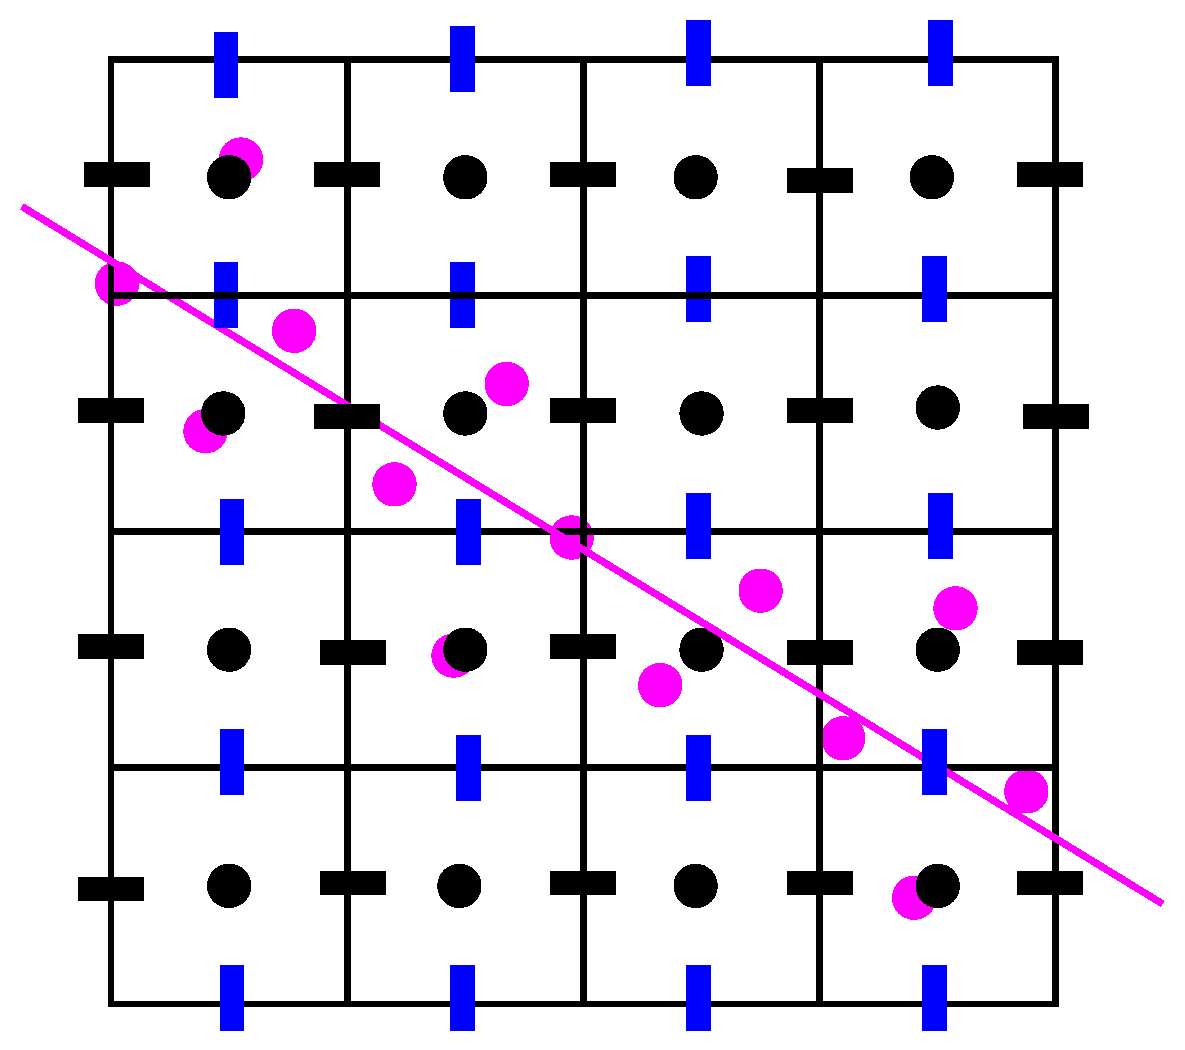
\includegraphics[width=0.7\textwidth]{stag_uniform.eps}
  \caption{
   An illustration of the locations on our 
   (staggered) computational grid
   in which fluid variables are approximated.
   Pressure, level set function(s), volume fraction(s), and 
   centroids are discretized at the cell centers (filled in black circles).
   The horizontal velocity, $u$, 
   is discretized at the midpoint of cell faces
   with constant $x$ value (filled in black rectangles), and the 
   vertical velocity, $v$,
   is discretized at the midpoint of cell faces with constant $y$ value
   (filled in blue rectangles).
   The material centroids are denoted by the filled in magenta circles.
   }
  \label{fig:ch2_nodeslocation} 
\end{figure}

Remarks:
\begin{enumerate}
\item For step 2 ``phase change'' above, we use MOF interface
 reconstruction.   Our rationale is that (1) the phase change
 velocity $\bmu^{\mbox{phase change}}$ is not  
 determined from the interface curvature, so that there is no
 instability risk due to MOF advection here, and (2) MOF is
 more accurate than CMOF in this scenario.
\item We use the multigrid preconditioned conjugate gradient 
 method \cite{tatebe1993multigrid}
 to solve the large sparse matrix system that
 results from discretizing (\ref{diffusion1}).  The discretization
 of the Dirichlet interface temperature condition due to 
 phase change uses the second order method described in 
 \cite{gibou2002second}.
\item We also use the multigrid preconditioned conjugate gradient (MGPCG)
 method \cite{tatebe1993multigrid}
 to solve the large sparse matrix system that
 results from discretizing (\ref{pressuregrad}).  In order
 to simulate flows in sealed tanks or flows induced by the 
 sealing of a valve \cite{arienti2014embedded} we have developed a general 
 method for enforcing the solvability condition in each 
 ``enclosed'' region.  We identify each ``enclosed'' region
 using a shading method developed by \cite{sussman2009stable}.
\item In order to preserve mass for phase change problems, we
  must prescribe a stringent tolerance for the pressure equation
  (\ref{pressuregrad}).  In some cases, due to round off error, the
  MGPCG method might stall.  In order to overcome the effect of 
  round-off error, we keep track of a history of the pressure
  admitting the least residual, and, when the solver has stalled,
  we restart the MGPCG process using the
  previous best guess pressure and
  increasing the number of multigrid relaxation steps by 1.
\end{enumerate}

\subsection{MOF and Continuous MOF interface reconstruction methods
  \label{MOF_vs_CMOF_sec} }
The original MOF reconstruction method is local to the cell and 
uses the reference volume fraction, $F_\tn{ref} \equiv F_{m,i,j}^n$, 
and reference centroid, $\bmx_\tn{ref}^c \equiv \bmx_{m,i,j}^n$ to 
find the linear (planer) interface reconstruction that has the volume
fraction equal to $F_\tn{ref}$, and has the least amount of error 
for centroid position. We find the actual volume fraction 
$F_\tn{act}(\bmn,b)$ and centroid $\bmx_\tn{act}^c(\bmn,b)$ 
for a reconstructed line(plane) with the normal $\bmn$ and 
intercept $b$ which minimizes
\begin{equation}
  E_\tn{MOF} = \lVert \bmx_\tn{ref}^c - \bmx_\tn{act}^c(\bmn,b) \rVert_2
\end{equation}
while $F_\tn{act}(\bmn,b) = F_\tn{ref}$ (see Figure
\ref{fig:mof_reconstruction}).
\begin{figure}[htbp]
  \centering
  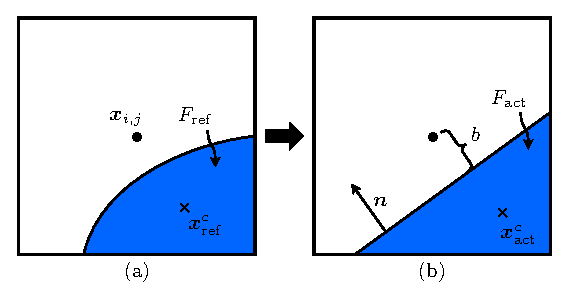
\includegraphics[width=0.8\textwidth]{mof_reconstruction.eps}
%%  \scalebox{1.0}
%%  { %%Created by jPicEdt 1.4.1_03: mixed JPIC-XML/LaTeX format
%%Sat Mar 05 01:28:45 EST 2016
%%Begin JPIC-XML
%<?xml version="1.0" standalone="yes"?>
%<jpic x-min="0" x-max="90" y-min="-3" y-max="40" auto-bounding="true">
%<multicurve fill-style= "solid"
%	 fill-color= "#0066ff"
%	 points= "(57,0);(57,0);(90,0);(90,0);(90,0);(90,24);
%	(90,24);(90,24);(57,0)"
%	 />
%<multicurve fill-style= "solid"
%	 fill-color= "#0066ff"
%	 points= "(11,0);(18,0);(32,0);(40,0);(40,7);(40,13);
%	(40,20);(30,19);(14,13)"
%	 />
%<parallelogram stroke-width= "0.4"
%	 p3= "(40,0)"
%	 fill-style= "none"
%	 p2= "(40,40)"
%	 p1= "(0,40)"
%	 />
%<parallelogram stroke-width= "0.4"
%	 p3= "(90,0)"
%	 fill-style= "none"
%	 p2= "(90,40)"
%	 p1= "(50,40)"
%	 />
%<multicurve fill-style= "none"
%	 points= "(11,0);(14,13);(30,19);(40,20)"
%	 />
%<multicurve fill-style= "none"
%	 points= "(57,0);(57,0);(90,24);(90,24)"
%	 />
%<multicurve polydots-angle= "0"
%	 polydots-style= "polydots-disk"
%	 fill-style= "none"
%	 polydots-size-linewidth-scale= "2.5"
%	 polydots-size-minimum= "0.7"
%	 polydots-superimpose= "false"
%	 points= "(20,20);(20,20);(70,20);(70,20)"
%	 polydots-scale-v= "1"
%	 polydots-scale-h= "1"
%	 />
%<multicurve polydots-angle= "45"
%	 polydots-style= "polydots-plus"
%	 fill-style= "none"
%	 polydots-size-linewidth-scale= "3.5"
%	 polydots-size-minimum= "0.8"
%	 polydots-superimpose= "false"
%	 points= "(28,8);(28,8);(82,7);(82,7)"
%	 polydots-scale-v= "1"
%	 polydots-scale-h= "1"
%	 />
%<multicurve right-arrow= "head"
%	 fill-style= "none"
%	 points= "(62,4);(62,4);(56.35,11.89);(56.35,11.89)"
%	 />
%<multicurve fill-style= "none"
%	 points= "(71.5,20.61);(72.49,21.29);(72.94,20.63);(73.05,20.46);(73.16,20.3);(74.07,18.97);
%	(74.18,18.81);(74.29,18.64);(74.74,17.98);(75.73,18.66);(74.74,17.98);(75.19,17.32);
%	(75.3,17.16);(75.42,16.99);(76.32,15.67);(76.43,15.5);(76.54,15.34);(76.99,14.68);
%	(76,14)"
%	 />
%<text text-vert-align= "top"
%	 fill-style= "none"
%	 anchor-point= "(28.65,6.62)"
%	 text-frame= "noframe"
%	 text-hor-align= "left"
%	 >
%$\bmx_\textnormal{ref}^c$
%</text>
%<text text-vert-align= "bottom"
%	 fill-style= "none"
%	 anchor-point= "(27,22)"
%	 text-frame= "noframe"
%	 text-hor-align= "left"
%	 >
%$F_\textnormal{ref}$
%</text>
%<text text-vert-align= "top"
%	 fill-style= "none"
%	 anchor-point= "(81.51,5)"
%	 text-frame= "noframe"
%	 text-hor-align= "left"
%	 >
%$\bmx_\textnormal{act}^c$
%</text>
%<text text-vert-align= "bottom"
%	 fill-style= "none"
%	 anchor-point= "(80,25)"
%	 text-frame= "noframe"
%	 text-hor-align= "left"
%	 >
%$F_\textnormal{act}$
%</text>
%<multicurve right-arrow= "head"
%	 fill-style= "none"
%	 points= "(32,21);(32.03,18.04);(33.24,18.99);(33.31,14.8)"
%	 />
%<text text-vert-align= "bottom"
%	 fill-style= "none"
%	 anchor-point= "(60,8.11)"
%	 text-frame= "noframe"
%	 text-hor-align= "left"
%	 >
%$\bmn$
%</text>
%<text text-vert-align= "center-v"
%	 fill-style= "none"
%	 anchor-point= "(76.76,19.59)"
%	 text-frame= "noframe"
%	 text-hor-align= "center-h"
%	 >
%
%</text>
%<text text-vert-align= "bottom"
%	 fill-style= "none"
%	 anchor-point= "(76.54,19.14)"
%	 text-frame= "noframe"
%	 text-hor-align= "left"
%	 >
%$b$
%</text>
%<text text-vert-align= "top"
%	 fill-style= "none"
%	 anchor-point= "(15.35,24.32)"
%	 text-frame= "noframe"
%	 text-hor-align= "left"
%	 >
%$\bmx_{i,j}$
%</text>
%<multicurve fill-style= "solid"
%	 points= "(48,20);(48,20);(46,22);(46,22);(46,22);(46,21);
%	(46,21);(46,21);(42,21);(42,21);(42,21);(42,19);
%	(42,19);(42,19);(46,19);(46,19);(46,19);(46,18);
%	(46,18);(46,18);(48,20)"
%	 />
%<multicurve right-arrow= "head"
%	 fill-style= "none"
%	 points= "(85,24);(85.03,21.04);(86.24,21.99);(86.31,17.8)"
%	 />
%<text text-vert-align= "center-v"
%	 fill-style= "none"
%	 anchor-point= "(20,-3)"
%	 text-frame= "noframe"
%	 text-hor-align= "center-h"
%	 >
%(a)
%</text>
%<text text-vert-align= "center-v"
%	 fill-style= "none"
%	 anchor-point= "(70,-3)"
%	 text-frame= "noframe"
%	 text-hor-align= "center-h"
%	 >
%(b)
%</text>
%</jpic>
%%End JPIC-XML
%PSTricks content-type (pstricks.sty package needed)
%Add \usepackage{pstricks} in the preamble of your LaTeX file
%You can rescale the whole picture (to 80% for instance) by using the command \def\JPicScale{0.8}
\ifx\JPicScale\undefined\def\JPicScale{1}\fi
\psset{unit=\JPicScale mm}
\psset{linewidth=0.3,dotsep=1,hatchwidth=0.3,hatchsep=1.5,shadowsize=1,dimen=middle}
\psset{dotsize=0.7 2.5,dotscale=1 1,fillcolor=black}
\psset{arrowsize=1 2,arrowlength=1,arrowinset=0.25,tbarsize=0.7 5,bracketlength=0.15,rbracketlength=0.15}
\begin{pspicture}(0,0)(90,40)
\newrgbcolor{userFillColour}{0 0.4 1}
\pspolygon[fillcolor=userFillColour,fillstyle=solid](57,0)
(90,0)
(90,24)(57,0)
\newrgbcolor{userFillColour}{0 0.4 1}
\pscustom[fillcolor=userFillColour,fillstyle=solid]{\psbezier(11,0)(18,0)(32,0)(40,0)
\psbezier(40,7)(40,13)(40,20)
\psbezier(30,19)(14,13)(11,0)
\closepath}
\pspolygon[linewidth=0.4](0,40)(40,40)(40,0)(0,0)
\pspolygon[linewidth=0.4](50,40)(90,40)(90,0)(50,0)
\psbezier(11,0)(14,13)(30,19)(40,20)
\psline(57,0)(90,24)
\psdots[](20,20)
(70,20)
\psdots[dotsize=0.8 3.5,dotstyle=+,dotangle=45](28,8)
(82,7)
\psline{->}(62,4)(56.35,11.89)
\pscustom[]{\psbezier(71.5,20.61)(72.49,21.29)(72.94,20.63)(73.05,20.46)
\psbezier(73.16,20.3)(74.07,18.97)(74.18,18.81)
\psbezier(74.29,18.64)(74.74,17.98)(75.73,18.66)
\psbezier(74.74,17.98)(75.19,17.32)(75.3,17.16)
\psbezier(75.42,16.99)(76.32,15.67)(76.43,15.5)
\psbezier(76.54,15.34)(76.99,14.68)(76,14)
}
\rput[tl](28.65,6.62){$\bmx_\textnormal{ref}^c$}
\rput[bl](27,22){$F_\textnormal{ref}$}
\rput[tl](81.51,5){$\bmx_\textnormal{act}^c$}
\rput[bl](80,25){$F_\textnormal{act}$}
\psbezier{->}(32,21)(32.03,18.04)(33.24,18.99)(33.31,14.8)
\rput[bl](60,8.11){$\bmn$}
\rput(76.76,19.59){}
\rput[bl](76.54,19.14){$b$}
\rput[tl](15.35,24.32){$\bmx_{i,j}$}
\pspolygon[fillstyle=solid](48,20)
(46,22)
(46,21)
(42,21)
(42,19)
(46,19)
(46,18)(48,20)
\psbezier{->}(85,24)(85.03,21.04)(86.24,21.99)(86.31,17.8)
\rput(20,-3){(a)}
\rput(70,-3){(b)}
\end{pspicture}
 }
  \caption{(a) Material domain at cell $\{i,j\}$ for one of the 
phases, and corresponding reference volume fraction and centroid. 
(b) Piecewise linear reconstruction of the interface using MOF 
method. The line segment can be represented as 
$\Omega_{i,j} \cap \{ \bmx | \bmn \cdot (\bmx - \bmx_{i,j}) + b = 0 \}$}
  \label{fig:mof_reconstruction}
\end{figure}
Starting from a whole cell and repeating this process 
while only considering the uncaptured regions from previous 
steps, we can reconstruct the material interface for 
each phase in a multimaterial cell (see \cite{li2015multiphase} 
for algorithm details). This tessellating procedure 
generates a volume preserving reconstruction 
at triple-points (see Figure \ref{fig:mof_tes_nontes}).
\begin{figure}[htbp]
  \centering
  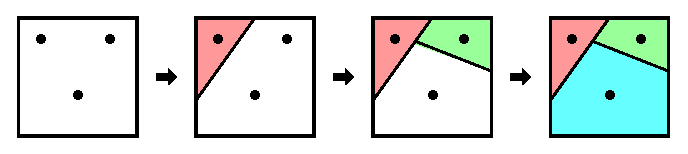
\includegraphics[width=0.8\textwidth]{mof_tes.eps}
%%  \scalebox{0.75}
%%  { %%Created by jPicEdt 1.4.1_03: mixed JPIC-XML/LaTeX format
%%Tue Jul 12 12:16:29 EDT 2016
%%Begin JPIC-XML
%<?xml version="1.0" standalone="yes"?>
%<jpic x-min="0" x-max="110" y-min="0" y-max="20" auto-bounding="true">
%<parallelogram p3= "(20,20)"
%	 p2= "(20,0)"
%	 p1= "(0,0)"
%	 fill-style= "none"
%	 stroke-width= "0.4"
%	 />
%<multicurve polydots-superimpose= "false"
%	 polydots-angle= "0"
%	 polydots-size-linewidth-scale= "2.5"
%	 polydots-style= "polydots-disk"
%	 fill-style= "none"
%	 polydots-scale-v= "1"
%	 points= "(3.65,16.49);(3.65,16.49);(10,7);(10,7);(10,7);(15.3,16.55);
%	(15.3,16.55)"
%	 polydots-scale-h= "1"
%	 polydots-size-minimum= "0.7"
%	 />
%<multicurve pstcustom= "opacity=0.5"
%	 stroke-style= "none"
%	 fill-style= "solid"
%	 fill-color= "#ff9999"
%	 points= "(30,6);(30,6);(40,20);(40,20);(40,20);(36,20);
%	(36,20);(36,20);(30,20);(30,20);(30,20);(30,15);
%	(30,15);(30,15);(30,6)"
%	 />
%<parallelogram p3= "(50,20)"
%	 p2= "(50,0)"
%	 p1= "(30,0)"
%	 fill-style= "none"
%	 stroke-width= "0.4"
%	 />
%<multicurve polydots-superimpose= "false"
%	 polydots-angle= "0"
%	 polydots-size-linewidth-scale= "2.5"
%	 polydots-style= "polydots-disk"
%	 fill-style= "none"
%	 polydots-scale-v= "1"
%	 points= "(33.65,16.49);(33.65,16.49);(40,7);(40,7);(40,7);(45.3,16.55);
%	(45.3,16.55)"
%	 polydots-scale-h= "1"
%	 polydots-size-minimum= "0.7"
%	 />
%<multicurve fill-style= "none"
%	 points= "(40,20);(40,20);(30,6);(30,6)"
%	 />
%<multicurve pstcustom= "opacity=0.5"
%	 stroke-style= "none"
%	 fill-style= "solid"
%	 fill-color= "#99ff99"
%	 points= "(66,16);(66,16);(80,11);(80,11);(80,11);(80,20);
%	(80,20);(80,20);(74,20);(74,20);(74,20);(70,20);
%	(70,20);(70,20);(66,16)"
%	 />
%<multicurve pstcustom= "opacity=0.5"
%	 stroke-style= "none"
%	 fill-style= "solid"
%	 fill-color= "#ff9999"
%	 points= "(60,6);(60,6);(70,20);(70,20);(70,20);(66,20);
%	(66,20);(66,20);(60,20);(60,20);(60,20);(60,15);
%	(60,15);(60,15);(60,6)"
%	 />
%<parallelogram p3= "(80,20)"
%	 p2= "(80,0)"
%	 p1= "(60,0)"
%	 fill-style= "none"
%	 stroke-width= "0.4"
%	 />
%<multicurve polydots-superimpose= "false"
%	 polydots-angle= "0"
%	 polydots-size-linewidth-scale= "2.5"
%	 polydots-style= "polydots-disk"
%	 fill-style= "none"
%	 polydots-scale-v= "1"
%	 points= "(63.65,16.49);(63.65,16.49);(70,7);(70,7);(70,7);(75.3,16.55);
%	(75.3,16.55)"
%	 polydots-scale-h= "1"
%	 polydots-size-minimum= "0.7"
%	 />
%<multicurve fill-style= "none"
%	 points= "(70,20);(70,20);(60,6);(60,6)"
%	 />
%<multicurve fill-style= "none"
%	 points= "(67.23,16.01);(67.23,16.01);(80,11);(80,11)"
%	 />
%<multicurve pstcustom= "opacity=0.5"
%	 stroke-style= "none"
%	 fill-style= "solid"
%	 fill-color= "#99ff99"
%	 points= "(96,16);(96,16);(110,11);(110,11);(110,11);(110,20);
%	(110,20);(110,20);(104,20);(104,20);(104,20);(100,20);
%	(100,20);(100,20);(96,16)"
%	 />
%<multicurve pstcustom= "opacity=0.5"
%	 stroke-style= "none"
%	 fill-style= "solid"
%	 fill-color= "#ff9999"
%	 points= "(90,6);(90,6);(100,20);(100,20);(100,20);(96,20);
%	(96,20);(96,20);(90,20);(90,20);(90,20);(90,15);
%	(90,15);(90,15);(90,6)"
%	 />
%<multicurve pstcustom= "opacity=0.5"
%	 stroke-style= "none"
%	 fill-style= "solid"
%	 fill-color= "#66ffff"
%	 points= "(90,0);(90,0);(110,0);(110,0);(110,0);(110,11);
%	(110,11);(110,11);(97,16);(97,16);(97,16);(90,6);
%	(90,6);(90,6);(90,0)"
%	 />
%<parallelogram p3= "(110,20)"
%	 p2= "(110,0)"
%	 p1= "(90,0)"
%	 fill-style= "none"
%	 stroke-width= "0.4"
%	 />
%<multicurve polydots-superimpose= "false"
%	 polydots-angle= "0"
%	 polydots-size-linewidth-scale= "2.5"
%	 polydots-style= "polydots-disk"
%	 fill-style= "none"
%	 polydots-scale-v= "1"
%	 points= "(93.65,16.49);(93.65,16.49);(100,7);(100,7);(100,7);(105.3,16.55);
%	(105.3,16.55)"
%	 polydots-scale-h= "1"
%	 polydots-size-minimum= "0.7"
%	 />
%<multicurve fill-style= "none"
%	 points= "(100,20);(100,20);(90,6);(90,6)"
%	 />
%<multicurve fill-style= "none"
%	 points= "(97.23,16.01);(97.23,16.01);(110,11);(110,11)"
%	 />
%<multicurve fill-style= "solid"
%	 points= "(26.5,10);(26.5,10);(25.5,11);(25.5,11);(25.5,11);(25.5,10.5);
%	(25.5,10.5);(25.5,10.5);(23.5,10.5);(23.5,10.5);(23.5,10.5);(23.5,9.5);
%	(23.5,9.5);(23.5,9.5);(25.5,9.5);(25.5,9.5);(25.5,9.5);(25.5,9);
%	(25.5,9);(25.5,9);(26.5,10)"
%	 />
%<multicurve fill-style= "solid"
%	 points= "(86.5,10);(86.5,10);(85.5,11);(85.5,11);(85.5,11);(85.5,10.5);
%	(85.5,10.5);(85.5,10.5);(83.5,10.5);(83.5,10.5);(83.5,10.5);(83.5,9.5);
%	(83.5,9.5);(83.5,9.5);(85.5,9.5);(85.5,9.5);(85.5,9.5);(85.5,9);
%	(85.5,9);(85.5,9);(86.5,10)"
%	 />
%<multicurve fill-style= "solid"
%	 points= "(56.5,10);(56.5,10);(55.5,11);(55.5,11);(55.5,11);(55.5,10.5);
%	(55.5,10.5);(55.5,10.5);(53.5,10.5);(53.5,10.5);(53.5,10.5);(53.5,9.5);
%	(53.5,9.5);(53.5,9.5);(55.5,9.5);(55.5,9.5);(55.5,9.5);(55.5,9);
%	(55.5,9);(55.5,9);(56.5,10)"
%	 />
%</jpic>
%%End JPIC-XML
%PSTricks content-type (pstricks.sty package needed)
%Add \usepackage{pstricks} in the preamble of your LaTeX file
%You can rescale the whole picture (to 80% for instance) by using the command \def\JPicScale{0.8}
\ifx\JPicScale\undefined\def\JPicScale{1}\fi
\psset{unit=\JPicScale mm}
\psset{linewidth=0.3,dotsep=1,hatchwidth=0.3,hatchsep=1.5,shadowsize=1,dimen=middle}
\psset{dotsize=0.7 2.5,dotscale=1 1,fillcolor=black}
\psset{arrowsize=1 2,arrowlength=1,arrowinset=0.25,tbarsize=0.7 5,bracketlength=0.15,rbracketlength=0.15}
\begin{pspicture}(0,0)(110,20)
\pspolygon[linewidth=0.4](0,0)(20,0)(20,20)(0,20)
\psdots[](3.65,16.49)
(10,7)(15.3,16.55)
\newrgbcolor{userFillColour}{1 0.6 0.6}
\pspolygon[linestyle=none,fillcolor=userFillColour,fillstyle=solid,opacity=0.5](30,6)
(40,20)
(36,20)
(30,20)
(30,15)(30,6)
\pspolygon[linewidth=0.4](30,0)(50,0)(50,20)(30,20)
\psdots[](33.65,16.49)
(40,7)(45.3,16.55)
\psline(40,20)(30,6)
\newrgbcolor{userFillColour}{0.6 1 0.6}
\pspolygon[linestyle=none,fillcolor=userFillColour,fillstyle=solid,opacity=0.5](66,16)
(80,11)
(80,20)
(74,20)
(70,20)(66,16)
\newrgbcolor{userFillColour}{1 0.6 0.6}
\pspolygon[linestyle=none,fillcolor=userFillColour,fillstyle=solid,opacity=0.5](60,6)
(70,20)
(66,20)
(60,20)
(60,15)(60,6)
\pspolygon[linewidth=0.4](60,0)(80,0)(80,20)(60,20)
\psdots[](63.65,16.49)
(70,7)(75.3,16.55)
\psline(70,20)(60,6)
\psline(67.23,16.01)(80,11)
\newrgbcolor{userFillColour}{0.6 1 0.6}
\pspolygon[linestyle=none,fillcolor=userFillColour,fillstyle=solid,opacity=0.5](96,16)
(110,11)
(110,20)
(104,20)
(100,20)(96,16)
\newrgbcolor{userFillColour}{1 0.6 0.6}
\pspolygon[linestyle=none,fillcolor=userFillColour,fillstyle=solid,opacity=0.5](90,6)
(100,20)
(96,20)
(90,20)
(90,15)(90,6)
\newrgbcolor{userFillColour}{0.4 1 1}
\pspolygon[linestyle=none,fillcolor=userFillColour,fillstyle=solid,opacity=0.5](90,0)
(110,0)
(110,11)
(97,16)
(90,6)(90,0)
\pspolygon[linewidth=0.4](90,0)(110,0)(110,20)(90,20)
\psdots[](93.65,16.49)
(100,7)(105.3,16.55)
\psline(100,20)(90,6)
\psline(97.23,16.01)(110,11)
\pspolygon[fillstyle=solid](26.5,10)
(25.5,11)
(25.5,10.5)
(23.5,10.5)
(23.5,9.5)
(25.5,9.5)
(25.5,9)(26.5,10)
\pspolygon[fillstyle=solid](86.5,10)
(85.5,11)
(85.5,10.5)
(83.5,10.5)
(83.5,9.5)
(85.5,9.5)
(85.5,9)(86.5,10)
\pspolygon[fillstyle=solid](56.5,10)
(55.5,11)
(55.5,10.5)
(53.5,10.5)
(53.5,9.5)
(55.5,9.5)
(55.5,9)(56.5,10)
\end{pspicture}
 }
  \caption{ Volume-tessellating MOF reconstruction. 
Solid circles are centroids. White space is the unoccupied 
region, and three materials are shown with different colors.}
  \label{fig:mof_tes_nontes}
\end{figure}

The Continuous Moment-of-fluid method (CMOF) employs a similar 
procedure to find the interface reconstruction in a cell, 
but uses a different value for the reference cell 
centroid $\bmx_\tn{ref}^c$. We define a super cell 
\begin{eqnarray}
  \label{eq:super_cell_def}
  \Omega_{i,j}^s = 
\left\{ \bmx: x \in \left[x_i-\frac{3\Delta x}{2}, x_i+\frac{3\Delta x}{2}\right],\right.\\
\left. y \in \left[ y_i-\frac{3\Delta y}{2}, y_i+\frac{3\Delta y}{2}\right] \right\}
\end{eqnarray}
with volume fraction and centroid
\begin{equation}
\label{eq:super_cell_f_x}
F_{m,i,j}^{s,n} = \frac{\sum_{i,j} F_{m,i,j}^n V_{i,j}}{\sum_{i,j} V_{i,j}}, 
\hspace{0.25cm}
\bmx_{m,i,j}^{c,s,n} = 
\frac{\sum_{i,j} F_{m,i,j}^n \bmx_{m,i,j}^{c,n} V_{i,j}}
     {\sum_{i,j} F_{m,i,j}^n V_{i,j}}.
\end{equation}
For the CMOF method we find the slope $\bmn$ and intercept $b$ such that 
$F_\tn{act}(\bmn,b) = F_\tn{ref}$, 
$E_\tn{MOF} = \lVert \bmx_\tn{ref}^c - \bmx_\tn{act}^c(\bmn,b) \rVert_2$ 
is minimized, while 
$F_\tn{ref} \equiv F_{m,i,j}^{n}$, 
$\bmx_\tn{act}^c(\bmn,b)$ is measured relative to the super cell 
$\Omega_{i,j}^s$,
and 
$\bmx_\tn{ref}^c \equiv \bmx_{m,i,j}^{c,s,n}$.
We refer the reader to Figure \ref{CMOFcentroid}.

The initial starting guess for finding the optimal MOF or CMOF
slope 
is determined from the optimal choice from the following (described
for the 3D case):
\begin{enumerate}
\item $(\Theta^{(1)},\Phi^{(1)})=\mbox{slope to angle}(\frac{\bmx_{ref}-\bmx_{uncapt}}{||\bmx_{ref}-\bmx_{uncapt}||})$
\item (first cut only) 
\begin{eqnarray}
(\Theta^{(2)},\Phi^{(2)})=\mbox{slope to angle}(\bmn^{(\mbox{CLSVOF})}).
\label{CLSVOFslope}
\end{eqnarray}
   $\bmn^{(\mbox{CLSVOF})}$ is derived from the CLSVOF 
   reconstructed slope \cite{sussman2000coupled}.
\item (first cut only) \\
   $(\Theta^{(3)},\Phi^{(3)})$ 
   is determined by way of the following 
   ``regression'' decision tree \cite{breiman1984classification}
   machine learning process
   (see Figure \ref{DT_figure}) :
   \begin{description}
   \item[(a)] at the very start of a simulation,
    randomly create 
    $n_{sample}=100^{3}$ 
    sample triplets for planes
    cutting through a given cell: 
    \begin{eqnarray*}
    (\Theta^{sample},\Phi^{sample},F^{sample}).  
    \end{eqnarray*}
   \item[(b)] Each sample is 
    associated with 
    $(\Theta^{key},\Phi^{key},F^{key})$ 
    which is determined as
    \begin{eqnarray*}
    (\Theta^{key},\Phi^{key})=
    \mbox{slope to angle}( \frac{\bmx_{ref,sample}-\bmx_{uncapt}}
       {||\bmx_{ref,sample}-\bmx_{uncapt}||} ) \\
    F^{key}=F^{sample}
    \end{eqnarray*}
   \item[(c)] Each associated triplet,
     $(\Theta^{key},\Phi^{key},F^{key})$ 
     with corresponding classification,
     \begin{eqnarray*}
     (\Theta^{classify},\Phi^{classify},F^{classify})\equiv
     (\Theta^{sample},\Phi^{sample},F^{sample})
     \end{eqnarray*}
     is added to the decision tree list.
   \item[(d)] After all of the sample data has been classified, 
     the decision tree list is split into two branches, 
     determined by the median in the critical
     splitting direction ($\Theta$, $\Phi$, or $F$).  
     See Figure \ref{DT_figure}.
     The critical direction maximizes the decrease in the
     classification variance between
     the parent and its associated two branches.
     (each branch having its own mean).  
   \item[(e)] The tree is split again into 4 branches, with the 
     next critical direction determined to maximize
     the classification variance reduction.  
     Note: the critical direction is the
     same for each branch on a given level.
   \item[(f)] the previous step is repeated recursively until 
     each branch in the tree contains just one piece of data.
     The number of levels in the tree cannot exceed
     $\mbox{ceiling}(\log_{2} n_{sample})$.
   \item[(g)] for the prediction phase, the decision tree is 
      traversed using the key,
      $(\Theta^{key},\Phi^{key},F^{key})$ in which
    \begin{eqnarray}
    (\Theta^{key},\Phi^{key})=
    \mbox{slope to angle}(\frac{\bmx_{ref}-\bmx_{uncapt}}
       {||\bmx_{ref}-\bmx_{uncapt}||}). \label{keydef} \\
    F^{key}=F_{ref} \nonumber
    \end{eqnarray}
    $(\Theta^{(3)},\Phi^{(3)})$ is the classification 
    obtained from traversing the decision tree using the key from
    (\ref{keydef}).  The maximum number of decisions to be 
    made in order to classify a key not contained in the training
    data set is 
    $\mbox{ceiling}(\log_{2} n_{sample})$.
   \end{description}
   Remarks:
   \begin{itemize}
   \item In 2D, at the very start of a simulation, one
    randomly creates $n_{sample}=100^{2}$ sample pairs for lines
    cutting through a given cell: 
    $(\Theta^{sample},F^{sample})$.  
   \item In RZ, a 2D decision tree is created corresponding 
    to each discrete value of $r_{i}=(i+1/2)\Delta x$.
   \item Analytical MOF reconstruction algorithms exist 
    \cite{milcent2020moment}, but not analytical CMOF
    reconstruction algorithms.
   \item for the CMOF reconstruction algorithm, $\bmx_{ref}$ 
    and $\bmx_{uncapt}$ are
    measured relative to the super cell 
    $\Omega_{i,j}^s$ 
    (\ref{eq:super_cell_def}).
    $\bmx_{uncapt}$ 
    is the centroid of the ``uncaptured'' 
    (i.e. ``unreconstructed'') region of
    $\Omega_{i,j}^s$.  For the first cut,  
    $\bmx_{uncapt}$ is the centroid of 
    $\Omega_{i,j}^s$ 
    (\ref{eq:super_cell_def}).
   \item if the super cell, $\Omega_{i,j}^s$, contains at most two
    materials, then our starting guess is guaranteed to lead to a 
    second order reconstruction, regardless of the number of ensuing 
    optimization iterations.  This is because the CLSVOF slope
    (\ref{CLSVOFslope}) by 
    itself leads to a second order method.  
   \item We have determined 
    anecdotally that a machine learning sample size of 
    $N_{1D}^{d}=100^{d}$
    where $d$ is the dimension of the optimization input data and 
    $N_{1D}$ represents a ``sample size per dimension,'' leads
    to errors comparable to iterating to convergence.  We have 
    arrived at this sample size by 
    studying the $N_{1D}$ dependence
    of the symmetric difference error for ``Zalesaks'' problem 
    (see Table \ref{zalesaktable}).
%% Zalesak's problem t=0, 24x24 maxlev=2: 1x1 cell size (after scaling), 
%% MOF
%% centroid error weighted by the 
%% volume fraction.
%% optimal error (Gauss Newton) 7.5E-5  (error x refvfrac)
%% optimal error (N=400^2 + CLSVOF guess) 1.8E-4  (error x refvfrac)
%% optimal error (N=200^2 + CLSVOF guess) 2.2E-4  (error x refvfrac)
%% optimal error (N=100^2 + CLSVOF guess) 2.7E-4  (error x refvfrac)
%% optimal error (N=50^2 + CLSVOF guess) 2.8E-4  (error x refvfrac)
%% CMOF
%% optimal error (Gauss Newton) 5.2E-3  (error x refvfrac)
%% optimal error (N=100^2 + CLSVOF guess) 5.2E-3  (error x refvfrac)
%% optimal error (N=50^2 + CLSVOF guess) 5.3E-3  (error x refvfrac)
%% optimal error (N=25^2 + CLSVOF guess) 5.3E-3  (error x refvfrac)
%%
%% 3D sphere t=0, 32^3: 1x1 cell size (after scaling), 
%% MOF
%% optimal error (Gauss Newton) 1.7E-5  (error x refvfrac)
%% optimal error (N=100^3 + CLSVOF guess) 3.2E-4  (error x refvfrac)
%% optimal error (N=50^3 + CLSVOF guess) 3.4E-4  (error x refvfrac)
%% optimal error (N=25^3 + CLSVOF guess) 3.5E-4  (error x refvfrac)
%% CMOF
%% optimal error (Gauss Newton) 1.1E-2  (error x refvfrac)
%% optimal error (N=100^3 + CLSVOF guess) 1.1E-2  (error x refvfrac)
%% optimal error (N=50^3 + CLSVOF guess) 1.1E-2  (error x refvfrac)
%% optimal error (N=25^3 + CLSVOF guess) 1.2E-2  (error x refvfrac)
   \end{itemize}
\end{enumerate}

\begin{figure}[htbp]
\centering
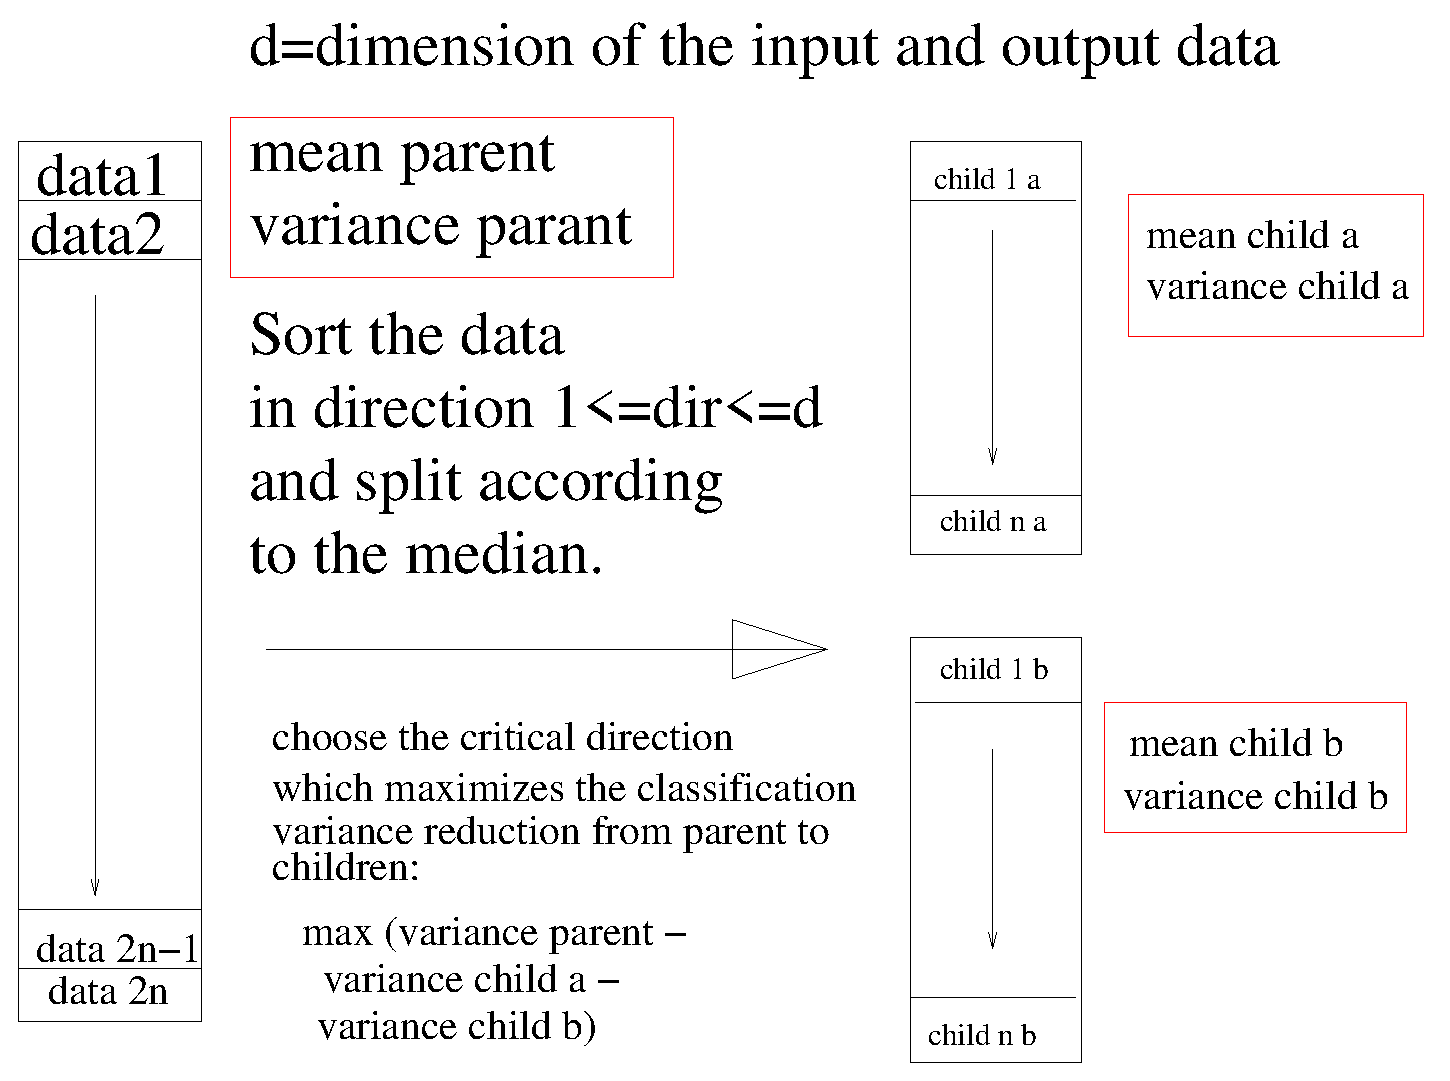
\includegraphics[width=0.8\textwidth]{DT_figure.eps}
\caption{Illustration of regression decision tree 
 splitting\cite{breiman1984classification}\label{DT_figure} for 
 predicting the slope of the CMOF (or MOF) reconstructed interface
 given the reference centroid and volume fraction.}
\end{figure}


\subsection{Reconstructing the distance function \label{MMRECON}}
Here we describe a distance function reconstruction algorithm that evaluate the exact signed distance function to the reconstructed interface.

Assuming that the reconstructed interface is available on the multimaterial cells, using a MOF or CMOF reconstruction, the algorithm first initialize the distance function to a large number with correct sign. Then in a narrow band the cells tagged for involvement in the redistancing procedure, that is, contributing information to and/or getting updated distance function value through this process. In the next steps, distances are evaluated from the center of an update cell to different possible interfacial points in its neighborhood, and material, $\phi_m$, and interface distance functions ,$\phi_{m1,m2}$, are updated consequently.

\begin{itemize}
\item Set all distance functions, $\phi_m$ and $\phi_{m1,m2}$, 
to a large negative value.
\item Iterate over all cells.  
  \begin{itemize}
  \item Using the reconstructed interface, change the sign of 
    $\phi_k$ and $\phi_{k,m2}$ to positive if material 
    $k$ is occupying the
    center of a cell.
  \item For a cell, check the neighbors for 
    occupying materials in a  $3 \times 3 \times 3$ 
    hypercube stencil around it. Count the
    materials $m$ present if $F_m>0.5$ in at 
    least one of the cells in the stencil, or if a 
    material level set changes sign between two 
    different cells in the stencil. If more than one 
    material are present in the stencil, this cell is 
    a \emph{support} cell for the redistancing 
    algorithm. Consequently, tag cells in the $9 \times 9 \times 9$ 
    hypercube around a support cell as \emph{update} cells.
 \end{itemize}
 \item Iterate over update cells.
   \begin{itemize}
   \item Iterate over the support cells in the $3 \times 3 \times 3$  
    hypercube around this update cell. 
     \begin{itemize}
     \item Evaluate distance to the corners, face centers, and 
      cell center in the support cell. This procedure gives 
      the exact distance if cell boundaries are 
      part of the material interface (Figure \ref{fig:redistancing}.a).
     \item Find the normal distance to each interface in the 
      support cell. Update the distance only if the 
      intersection point is within the support cell 
      (Figure \ref{fig:redistancing}.b).
     \item Find the intersection of each pair of the interfaces 
      in the support cell, and evaluate the distance 
      to the triple-point. Check the materials around the 
      intersection for updating the corresponding interface 
      distance functions (Figure \ref{fig:redistancing}.c).
     \item Find the intersection of the interfaces with 
      cell faces, evaluate the distance, and update the 
      corresponding distance functions (Figure \ref{fig:redistancing}.d).
     \item For 3D cases only, find the intersection line of 
       each pair of interfacial planes, and find the intersection 
      of the cell boundaries with the line. 
      Then, evaluate the distance to the intersection points, and update the corresponding distance functions (Figure \ref{fig:redistancing_3D}).
     \end{itemize}
   \end{itemize}
\end{itemize}

Notes:
\begin{itemize}
\item[-] In the redistancing algorithm, 
  after finding the distance to an interface or intersection of 
  interface with cell boundaries or other interfaces the 
  materials around the intersection points are found by 
  testing some points around the intersection to figure out 
  which material they belong to. These points are 
  picked by the combination of interface normal vectors 
  involved in the intersection points and are shown with white 
  diamonds in Figure \ref{fig:redistancing} and 
  Figure \ref{fig:redistancing_3D}.
\item[-] Both distance function value and normal vector is 
 updated if a distance measurement is found with smaller 
 magnitude compared to the stored value in $\phi_{m}$ and $\phi_{m1,m2}$.
\item[-] Applying the algorithm described above, an interface 
 distance function $\phi_{m1,m2}$ is not well defined when the 
 update cell belongs to neither material $m1$ nor 
 material $m2$ (Figure \ref{fig:redistancing_ils}.a). 
 An alternative measurement is used to extend the 
 interface distance functions (Figure \ref{fig:redistancing_ils}.b). 
 For a cell $\{i,j\}$ where $\phi_{m1,i,j}<0$ and $\phi_{m2,i,j}<0$ we have:
  \begin{eqnarray}
    \bmx_{m1} &=& \bmx_{i,j} - \phi_{m1,i,j} \bmn_{m1,i,j}, \\
    \bmx_{m2} &=& \bmx_{i,j} - \phi_{m2,i,j} \bmn_{m2,i,j}, \\
    \bmq &=& \bmx_{m1} - \bmx_{m2}.
  \end{eqnarray}
  \begin{equation}
    \left\{
      \begin{array}{lll}
        \phi_{m1,m2} = |\bmq|  &\tn{if } |\phi_{m1,i,j}| < |\phi_{m2,i,j}| \\
        \phi_{m1,m2} = -|\bmq| &\tn{if } |\phi_{m1,i,j}| \ge |\phi_{m2,i,j}| \\
      \end{array}
    \right.
  \end{equation}
\end{itemize}
 
\begin{figure}[htbp]
  \centering
  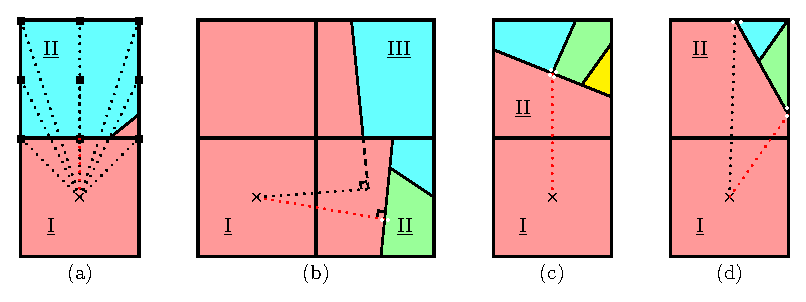
\includegraphics[width=0.8\textwidth]{redistancing.eps}
%%  \scalebox{0.85}
%%  { %%Created by jPicEdt 1.4.1_03: mixed JPIC-XML/LaTeX format
%%Mon Jul 25 14:16:56 EDT 2016
%%Begin JPIC-XML
%<?xml version="1.0" standalone="yes"?>
%<jpic x-min="0" x-max="130" y-min="-3" y-max="40" auto-bounding="true">
%<multicurve fill-style= "solid"
%	 stroke-style= "none"
%	 points= "(130,40);(130,40);(125,33);(125,33);(125,33);(130,24);
%	(130,24);(130,24);(130,40)"
%	 pstcustom= "opacity=0.5"
%	 fill-color= "#99ff99"
%	 />
%<multicurve fill-style= "solid"
%	 points= "(30,40);(30,40);(56,40);(56,40);(56,40);(58,20);
%	(58,20);(58,20);(63,20);(63,20);(63,20);(61,0);
%	(61,0);(61,0);(30,0);(30,0);(30,0);(30,40)"
%	 pstcustom= "opacity=0.5"
%	 fill-color= "#ff9999"
%	 />
%<multicurve fill-style= "solid"
%	 points= "(80,-0);(80,-0);(80,20);(80,20);(80,20);(80,28);
%	(80,28);(80,28);(80,35);(80,35);(80,35);(100,27);
%	(100,27);(100,27);(100,0);(100,0);(100,0);(80,-0)"
%	 pstcustom= "opacity=0.5"
%	 fill-color= "#ff9999"
%	 />
%<multicurve fill-style= "solid"
%	 points= "(90,31);(90,31);(95,29);(95,29);(95,29);(100,36);
%	(100,36);(100,36);(100,40);(100,40);(100,40);(94,40);
%	(94,40);(94,40);(90,31)"
%	 pstcustom= "opacity=0.5"
%	 fill-color= "#99ff99"
%	 />
%<multicurve fill-style= "solid"
%	 points= "(62.5,15);(62.5,15);(61,0);(61,0);(61,0);(70,0);
%	(70,0);(70,0);(70,10);(70,10);(70,10);(62.5,15)"
%	 pstcustom= "opacity=0.5"
%	 fill-color= "#99ff99"
%	 />
%<multicurve fill-style= "solid"
%	 points= "(0,20);(0,20);(15,20);(15,20);(15,20);(20,24);
%	(20,24);(20,24);(20,0);(20,0);(20,0);(0,0);
%	(0,0);(0,0);(0,20)"
%	 pstcustom= "opacity=0.5"
%	 fill-color= "#ff9999"
%	 />
%<multicurve fill-style= "solid"
%	 points= "(0,40);(0,40);(0,20);(0,20);(0,20);(15,20);
%	(15,20);(15,20);(20,24);(20,24);(20,24);(20,40);
%	(20,40);(20,40);(0,40)"
%	 pstcustom= "opacity=0.5"
%	 fill-color= "#66ffff"
%	 />
%<text text-vert-align= "center-v"
%	 fill-style= "none"
%	 anchor-point= "(5,5)"
%	 text-frame= "noframe"
%	 text-hor-align= "center-h"
%	 >
%\underline{I}
%</text>
%<text text-vert-align= "center-v"
%	 fill-style= "none"
%	 anchor-point= "(5,35)"
%	 text-frame= "noframe"
%	 text-hor-align= "center-h"
%	 >
%\underline{II}
%</text>
%<multicurve fill-style= "none"
%	 stroke-style= "dotted"
%	 points= "(10,10);(10,10);(0,20);(0,20)"
%	 />
%<multicurve fill-style= "none"
%	 stroke-style= "dotted"
%	 points= "(10,10);(10,10);(0,30);(0,30)"
%	 />
%<multicurve fill-style= "none"
%	 stroke-style= "dotted"
%	 points= "(10,10);(10,10);(0,40);(0,40)"
%	 />
%<multicurve fill-style= "none"
%	 stroke-style= "dotted"
%	 points= "(10,10);(10,10);(10,40);(10,40)"
%	 />
%<multicurve fill-style= "none"
%	 stroke-style= "dotted"
%	 points= "(10,10);(10,10);(20,40);(20,40)"
%	 />
%<multicurve fill-style= "none"
%	 stroke-style= "dotted"
%	 points= "(10,10);(10,10);(20,30);(20,30)"
%	 />
%<multicurve fill-style= "none"
%	 stroke-style= "dotted"
%	 points= "(10,10);(10,10);(20,20);(20,20)"
%	 />
%<parallelogram p3= "(20,0)"
%	 p2= "(20,20)"
%	 p1= "(0,20)"
%	 fill-style= "none"
%	 stroke-width= "0.4"
%	 />
%<multicurve polydots-scale-v= "1"
%	 polydots-superimpose= "false"
%	 polydots-style= "polydots-square-filled"
%	 fill-style= "none"
%	 polydots-angle= "0"
%	 polydots-size-minimum= "0.7"
%	 points= "(10,40);(10,40);(0,40);(0,40);(0,40);(20,40);
%	(20,40);(20,40);(10,30);(10,30);(10,30);(20,30);
%	(20,30);(20,30);(20,20);(20,20);(20,20);(10,20);
%	(10,20);(10,20);(0,20);(0,20);(0,20);(0,30);
%	(0,30)"
%	 polydots-scale-h= "1"
%	 polydots-size-linewidth-scale= "1.5"
%	 />
%<parallelogram p3= "(20,20)"
%	 p2= "(20,40)"
%	 p1= "(0,40)"
%	 fill-style= "none"
%	 stroke-width= "0.4"
%	 />
%<text text-vert-align= "center-v"
%	 fill-style= "none"
%	 anchor-point= "(10,-3)"
%	 text-frame= "noframe"
%	 text-hor-align= "center-h"
%	 >
%(a)
%</text>
%<multicurve fill-style= "none"
%	 stroke-style= "dotted"
%	 points= "(10,10);(10,10);(10,30);(10,30)"
%	 />
%<multicurve fill-style= "none"
%	 stroke-style= "dotted"
%	 points= "(10,10);(10,10);(10,20);(10,20)"
%	 stroke-color= "#ff0000"
%	 />
%<multicurve fill-style= "solid"
%	 points= "(56,40);(56,40);(58,20);(58,20);(58,20);(63,20);
%	(63,20);(63,20);(62.5,15);(62.5,15);(62.5,15);(70,10);
%	(70,10);(70,10);(70,40);(70,40);(70,40);(56,40)"
%	 pstcustom= "opacity=0.5"
%	 fill-color= "#66ffff"
%	 />
%<text text-vert-align= "center-v"
%	 fill-style= "none"
%	 anchor-point= "(35,5)"
%	 text-frame= "noframe"
%	 text-hor-align= "center-h"
%	 >
%\underline{I}
%</text>
%<text text-vert-align= "center-v"
%	 fill-style= "none"
%	 anchor-point= "(65,5)"
%	 text-frame= "noframe"
%	 text-hor-align= "center-h"
%	 >
%\underline{II}
%</text>
%<parallelogram p3= "(50,0)"
%	 p2= "(50,20)"
%	 p1= "(30,20)"
%	 fill-style= "none"
%	 stroke-width= "0.4"
%	 />
%<parallelogram p3= "(50,20)"
%	 p2= "(50,40)"
%	 p1= "(30,40)"
%	 fill-style= "none"
%	 stroke-width= "0.4"
%	 />
%<text text-vert-align= "center-v"
%	 fill-style= "none"
%	 anchor-point= "(50,-3)"
%	 text-frame= "noframe"
%	 text-hor-align= "center-h"
%	 >
%(b)
%</text>
%<parallelogram p3= "(70,20)"
%	 p2= "(70,40)"
%	 p1= "(50,40)"
%	 fill-style= "none"
%	 stroke-width= "0.4"
%	 />
%<parallelogram p3= "(70,0)"
%	 p2= "(70,20)"
%	 p1= "(50,20)"
%	 fill-style= "none"
%	 stroke-width= "0.4"
%	 />
%<text text-vert-align= "center-v"
%	 fill-style= "none"
%	 anchor-point= "(64,35)"
%	 text-frame= "noframe"
%	 text-hor-align= "center-h"
%	 >
%\underline{III}
%</text>
%<multicurve fill-style= "none"
%	 stroke-style= "dotted"
%	 points= "(40,10);(40,10);(61.64,6.25);(61.64,6.25)"
%	 stroke-color= "#ff0000"
%	 />
%<multicurve fill-style= "none"
%	 stroke-dasharray= "1;1"
%	 stroke-style= "dashed"
%	 points= "(58.85,11.41);(58.85,11.41);(56,40);(56,40)"
%	 />
%<multicurve fill-style= "none"
%	 stroke-style= "dotted"
%	 points= "(40,10);(40,10);(58.65,11.35);(58.65,11.35)"
%	 />
%<multicurve fill-style= "none"
%	 points= "(60.4,6.71);(60.4,6.71);(60.55,7.7);(60.55,7.7);(60.55,7.7);(61.54,7.55);
%	(61.54,7.55)"
%	 />
%<multicurve fill-style= "none"
%	 points= "(57.64,11.51);(57.64,11.51);(57.55,12.51);(57.55,12.51);(57.55,12.51);(58.54,12.6);
%	(58.54,12.6)"
%	 />
%<multicurve polydots-scale-v= "1"
%	 polydots-superimpose= "false"
%	 polydots-style= "polydots-square-filled"
%	 fill-style= "none"
%	 polydots-angle= "45"
%	 polydots-size-minimum= "0.5"
%	 points= "(62.11,6.15);(62.11,6.15);(61.15,6.25);(61.15,6.25)"
%	 polydots-scale-h= "1"
%	 polydots-size-linewidth-scale= "0.1"
%	 stroke-color= "#ffffff"
%	 />
%<multicurve fill-style= "solid"
%	 points= "(80,35);(80,35);(80,35);(80,35);(80,35);(80,35);
%	(80,35);(80,35);(90,31);(90,31);(90,31);(94,40);
%	(94,40);(94,40);(80,40);(80,40);(80,40);(80,35)"
%	 pstcustom= "opacity=0.5"
%	 fill-color= "#66ffff"
%	 />
%<text text-vert-align= "center-v"
%	 fill-style= "none"
%	 anchor-point= "(85,5)"
%	 text-frame= "noframe"
%	 text-hor-align= "center-h"
%	 >
%\underline{I}
%</text>
%<text text-vert-align= "center-v"
%	 fill-style= "none"
%	 anchor-point= "(85,25)"
%	 text-frame= "noframe"
%	 text-hor-align= "center-h"
%	 >
%\underline{II}
%</text>
%<parallelogram p3= "(100,20)"
%	 p2= "(80,20)"
%	 p1= "(80,-0)"
%	 fill-style= "none"
%	 stroke-width= "0.4"
%	 />
%<text text-vert-align= "center-v"
%	 fill-style= "none"
%	 anchor-point= "(90,-3)"
%	 text-frame= "noframe"
%	 text-hor-align= "center-h"
%	 >
%(c)
%</text>
%<parallelogram p3= "(100,40)"
%	 p2= "(80,40)"
%	 p1= "(80,20)"
%	 fill-style= "none"
%	 stroke-width= "0.4"
%	 />
%<multicurve fill-style= "none"
%	 stroke-style= "dotted"
%	 points= "(90,10);(90,10);(90,31);(90,31)"
%	 stroke-color= "#ff0000"
%	 />
%<multicurve polydots-scale-v= "1"
%	 polydots-superimpose= "false"
%	 polydots-style= "polydots-square-filled"
%	 fill-style= "none"
%	 polydots-angle= "45"
%	 polydots-size-minimum= "0.5"
%	 points= "(90.57,31.23);(90.57,31.23);(89.46,30.74);(89.46,30.74);(89.46,30.74);(90.25,30.43);
%	(90.25,30.43);(90.25,30.43);(89.75,31.58);(89.75,31.58)"
%	 polydots-scale-h= "1"
%	 polydots-size-linewidth-scale= "0.1"
%	 stroke-color= "#ffffff"
%	 />
%<multicurve fill-style= "solid"
%	 points= "(95,29);(95,29);(100,27);(100,27);(100,27);(100,36);
%	(100,36);(100,36);(95,29)"
%	 pstcustom= "opacity=0.5"
%	 fill-color= "#ffff00"
%	 />
%<multicurve fill-style= "solid"
%	 points= "(110,40);(110,40);(121,40);(121,40);(121,40);(130,24);
%	(130,24);(130,24);(130,0);(130,0);(130,0);(110,0);
%	(110,0);(110,0);(110,40)"
%	 pstcustom= "opacity=0.5"
%	 fill-color= "#ff9999"
%	 />
%<multicurve fill-style= "solid"
%	 points= "(121,40);(121,40);(125,33);(125,33);(125,33);(129.9,39.98);
%	(129.9,39.98);(129.9,39.98);(121,40)"
%	 pstcustom= "opacity=0.5"
%	 fill-color= "#66ffff"
%	 />
%<text text-vert-align= "center-v"
%	 fill-style= "none"
%	 anchor-point= "(115,5)"
%	 text-frame= "noframe"
%	 text-hor-align= "center-h"
%	 >
%\underline{I}
%</text>
%<text text-vert-align= "center-v"
%	 fill-style= "none"
%	 anchor-point= "(115,35)"
%	 text-frame= "noframe"
%	 text-hor-align= "center-h"
%	 >
%\underline{II}
%</text>
%<multicurve fill-style= "none"
%	 stroke-style= "dotted"
%	 points= "(120,10);(120,10);(121,40);(121,40)"
%	 />
%<parallelogram p3= "(130,0)"
%	 p2= "(130,20)"
%	 p1= "(110,20)"
%	 fill-style= "none"
%	 stroke-width= "0.4"
%	 />
%<parallelogram p3= "(130,20)"
%	 p2= "(130,40)"
%	 p1= "(110,40)"
%	 fill-style= "none"
%	 stroke-width= "0.4"
%	 />
%<text text-vert-align= "center-v"
%	 fill-style= "none"
%	 anchor-point= "(120,-3)"
%	 text-frame= "noframe"
%	 text-hor-align= "center-h"
%	 >
%(d)
%</text>
%<multicurve polydots-scale-v= "1"
%	 polydots-superimpose= "false"
%	 polydots-style= "polydots-plus"
%	 fill-style= "none"
%	 polydots-angle= "45"
%	 polydots-size-minimum= "0.7"
%	 points= "(120,10);(120,10);(10,10);(10,10);(10,10);(90,10);
%	(90,10);(90,10);(40,10);(40,10)"
%	 polydots-scale-h= "1"
%	 polydots-size-linewidth-scale= "3.5"
%	 />
%<multicurve fill-style= "none"
%	 stroke-style= "dotted"
%	 points= "(120,10);(120,10);(130,24);(130,24)"
%	 stroke-color= "#ff0000"
%	 />
%<multicurve polydots-scale-v= "1"
%	 polydots-superimpose= "false"
%	 polydots-style= "polydots-square-filled"
%	 fill-style= "none"
%	 polydots-angle= "45"
%	 polydots-size-minimum= "0.5"
%	 points= "(129.7,23.78);(129.7,23.78);(129.72,25.13);(129.72,25.13)"
%	 polydots-scale-h= "1"
%	 polydots-size-linewidth-scale= "0.1"
%	 stroke-color= "#ffffff"
%	 />
%<multicurve polydots-scale-v= "1"
%	 polydots-superimpose= "false"
%	 polydots-style= "polydots-square-filled"
%	 fill-style= "none"
%	 polydots-angle= "45"
%	 polydots-size-minimum= "0.5"
%	 points= "(121.86,39.68);(121.86,39.68);(120.51,39.68);(120.51,39.68)"
%	 polydots-scale-h= "1"
%	 polydots-size-linewidth-scale= "0.1"
%	 stroke-color= "#ffffff"
%	 />
%</jpic>
%%End JPIC-XML
%PSTricks content-type (pstricks.sty package needed)
%Add \usepackage{pstricks} in the preamble of your LaTeX file
%You can rescale the whole picture (to 80% for instance) by using the command \def\JPicScale{0.8}
\ifx\JPicScale\undefined\def\JPicScale{1}\fi
\psset{unit=\JPicScale mm}
\psset{linewidth=0.3,dotsep=1,hatchwidth=0.3,hatchsep=1.5,shadowsize=1,dimen=middle}
\psset{dotsize=0.7 2.5,dotscale=1 1,fillcolor=black}
\psset{arrowsize=1 2,arrowlength=1,arrowinset=0.25,tbarsize=0.7 5,bracketlength=0.15,rbracketlength=0.15}
\begin{pspicture}(0,0)(130,40)
\newrgbcolor{userFillColour}{0.6 1 0.6}
\pspolygon[linestyle=none,fillcolor=userFillColour,fillstyle=solid,opacity=0.5](130,40)
(125,33)
(130,24)(130,40)
\newrgbcolor{userFillColour}{1 0.6 0.6}
\pspolygon[fillcolor=userFillColour,fillstyle=solid,opacity=0.5](30,40)
(56,40)
(58,20)
(63,20)
(61,0)
(30,0)(30,40)
\newrgbcolor{userFillColour}{1 0.6 0.6}
\pspolygon[fillcolor=userFillColour,fillstyle=solid,opacity=0.5](80,-0)
(80,20)
(80,28)
(80,35)
(100,27)
(100,0)(80,-0)
\newrgbcolor{userFillColour}{0.6 1 0.6}
\pspolygon[fillcolor=userFillColour,fillstyle=solid,opacity=0.5](90,31)
(95,29)
(100,36)
(100,40)
(94,40)(90,31)
\newrgbcolor{userFillColour}{0.6 1 0.6}
\pspolygon[fillcolor=userFillColour,fillstyle=solid,opacity=0.5](62.5,15)
(61,0)
(70,0)
(70,10)(62.5,15)
\newrgbcolor{userFillColour}{1 0.6 0.6}
\pspolygon[fillcolor=userFillColour,fillstyle=solid,opacity=0.5](0,20)
(15,20)
(20,24)
(20,0)
(0,0)(0,20)
\newrgbcolor{userFillColour}{0.4 1 1}
\pspolygon[fillcolor=userFillColour,fillstyle=solid,opacity=0.5](0,40)
(0,20)
(15,20)
(20,24)
(20,40)(0,40)
\rput(5,5){\underline{I}}
\rput(5,35){\underline{II}}
\psline[linestyle=dotted](10,10)(0,20)
\psline[linestyle=dotted](10,10)(0,30)
\psline[linestyle=dotted](10,10)(0,40)
\psline[linestyle=dotted](10,10)(10,40)
\psline[linestyle=dotted](10,10)(20,40)
\psline[linestyle=dotted](10,10)(20,30)
\psline[linestyle=dotted](10,10)(20,20)
\pspolygon[linewidth=0.4](0,20)(20,20)(20,0)(0,0)
\psdots[dotsize=0.7 1.5,dotstyle=square*](10,40)
(0,40)(20,40)(10,30)(20,30)(20,20)(10,20)(0,20)(0,30)
\pspolygon[linewidth=0.4](0,40)(20,40)(20,20)(0,20)
\rput(10,-3){(a)}
\psline[linestyle=dotted](10,10)(10,30)
\psline[linecolor=red,linestyle=dotted](10,10)(10,20)
\newrgbcolor{userFillColour}{0.4 1 1}
\pspolygon[fillcolor=userFillColour,fillstyle=solid,opacity=0.5](56,40)
(58,20)
(63,20)
(62.5,15)
(70,10)
(70,40)(56,40)
\rput(35,5){\underline{I}}
\rput(65,5){\underline{II}}
\pspolygon[linewidth=0.4](30,20)(50,20)(50,0)(30,0)
\pspolygon[linewidth=0.4](30,40)(50,40)(50,20)(30,20)
\rput(50,-3){(b)}
\pspolygon[linewidth=0.4](50,40)(70,40)(70,20)(50,20)
\pspolygon[linewidth=0.4](50,20)(70,20)(70,0)(50,0)
\rput(64,35){\underline{III}}
\psline[linecolor=red,linestyle=dotted](40,10)(61.64,6.25)
\psline[linestyle=dashed,dash=1 1](58.85,11.41)(56,40)
\psline[linestyle=dotted](40,10)(58.65,11.35)
\psline(60.4,6.71)
(60.55,7.7)(61.54,7.55)
\psline(57.64,11.51)
(57.55,12.51)(58.54,12.6)
\psdots[linecolor=white,dotsize=0.5 0.1,dotstyle=square*,dotangle=45](62.11,6.15)
(61.15,6.25)
\newrgbcolor{userFillColour}{0.4 1 1}
\pscustom[fillcolor=userFillColour,fillstyle=solid,opacity=0.5]{\psbezier(80,35)(80,35)(80,35)(80,35)
\psbezier(80,35)(80,35)(80,35)
\psline(80,35)(90,31)
\psline(90,31)(94,40)
\psline(94,40)(80,40)
\psline(80,40)(80,35)
\closepath}
\rput(85,5){\underline{I}}
\rput(85,25){\underline{II}}
\pspolygon[linewidth=0.4](80,-0)(80,20)(100,20)(100,0)
\rput(90,-3){(c)}
\pspolygon[linewidth=0.4](80,20)(80,40)(100,40)(100,20)
\psline[linecolor=red,linestyle=dotted](90,10)(90,31)
\psdots[linecolor=white,dotsize=0.5 0.1,dotstyle=square*,dotangle=45](90.57,31.23)
(89.46,30.74)(90.25,30.43)(89.75,31.58)
\pspolygon[fillcolor=yellow,fillstyle=solid,opacity=0.5](95,29)
(100,27)
(100,36)(95,29)
\newrgbcolor{userFillColour}{1 0.6 0.6}
\pspolygon[fillcolor=userFillColour,fillstyle=solid,opacity=0.5](110,40)
(121,40)
(130,24)
(130,0)
(110,0)(110,40)
\newrgbcolor{userFillColour}{0.4 1 1}
\pspolygon[fillcolor=userFillColour,fillstyle=solid,opacity=0.5](121,40)
(125,33)
(129.9,39.98)(121,40)
\rput(115,5){\underline{I}}
\rput(115,35){\underline{II}}
\psline[linestyle=dotted](120,10)(121,40)
\pspolygon[linewidth=0.4](110,20)(130,20)(130,0)(110,0)
\pspolygon[linewidth=0.4](110,40)(130,40)(130,20)(110,20)
\rput(120,-3){(d)}
\psdots[dotsize=0.7 3.5,dotstyle=+,dotangle=45](120,10)
(10,10)(90,10)(40,10)
\psline[linecolor=red,linestyle=dotted](120,10)(130,24)
\psdots[linecolor=white,dotsize=0.5 0.1,dotstyle=square*,dotangle=45](129.7,23.78)
(129.72,25.13)
\psdots[linecolor=white,dotsize=0.5 0.1,dotstyle=square*,dotangle=45](121.86,39.68)
(120.51,39.68)
\end{pspicture}
 }
  \caption{Redistancing procedures:(a) Update cell I, support cell II, distances are measured to the corners, face centers, and cell center in the support cell (dotted lines). Here, the distance to the bottom face center (red dotted line) is the true distance to the interface between two materials. (b) Update cell I, support cell II, normal distances (red dotted lines) is measured to the first interface. Since the intersection point is within the cell II, two materials around the interface is found using the testing points (white diamonds). Here, the signed distance and normal vector for the red and green material distance function and the red-green interface distance function are updated. However, when the case for update cell I and support cell III is considered, the normal distances (black dotted lines) is measured to the interface, and the intersection point is outside of cell III. Therefore, this measurement is not considered for redistancing update. (c) Update cell I, support cell II, the distance to the intersection of the first and second interfaces is measured (red dotted lines). The three materials around the triple-point is found checking the testing points (white diamonds). Here, the red, blue, and green material distance functions, and the red-blue, red-green, and blue-green interface distance functions are updated. (d) Update cell I, support cell II, distances to the intersection of the first interface with cell faces are measured (dotted lines). Here, for the red dotted line measurement, the red and green material distance functions, and the red-green interface distance functions are updated.}
  \label{fig:redistancing}
\end{figure}

\begin{figure}[htbp]
  \centering
  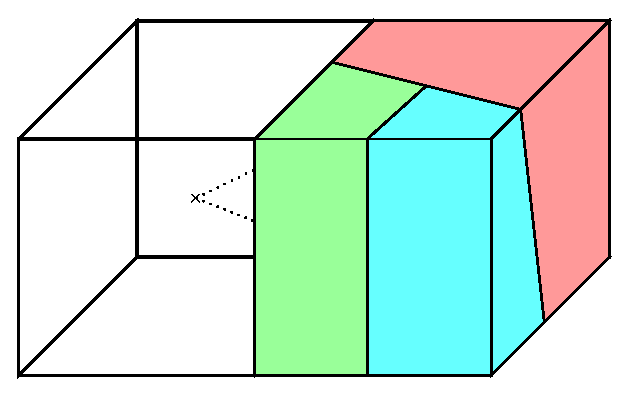
\includegraphics[width=0.8\textwidth]{redistancing_3D.eps}
%%  \scalebox{0.8}
%%  { %%Created by jPicEdt 1.4.1_03: mixed JPIC-XML/LaTeX format
%%Mon Jul 25 13:05:42 EDT 2016
%%Begin JPIC-XML
%<?xml version="1.0" standalone="yes"?>
%<jpic x-min="0" x-max="100" y-min="0" y-max="60" auto-bounding="true">
%<multicurve fill-style= "solid"
%	 points= "(60,60);(60,60);(60,20);(60,20);(60,20);(57,17);
%	(57,17);(57,17);(53,53);(53,53);(53,53);(60,60)"
%	 pstcustom= "opacity=0.5"
%	 fill-color= "#ff9999"
%	 />
%<multicurve fill-style= "solid"
%	 points= "(60,60);(60,60);(100,60);(100,60);(100,60);(100,20);
%	(100,20);(100,20);(60,20);(60,20);(60,20);(60,60)"
%	 pstcustom= "opacity=0.5"
%	 fill-color= "#ff9999"
%	 />
%<parallelogram p3= "(60,20)"
%	 p2= "(60,60)"
%	 p1= "(20,60)"
%	 fill-style= "none"
%	 stroke-width= "0.4"
%	 />
%<multicurve fill-style= "solid"
%	 points= "(60,20);(60,20);(100,20);(100,20);(100,20);(89,9);
%	(89,9);(89,9);(57,17);(57,17);(57,17);(60,20)"
%	 pstcustom= "opacity=0.5"
%	 fill-color= "#ff9999"
%	 />
%<multicurve fill-style= "none"
%	 stroke-width= "0.4"
%	 points= "(60,60);(60,60);(100,60);(100,60);(100,60);(100,20);
%	(100,20);(100,20);(60,20);(60,20);(60,20);(60,60)"
%	 />
%<multicurve polydots-scale-v= "1"
%	 polydots-superimpose= "false"
%	 polydots-style= "polydots-square-filled"
%	 fill-style= "none"
%	 polydots-angle= "45"
%	 polydots-size-minimum= "0.5"
%	 points= "(73.85,13.55);(73.85,13.55);(69.9,49.47);(69.9,49.47)"
%	 polydots-scale-h= "1"
%	 polydots-size-linewidth-scale= "0.1"
%	 stroke-color= "#ffffff"
%	 />
%<multicurve polydots-scale-v= "1"
%	 polydots-superimpose= "false"
%	 polydots-style= "polydots-square-filled"
%	 fill-style= "none"
%	 polydots-angle= "45"
%	 polydots-size-minimum= "0.5"
%	 points= "(72.8,13.68);(72.8,13.68);(68.36,49.67);(68.36,49.67)"
%	 polydots-scale-h= "1"
%	 polydots-size-linewidth-scale= "0.1"
%	 stroke-color= "#ffffff"
%	 />
%<multicurve fill-style= "solid"
%	 points= "(60,60);(60,60);(100,60);(100,60);(100,60);(85,45);
%	(85,45);(85,45);(53,53);(53,53);(53,53);(60,60)"
%	 pstcustom= "opacity=0.5"
%	 fill-color= "#ff9999"
%	 />
%<multicurve fill-style= "solid"
%	 stroke-style= "none"
%	 points= "(53,53);(53,53);(57,17);(57,17);(57,17);(89,9);
%	(89,9);(89,9);(85,45);(85,45);(85,45);(53,53)"
%	 pstcustom= "opacity=0.5"
%	 fill-color= "#c0c0c0"
%	 />
%<multicurve fill-style= "solid"
%	 points= "(57,17);(57,17);(40,0);(40,0);(40,0);(59,0);
%	(59,0);(59,0);(73,13);(73,13);(73,13);(57,17)"
%	 pstcustom= "opacity=0.5"
%	 fill-color= "#99ff99"
%	 />
%<multicurve fill-style= "none"
%	 stroke-style= "dotted"
%	 points= "(30,30);(30,30);(49.23,22.4);(49.23,22.4)"
%	 />
%<multicurve fill-style= "none"
%	 stroke-style= "dotted"
%	 points= "(30,30);(30,30);(49.33,39.39);(49.33,39.39)"
%	 />
%<multicurve fill-style= "solid"
%	 points= "(40,40);(40,40);(40,0);(40,0);(40,0);(57,17);
%	(57,17);(57,17);(53,53);(53,53);(53,53);(40,40)"
%	 pstcustom= "opacity=0.5"
%	 fill-color= "#99ff99"
%	 />
%<multicurve polydots-scale-v= "1"
%	 polydots-superimpose= "false"
%	 polydots-style= "polydots-square-filled"
%	 fill-style= "none"
%	 polydots-angle= "45"
%	 polydots-size-minimum= "0.5"
%	 points= "(71.94,12.99);(71.94,12.99);(67.93,48.75);(67.93,48.75)"
%	 polydots-scale-h= "1"
%	 polydots-size-linewidth-scale= "0.1"
%	 stroke-color= "#ffffff"
%	 />
%<multicurve fill-style= "none"
%	 stroke-style= "dotted"
%	 points= "(50.02,22.09);(50.02,22.09);(73,13);(73,13)"
%	 />
%<multicurve fill-style= "solid"
%	 stroke-style= "none"
%	 points= "(59,40);(59,40);(59,0);(59,0);(59,0);(73,13);
%	(73,13);(73,13);(69,49);(69,49);(69,49);(59,40)"
%	 pstcustom= "opacity=0.5"
%	 fill-color= "#808080"
%	 />
%<multicurve fill-style= "solid"
%	 points= "(73,13);(73,13);(59,0);(59,0);(59,0);(80,0);
%	(80,0);(80,0);(89,9);(89,9);(89,9);(73,13)"
%	 pstcustom= "opacity=0.5"
%	 fill-color= "#66ffff"
%	 />
%<multicurve fill-style= "none"
%	 stroke-dasharray= "1;1"
%	 stroke-style= "dashed"
%	 points= "(69,49);(69,49);(73,13);(73,13)"
%	 />
%<multicurve polydots-scale-v= "1"
%	 polydots-superimpose= "false"
%	 polydots-style= "polydots-square-filled"
%	 fill-style= "none"
%	 polydots-angle= "45"
%	 polydots-size-minimum= "0.5"
%	 points= "(73.09,12.63);(73.09,12.63);(69.28,48.31);(69.28,48.31)"
%	 polydots-scale-h= "1"
%	 polydots-size-linewidth-scale= "0.1"
%	 stroke-color= "#ffffff"
%	 />
%<parallelogram p3= "(40,0)"
%	 p2= "(40,40)"
%	 p1= "(0,40)"
%	 fill-style= "none"
%	 stroke-width= "0.4"
%	 />
%<parallelogram p3= "(20,20)"
%	 p2= "(20,60)"
%	 p1= "(0,40)"
%	 fill-style= "none"
%	 stroke-width= "0.4"
%	 />
%<multicurve polydots-scale-v= "1"
%	 polydots-superimpose= "false"
%	 polydots-style= "polydots-plus"
%	 fill-style= "none"
%	 polydots-angle= "45"
%	 polydots-size-minimum= "0.7"
%	 points= "(30,30);(30,30);(30,30);(30,30)"
%	 polydots-scale-h= "1"
%	 polydots-size-linewidth-scale= "3.5"
%	 />
%<parallelogram p3= "(80,0)"
%	 p2= "(80,40)"
%	 p1= "(40,40)"
%	 fill-style= "none"
%	 stroke-width= "0.4"
%	 />
%<multicurve fill-style= "none"
%	 stroke-style= "dotted"
%	 points= "(50.16,39.82);(50.16,39.82);(68.92,49.02);(68.92,49.02)"
%	 />
%<multicurve fill-style= "solid"
%	 points= "(53,53);(53,53);(40,40);(40,40);(40,40);(59,40);
%	(59,40);(59,40);(69,49);(69,49);(69,49);(53,53)"
%	 pstcustom= "opacity=0.5"
%	 fill-color= "#99ff99"
%	 />
%<multicurve fill-style= "solid"
%	 points= "(40,40);(40,40);(40,0);(40,0);(40,0);(59,0);
%	(59,0);(59,0);(59,40);(59,40);(59,40);(40,40)"
%	 pstcustom= "opacity=0.5"
%	 fill-color= "#99ff99"
%	 />
%<multicurve fill-style= "solid"
%	 points= "(69,49);(69,49);(59,40);(59,40);(59,40);(80,40);
%	(80,40);(80,40);(85,45);(85,45);(85,45);(69,49)"
%	 pstcustom= "opacity=0.5"
%	 fill-color= "#66ffff"
%	 />
%<multicurve fill-style= "solid"
%	 points= "(59,40);(59,40);(59,0);(59,0);(59,0);(80,0);
%	(80,0);(80,0);(80,40);(80,40);(80,40);(59,40)"
%	 pstcustom= "opacity=0.5"
%	 fill-color= "#66ffff"
%	 />
%<multicurve fill-style= "solid"
%	 points= "(100,60);(100,60);(100,20);(100,20);(100,20);(89,9);
%	(89,9);(89,9);(85,45);(85,45);(85,45);(100,60)"
%	 pstcustom= "opacity=0.5"
%	 fill-color= "#ff9999"
%	 />
%<multicurve fill-style= "solid"
%	 points= "(80,40);(80,40);(80,0);(80,0);(80,0);(89,9);
%	(89,9);(89,9);(85,45);(85,45);(85,45);(80,40)"
%	 pstcustom= "opacity=0.5"
%	 fill-color= "#66ffff"
%	 />
%</jpic>
%%End JPIC-XML
%PSTricks content-type (pstricks.sty package needed)
%Add \usepackage{pstricks} in the preamble of your LaTeX file
%You can rescale the whole picture (to 80% for instance) by using the command \def\JPicScale{0.8}
\ifx\JPicScale\undefined\def\JPicScale{1}\fi
\psset{unit=\JPicScale mm}
\psset{linewidth=0.3,dotsep=1,hatchwidth=0.3,hatchsep=1.5,shadowsize=1,dimen=middle}
\psset{dotsize=0.7 2.5,dotscale=1 1,fillcolor=black}
\psset{arrowsize=1 2,arrowlength=1,arrowinset=0.25,tbarsize=0.7 5,bracketlength=0.15,rbracketlength=0.15}
\begin{pspicture}(0,0)(100,60)
\newrgbcolor{userFillColour}{1 0.6 0.6}
\pspolygon[fillcolor=userFillColour,fillstyle=solid,opacity=0.5](60,60)
(60,20)
(57,17)
(53,53)(60,60)
\newrgbcolor{userFillColour}{1 0.6 0.6}
\pspolygon[fillcolor=userFillColour,fillstyle=solid,opacity=0.5](60,60)
(100,60)
(100,20)
(60,20)(60,60)
\pspolygon[linewidth=0.4](20,60)(60,60)(60,20)(20,20)
\newrgbcolor{userFillColour}{1 0.6 0.6}
\pspolygon[fillcolor=userFillColour,fillstyle=solid,opacity=0.5](60,20)
(100,20)
(89,9)
(57,17)(60,20)
\pspolygon[linewidth=0.4](60,60)
(100,60)
(100,20)
(60,20)(60,60)
\psdots[linecolor=white,dotsize=0.5 0.1,dotstyle=square*,dotangle=45](73.85,13.55)
(69.9,49.47)
\psdots[linecolor=white,dotsize=0.5 0.1,dotstyle=square*,dotangle=45](72.8,13.68)
(68.36,49.67)
\newrgbcolor{userFillColour}{1 0.6 0.6}
\pspolygon[fillcolor=userFillColour,fillstyle=solid,opacity=0.5](60,60)
(100,60)
(85,45)
(53,53)(60,60)
\pspolygon[linestyle=none,fillcolor=lightgray,fillstyle=solid,opacity=0.5](53,53)
(57,17)
(89,9)
(85,45)(53,53)
\newrgbcolor{userFillColour}{0.6 1 0.6}
\pspolygon[fillcolor=userFillColour,fillstyle=solid,opacity=0.5](57,17)
(40,0)
(59,0)
(73,13)(57,17)
\psline[linestyle=dotted](30,30)(49.23,22.4)
\psline[linestyle=dotted](30,30)(49.33,39.39)
\newrgbcolor{userFillColour}{0.6 1 0.6}
\pspolygon[fillcolor=userFillColour,fillstyle=solid,opacity=0.5](40,40)
(40,0)
(57,17)
(53,53)(40,40)
\psdots[linecolor=white,dotsize=0.5 0.1,dotstyle=square*,dotangle=45](71.94,12.99)
(67.93,48.75)
\psline[linestyle=dotted](50.02,22.09)(73,13)
\pspolygon[linestyle=none,fillcolor=gray,fillstyle=solid,opacity=0.5](59,40)
(59,0)
(73,13)
(69,49)(59,40)
\newrgbcolor{userFillColour}{0.4 1 1}
\pspolygon[fillcolor=userFillColour,fillstyle=solid,opacity=0.5](73,13)
(59,0)
(80,0)
(89,9)(73,13)
\psline[linestyle=dashed,dash=1 1](69,49)(73,13)
\psdots[linecolor=white,dotsize=0.5 0.1,dotstyle=square*,dotangle=45](73.09,12.63)
(69.28,48.31)
\pspolygon[linewidth=0.4](0,40)(40,40)(40,0)(0,0)
\pspolygon[linewidth=0.4](0,40)(20,60)(20,20)(0,0)
\psdots[dotsize=0.7 3.5,dotstyle=+,dotangle=45](30,30)
(30,30)
\pspolygon[linewidth=0.4](40,40)(80,40)(80,0)(40,0)
\psline[linestyle=dotted](50.16,39.82)(68.92,49.02)
\newrgbcolor{userFillColour}{0.6 1 0.6}
\pspolygon[fillcolor=userFillColour,fillstyle=solid,opacity=0.5](53,53)
(40,40)
(59,40)
(69,49)(53,53)
\newrgbcolor{userFillColour}{0.6 1 0.6}
\pspolygon[fillcolor=userFillColour,fillstyle=solid,opacity=0.5](40,40)
(40,0)
(59,0)
(59,40)(40,40)
\newrgbcolor{userFillColour}{0.4 1 1}
\pspolygon[fillcolor=userFillColour,fillstyle=solid,opacity=0.5](69,49)
(59,40)
(80,40)
(85,45)(69,49)
\newrgbcolor{userFillColour}{0.4 1 1}
\pspolygon[fillcolor=userFillColour,fillstyle=solid,opacity=0.5](59,40)
(59,0)
(80,0)
(80,40)(59,40)
\newrgbcolor{userFillColour}{1 0.6 0.6}
\pspolygon[fillcolor=userFillColour,fillstyle=solid,opacity=0.5](100,60)
(100,20)
(89,9)
(85,45)(100,60)
\newrgbcolor{userFillColour}{0.4 1 1}
\pspolygon[fillcolor=userFillColour,fillstyle=solid,opacity=0.5](80,40)
(80,0)
(89,9)
(85,45)(80,40)
\end{pspicture}
 }
  \caption{A specific distance measurement of the redistancing algorithm for a multimaterial cell in 3D. The intersection line (dashed line) of the two interface planes is found in the support cell. Then, the intersection of this line with cell face are found and the distance are evaluated from the center of the update cell to the intersection point. By testing the material around the intersection points (white diamonds) the corresponding material and interface distance functions are updated.}
  \label{fig:redistancing_3D}
\end{figure}

\begin{figure}[htbp]
  \centering
  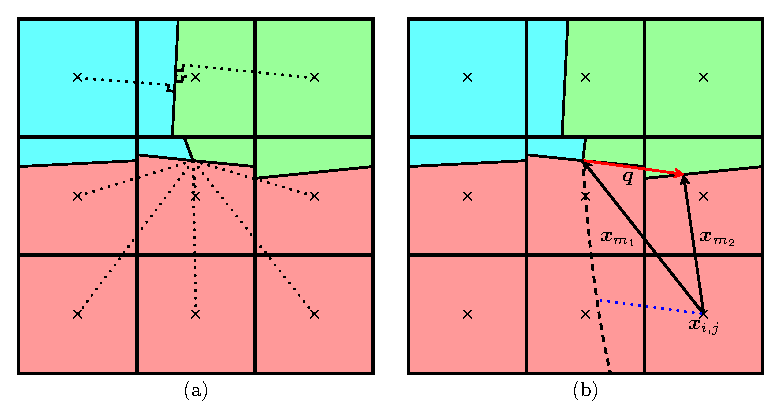
\includegraphics[width=0.8\textwidth]{redistancing_ils.eps}
%%  \scalebox{0.7}
%%  { %%Created by jPicEdt 1.4.1_03: mixed JPIC-XML/LaTeX format
%%Mon Aug 01 14:06:00 EDT 2016
%%Begin JPIC-XML
%<?xml version="1.0" standalone="yes"?>
%<jpic x-min="-0" x-max="126" y-min="-3" y-max="60" auto-bounding="true">
%<multicurve fill-color= "#ff9999"
%	 pstcustom= "opacity=0.5"
%	 fill-style= "solid"
%	 points= "(0,-0);(0,-0);(0,35);(0,35);(0,35);(20,36);
%	(20,36);(20,36);(20,37);(20,37);(20,37);(40,35);
%	(40,35);(40,35);(40,33);(40,33);(40,33);(60,35);
%	(60,35);(60,35);(60,0);(60,0);(60,0);(0,-0)"
%	 />
%<multicurve fill-color= "#99ff99"
%	 pstcustom= "opacity=0.5"
%	 fill-style= "solid"
%	 points= "(29.5,36);(29.5,36);(40,35);(40,35);(40,35);(40,33);
%	(40,33);(40,33);(60,35);(60,35);(60,35);(60,60);
%	(60,60);(60,60);(27,60);(27,60);(27,60);(26,40);
%	(26,40);(26,40);(29.5,36)"
%	 />
%<text text-vert-align= "center-v"
%	 anchor-point= "(30,-3)"
%	 fill-style= "none"
%	 text-frame= "noframe"
%	 text-hor-align= "center-h"
%	 >
%(a)
%</text>
%<multicurve fill-color= "#66ffff"
%	 pstcustom= "opacity=0.5"
%	 fill-style= "solid"
%	 points= "(0,35);(0,35);(20,36);(20,36);(20,36);(20,37);
%	(20,37);(20,37);(29.5,36);(29.5,36);(29.5,36);(28,40);
%	(28,40);(28,40);(26,40);(26,40);(26,40);(27,60);
%	(27,60);(27,60);(0,60);(0,60);(0,60);(0,35)"
%	 />
%<parallelogram p3= "(40,20)"
%	 p2= "(20,20)"
%	 p1= "(20,-0)"
%	 fill-style= "none"
%	 stroke-width= "0.4"
%	 />
%<parallelogram p3= "(20,20)"
%	 p2= "(0,20)"
%	 p1= "(0,-0)"
%	 fill-style= "none"
%	 stroke-width= "0.4"
%	 />
%<parallelogram p3= "(20,40)"
%	 p2= "(-0,40)"
%	 p1= "(0,20)"
%	 fill-style= "none"
%	 stroke-width= "0.4"
%	 />
%<parallelogram p3= "(40,40)"
%	 p2= "(20,40)"
%	 p1= "(20,20)"
%	 fill-style= "none"
%	 stroke-width= "0.4"
%	 />
%<multicurve stroke-style= "dotted"
%	 fill-style= "none"
%	 points= "(10,30);(10,30);(29.5,36);(29.5,36)"
%	 />
%<multicurve fill-style= "none"
%	 points= "(26.25,47.76);(26.25,47.76);(25.25,47.85);(25.25,47.85);(25.25,47.85);(25.34,48.85);
%	(25.34,48.85)"
%	 />
%<multicurve polydots-style= "polydots-plus"
%	 polydots-scale-v= "1"
%	 polydots-superimpose= "false"
%	 polydots-angle= "45"
%	 fill-style= "none"
%	 polydots-scale-h= "1"
%	 points= "(10,10);(10,10);(10,30);(10,30);(10,30);(10,50);
%	(10,50);(10,50);(30,50);(30,50);(30,50);(30,30);
%	(30,30);(30,30);(50,50);(50,50);(50.18,50.18);(50,30);
%	(50,30);(50,30);(50,10);(50,10);(50,10);(30,10);
%	(30,10)"
%	 polydots-size-minimum= "0.7"
%	 polydots-size-linewidth-scale= "3.5"
%	 />
%<parallelogram p3= "(60,40)"
%	 p2= "(40,40)"
%	 p1= "(40,20)"
%	 fill-style= "none"
%	 stroke-width= "0.4"
%	 />
%<parallelogram p3= "(60,20)"
%	 p2= "(40,20)"
%	 p1= "(40,-0)"
%	 fill-style= "none"
%	 stroke-width= "0.4"
%	 />
%<parallelogram p3= "(20,60)"
%	 p2= "(-0,60)"
%	 p1= "(0,40)"
%	 fill-style= "none"
%	 stroke-width= "0.4"
%	 />
%<parallelogram p3= "(40,60)"
%	 p2= "(20,60)"
%	 p1= "(20,40)"
%	 fill-style= "none"
%	 stroke-width= "0.4"
%	 />
%<parallelogram p3= "(60,60)"
%	 p2= "(40,60)"
%	 p1= "(40,40)"
%	 fill-style= "none"
%	 stroke-width= "0.4"
%	 />
%<multicurve stroke-style= "dotted"
%	 fill-style= "none"
%	 points= "(10,10);(10,10);(29.5,36);(29.5,36)"
%	 />
%<multicurve stroke-style= "dotted"
%	 fill-style= "none"
%	 points= "(30,10);(30,10);(29.5,36);(29.5,36)"
%	 />
%<multicurve stroke-style= "dotted"
%	 fill-style= "none"
%	 points= "(30,30);(30,30);(29.5,36);(29.5,36)"
%	 />
%<multicurve stroke-style= "dotted"
%	 fill-style= "none"
%	 points= "(50,30);(50,30);(29.5,36);(29.5,36)"
%	 />
%<multicurve stroke-style= "dotted"
%	 fill-style= "none"
%	 points= "(50,10);(50,10);(29.5,36);(29.5,36)"
%	 />
%<multicurve stroke-style= "dotted"
%	 fill-style= "none"
%	 points= "(10,50);(10,50);(26.5,48.75);(26.5,48.75)"
%	 />
%<multicurve stroke-style= "dotted"
%	 fill-style= "none"
%	 points= "(30,50);(30,50);(26.5,50.5);(26.5,50.5)"
%	 />
%<multicurve stroke-style= "dotted"
%	 fill-style= "none"
%	 points= "(50,50);(50,50);(26.49,52.36);(26.49,52.36)"
%	 />
%<multicurve fill-style= "none"
%	 points= "(27.75,50.32);(27.75,50.32);(27.63,49.32);(27.63,49.32);(27.63,49.32);(26.64,49.44);
%	(26.64,49.44)"
%	 />
%<multicurve fill-style= "none"
%	 points= "(27.86,52.2);(27.86,52.2);(27.75,51.2);(27.75,51.2);(27.75,51.2);(26.75,51.31);
%	(26.75,51.31)"
%	 />
%<multicurve fill-color= "#ff9999"
%	 pstcustom= "opacity=0.5"
%	 fill-style= "solid"
%	 points= "(66,-0);(66,-0);(66,35);(66,35);(66,35);(86,36);
%	(86,36);(86,36);(86,37);(86,37);(86,37);(106,35);
%	(106,35);(106,35);(106,33);(106,33);(106,33);(126,35);
%	(126,35);(126,35);(126,0);(126,0);(126,0);(66,-0)"
%	 />
%<multicurve fill-color= "#99ff99"
%	 pstcustom= "opacity=0.5"
%	 fill-style= "solid"
%	 points= "(95.5,36);(95.5,36);(106,35);(106,35);(106,35);(106,33);
%	(106,33);(106,33);(126,35);(126,35);(126,35);(126,60);
%	(126,60);(126,60);(93,60);(93,60);(93,60);(92,40);
%	(92,40);(92,40);(96,40);(96,40);(96,40);(95.5,36)"
%	 />
%<text text-vert-align= "center-v"
%	 anchor-point= "(96,-3)"
%	 fill-style= "none"
%	 text-frame= "noframe"
%	 text-hor-align= "center-h"
%	 >
%(b)
%</text>
%<multicurve fill-color= "#66ffff"
%	 pstcustom= "opacity=0.5"
%	 fill-style= "solid"
%	 points= "(66,35);(66,35);(86,36);(86,36);(86,36);(86,37);
%	(86,37);(86,37);(95.5,36);(95.5,36);(95.5,36);(96,40);
%	(96,40);(96,40);(92,40);(92,40);(92,40);(93,60);
%	(93,60);(93,60);(66,60);(66,60);(66,60);(66,35)"
%	 />
%<parallelogram p3= "(106,20)"
%	 p2= "(86,20)"
%	 p1= "(86,-0)"
%	 fill-style= "none"
%	 stroke-width= "0.4"
%	 />
%<parallelogram p3= "(86,20)"
%	 p2= "(66,20)"
%	 p1= "(66,-0)"
%	 fill-style= "none"
%	 stroke-width= "0.4"
%	 />
%<parallelogram p3= "(86,40)"
%	 p2= "(66,40)"
%	 p1= "(66,20)"
%	 fill-style= "none"
%	 stroke-width= "0.4"
%	 />
%<parallelogram p3= "(106,40)"
%	 p2= "(86,40)"
%	 p1= "(86,20)"
%	 fill-style= "none"
%	 stroke-width= "0.4"
%	 />
%<multicurve polydots-style= "polydots-plus"
%	 polydots-scale-v= "1"
%	 polydots-superimpose= "false"
%	 polydots-angle= "45"
%	 fill-style= "none"
%	 polydots-scale-h= "1"
%	 points= "(76,10);(76,10);(76,30);(76,30);(76,30);(76,50);
%	(76,50);(76,50);(96,50);(96,50);(96,50);(96,30);
%	(96,30);(96,30);(116,50);(116,50);(116.18,50.18);(116,30);
%	(116,30);(116,30);(116,10);(116,10);(116,10);(96,10);
%	(96,10)"
%	 polydots-size-minimum= "0.7"
%	 polydots-size-linewidth-scale= "3.5"
%	 />
%<parallelogram p3= "(126,40)"
%	 p2= "(106,40)"
%	 p1= "(106,20)"
%	 fill-style= "none"
%	 stroke-width= "0.4"
%	 />
%<parallelogram p3= "(126,20)"
%	 p2= "(106,20)"
%	 p1= "(106,-0)"
%	 fill-style= "none"
%	 stroke-width= "0.4"
%	 />
%<parallelogram p3= "(86,60)"
%	 p2= "(66,60)"
%	 p1= "(66,40)"
%	 fill-style= "none"
%	 stroke-width= "0.4"
%	 />
%<parallelogram p3= "(106,60)"
%	 p2= "(86,60)"
%	 p1= "(86,40)"
%	 fill-style= "none"
%	 stroke-width= "0.4"
%	 />
%<parallelogram p3= "(126,60)"
%	 p2= "(106,60)"
%	 p1= "(106,40)"
%	 fill-style= "none"
%	 stroke-width= "0.4"
%	 />
%<multicurve right-arrow= "head"
%	 fill-style= "none"
%	 points= "(116,10);(116,10);(95.5,36);(95.5,36)"
%	 />
%<multicurve right-arrow= "head"
%	 fill-style= "none"
%	 points= "(116,10);(116,10);(112.57,33.58);(112.57,33.58)"
%	 />
%<multicurve right-arrow= "head"
%	 fill-style= "none"
%	 points= "(95.64,36.01);(95.64,36.01);(112.64,33.68);(112.64,33.68)"
%	 stroke-color= "#ff0000"
%	 />
%<text text-vert-align= "top"
%	 anchor-point= "(116.08,8.99)"
%	 fill-style= "none"
%	 text-frame= "noframe"
%	 text-hor-align= "center-h"
%	 >
%$\bmx_{i,j}$
%</text>
%<text text-vert-align= "top"
%	 anchor-point= "(104.75,24)"
%	 fill-style= "none"
%	 text-frame= "noframe"
%	 text-hor-align= "right"
%	 >
%$\bmx_{m_1}$
%</text>
%<text text-vert-align= "top"
%	 anchor-point= "(115.25,24)"
%	 fill-style= "none"
%	 text-frame= "noframe"
%	 text-hor-align= "left"
%	 >
%$\bmx_{m_2}$
%</text>
%<text text-vert-align= "top"
%	 anchor-point= "(103.22,34.08)"
%	 fill-style= "none"
%	 text-frame= "noframe"
%	 text-hor-align= "center-h"
%	 >
%$\bmq$
%</text>
%<multicurve stroke-style= "dashed"
%	 stroke-dasharray= "1;1"
%	 fill-style= "none"
%	 points= "(95.5,36);(96.24,26.34);(97.24,12.89);(100.2,-0.07)"
%	 />
%<multicurve stroke-style= "dotted"
%	 fill-style= "none"
%	 points= "(98.45,12.36);(98.45,12.36);(115.66,10.05);(115.66,10.05)"
%	 stroke-color= "#0000ff"
%	 />
%</jpic>
%%End JPIC-XML
%PSTricks content-type (pstricks.sty package needed)
%Add \usepackage{pstricks} in the preamble of your LaTeX file
%You can rescale the whole picture (to 80% for instance) by using the command \def\JPicScale{0.8}
\ifx\JPicScale\undefined\def\JPicScale{1}\fi
\psset{unit=\JPicScale mm}
\psset{linewidth=0.3,dotsep=1,hatchwidth=0.3,hatchsep=1.5,shadowsize=1,dimen=middle}
\psset{dotsize=0.7 2.5,dotscale=1 1,fillcolor=black}
\psset{arrowsize=1 2,arrowlength=1,arrowinset=0.25,tbarsize=0.7 5,bracketlength=0.15,rbracketlength=0.15}
\begin{pspicture}(0,0)(126,60)
\newrgbcolor{userFillColour}{1 0.6 0.6}
\pspolygon[fillcolor=userFillColour,fillstyle=solid,opacity=0.5](0,-0)
(0,35)
(20,36)
(20,37)
(40,35)
(40,33)
(60,35)
(60,0)(0,-0)
\newrgbcolor{userFillColour}{0.6 1 0.6}
\pspolygon[fillcolor=userFillColour,fillstyle=solid,opacity=0.5](29.5,36)
(40,35)
(40,33)
(60,35)
(60,60)
(27,60)
(26,40)(29.5,36)
\rput(30,-3){(a)}
\newrgbcolor{userFillColour}{0.4 1 1}
\pspolygon[fillcolor=userFillColour,fillstyle=solid,opacity=0.5](0,35)
(20,36)
(20,37)
(29.5,36)
(28,40)
(26,40)
(27,60)
(0,60)(0,35)
\pspolygon[linewidth=0.4](20,-0)(20,20)(40,20)(40,0)
\pspolygon[linewidth=0.4](0,-0)(0,20)(20,20)(20,0)
\pspolygon[linewidth=0.4](0,20)(-0,40)(20,40)(20,20)
\pspolygon[linewidth=0.4](20,20)(20,40)(40,40)(40,20)
\psline[linestyle=dotted](10,30)(29.5,36)
\psline(26.25,47.76)
(25.25,47.85)(25.34,48.85)
\psdots[dotsize=0.7 3.5,dotstyle=+,dotangle=45](10,10)
(10,30)(10,50)(30,50)(30,30)(50,50)(50,30)(50,10)(30,10)
\pspolygon[linewidth=0.4](40,20)(40,40)(60,40)(60,20)
\pspolygon[linewidth=0.4](40,-0)(40,20)(60,20)(60,0)
\pspolygon[linewidth=0.4](0,40)(-0,60)(20,60)(20,40)
\pspolygon[linewidth=0.4](20,40)(20,60)(40,60)(40,40)
\pspolygon[linewidth=0.4](40,40)(40,60)(60,60)(60,40)
\psline[linestyle=dotted](10,10)(29.5,36)
\psline[linestyle=dotted](30,10)(29.5,36)
\psline[linestyle=dotted](30,30)(29.5,36)
\psline[linestyle=dotted](50,30)(29.5,36)
\psline[linestyle=dotted](50,10)(29.5,36)
\psline[linestyle=dotted](10,50)(26.5,48.75)
\psline[linestyle=dotted](30,50)(26.5,50.5)
\psline[linestyle=dotted](50,50)(26.49,52.36)
\psline(27.75,50.32)
(27.63,49.32)(26.64,49.44)
\psline(27.86,52.2)
(27.75,51.2)(26.75,51.31)
\newrgbcolor{userFillColour}{1 0.6 0.6}
\pspolygon[fillcolor=userFillColour,fillstyle=solid,opacity=0.5](66,-0)
(66,35)
(86,36)
(86,37)
(106,35)
(106,33)
(126,35)
(126,0)(66,-0)
\newrgbcolor{userFillColour}{0.6 1 0.6}
\pspolygon[fillcolor=userFillColour,fillstyle=solid,opacity=0.5](95.5,36)
(106,35)
(106,33)
(126,35)
(126,60)
(93,60)
(92,40)
(96,40)(95.5,36)
\rput(96,-3){(b)}
\newrgbcolor{userFillColour}{0.4 1 1}
\pspolygon[fillcolor=userFillColour,fillstyle=solid,opacity=0.5](66,35)
(86,36)
(86,37)
(95.5,36)
(96,40)
(92,40)
(93,60)
(66,60)(66,35)
\pspolygon[linewidth=0.4](86,-0)(86,20)(106,20)(106,0)
\pspolygon[linewidth=0.4](66,-0)(66,20)(86,20)(86,0)
\pspolygon[linewidth=0.4](66,20)(66,40)(86,40)(86,20)
\pspolygon[linewidth=0.4](86,20)(86,40)(106,40)(106,20)
\psdots[dotsize=0.7 3.5,dotstyle=+,dotangle=45](76,10)
(76,30)(76,50)(96,50)(96,30)(116,50)(116,30)(116,10)(96,10)
\pspolygon[linewidth=0.4](106,20)(106,40)(126,40)(126,20)
\pspolygon[linewidth=0.4](106,-0)(106,20)(126,20)(126,0)
\pspolygon[linewidth=0.4](66,40)(66,60)(86,60)(86,40)
\pspolygon[linewidth=0.4](86,40)(86,60)(106,60)(106,40)
\pspolygon[linewidth=0.4](106,40)(106,60)(126,60)(126,40)
\psline{->}(116,10)(95.5,36)
\psline{->}(116,10)(112.57,33.58)
\psline[linecolor=red]{->}(95.64,36.01)(112.64,33.68)
\rput[t](116.08,8.99){$\bmx_{i,j}$}
\rput[tr](104.75,24){$\bmx_{m_1}$}
\rput[tl](115.25,24){$\bmx_{m_2}$}
\rput[t](103.22,34.08){$\bmq$}
\psbezier[linestyle=dashed,dash=1 1](95.5,36)(96.24,26.34)(97.24,12.89)(100.2,-0.07)
\psline[linecolor=blue,linestyle=dotted](98.45,12.36)(115.66,10.05)
\end{pspicture}
 }
  \caption{Redistancing of the interface distance functions. (a) Measurements are shown for updating the interface distance function between the blue and green materials. The measurements for the cell in red material leads to a singular point for the interface distance function at the triple point. (b) Evaluation of extended interface distance function between the blue and green materials (dashed line) for the cell $\{i,j\}$. Dotted blue line shows the corresponding evaluated distance.}
  \label{fig:redistancing_ils}
\end{figure}

\section{Numerical tests and results}

\subsection{Zalesak problem}

In this section we report results for ``Zalesak's'' problem 
\cite{zalesak1979fully}.  We have previously reported the 
symmetric difference error for this test problem when using 
MOF reconstruction\cite{jemison2013coupled}.  
Here, we compare MOF to CMOF, and decision
tree machine learning to Gauss-Newton method for finding the
optimal slope.  

The problem setup for ``Zalesak's'' problem is as follows:
\begin{itemize}
	\item radius of notched disk=15 units.
	\item initial center of notched disk: (50,75)
	\item notch width: 5 units
	\item notch height: 25 units
	\item prescribed velocity: $u=-(\pi/314)(y-50)$,
		$v=(\pi/314)(x-50)$
\end{itemize}

In Table \ref{zalesaktable}, we report the symmetric difference
error (\ref{symmetricdiff}),
\begin{eqnarray}
	E_{sym}=
	|\Omega^{approx}\cap\Omega^{exact,complement}|+
	|\Omega^{approx,complement}\cap\Omega^{exact}|,
	\label{symmetricdiff}
\end{eqnarray}
after one full rotation of the notched disk (time is $628.0$
units).  Figure \ref{zalesak_compare} compares the MOF results to the
CMOF results on a $192^{2}$ grid.  For all Gauss-Newton
optimization results, we iterate until convergence with 
a tolerance of $10^{-10}$.  For the decision tree machine 
learning optimization results, we choose the best starting 
guess between the ``CLSVOF'' slope, ``decision tree slope,''
and the ``centroid slope.''  There are no iterations necessary
for the ``decision tree optimization'' results. 
In Table \ref{zalesakcost}, we report the cost of the 
Gauss-Newton optimization algorithm vs. the
``decision tree machine learning optimization.''

\begin{table}[h!]
\caption{Comparison of symmetric difference error:
	MOF versus CMOF and decision tree
	machine learning optimization (ML sample size equals
        $100^{2}$ or $50^{2}$) versus 
	Gauss Newton (GN)
	optimization ($t=628$) for Zalesak's problem.  }
\centering	
\begin{tabular}{|c|c|c|c|c|c|c|c|}
\hline
$\Delta x$ & $\Delta t$ & MOF & MOF & MOF & CMOF & CMOF & CMOF  \\ 
& & GN & ML $100^{2}$ & ML $50^{2}$ & GN & ML $100^{2}$ & ML $50^{2}$ 
\\ \hline 
$\frac{100}{96}$ & $\frac{628.0}{1155}$ & 6.8 & 8.1 & 9.6 & 19.0 & 18.9 & 18.9
\\ \hline
$\frac{100}{192}$ & $\frac{628.0}{2066}$ & 2.5 & 3.2 & 4.2 & 7.3 & 7.2 & 7.2 
\\ \hline
\end{tabular}  
\label{zalesaktable}	
\end{table}

\begin{table}[h!]
\caption{Comparison of reconstruction cost 
 (average number of iterations, reconstruction time): 
  MOF versus CMOF and decision tree
  machine learning optimization (ML, sample size 
  equals $100^{3}$) versus 
  Gauss Newton (GN)
  optimization ($t=628$) for Zalesak's problem.  }
 \centering
\begin{tabular}{|c|c|c|c|c|c|}
\hline
$\Delta x$ & $\Delta t$ & MOF-GN & MOF-ML & CMOF-GN & CMOF-ML   \\ \hline
$100/96$ & $628.0/1155$ & 3.5, 0.008 & 0, 0.007 & 7.5, 0.05 & 0, 0.02 \\ \hline
$100/192$ & $628.0/2066$ & 3.7, 0.019 & 0, 0.016 & 6.2, 0.09 & 0, 0.04 \\ \hline
\end{tabular}
\label{zalesakcost}
\end{table}

\begin{figure}[htbp]
\centering
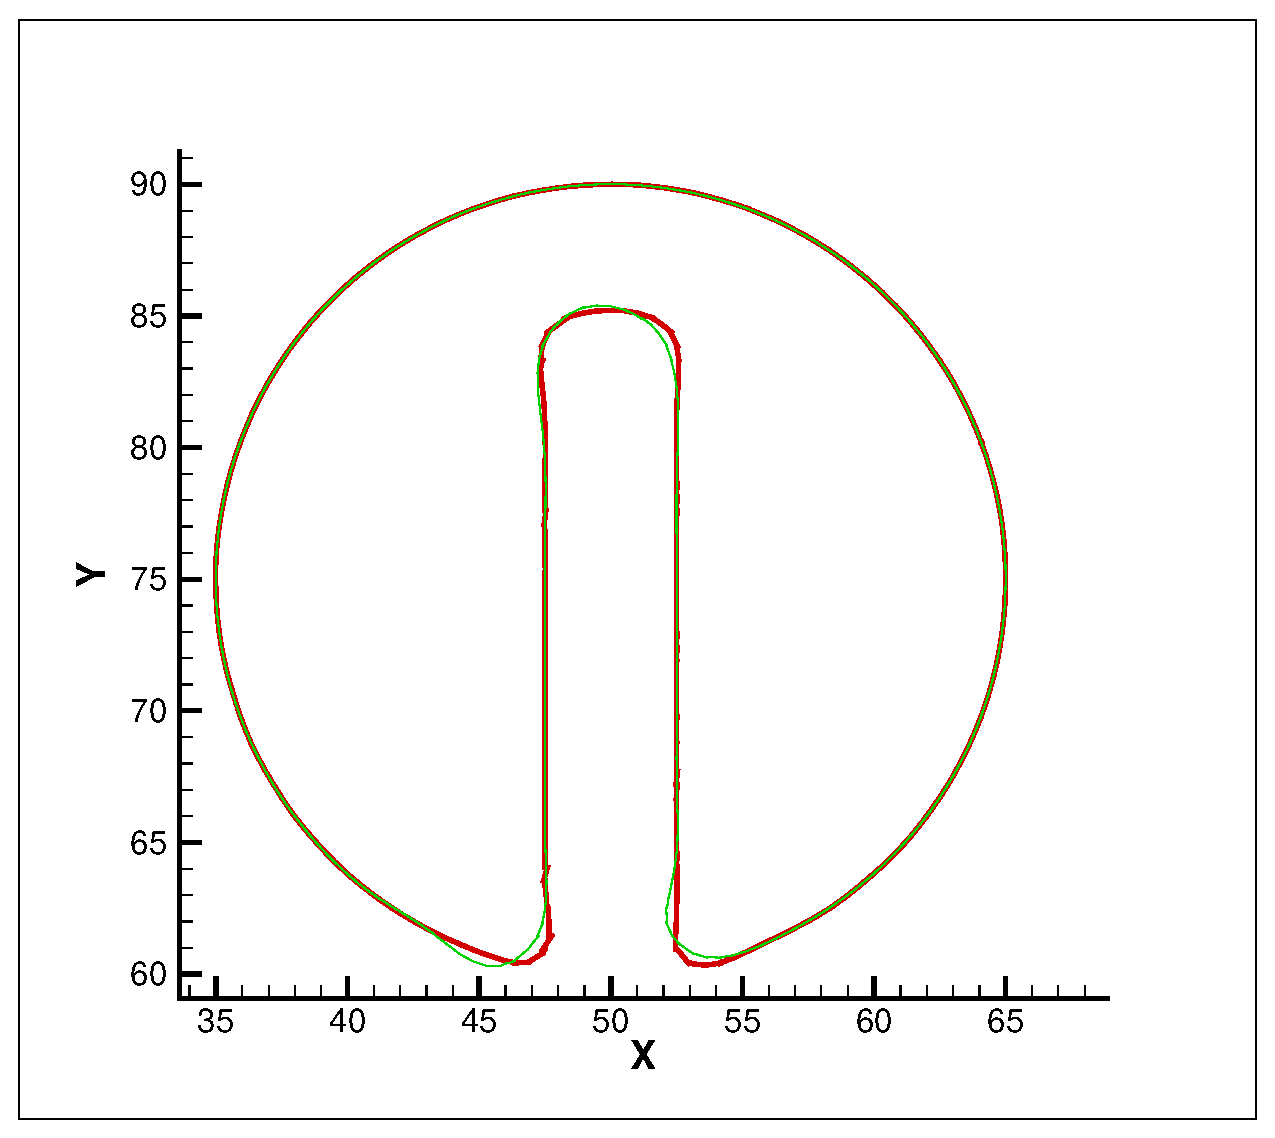
\includegraphics[width=0.8\textwidth]{zalesak_compare.eps}
\caption{Zalesak's problem at $t=628.0$.  
A comparison of MOF (red) with CMOF (green)
(using ``decision tree optimization'') on
a $192^{2}$ grid.  }
\label{zalesak_compare}
\end{figure}


\subsection{Bubble formation test problem; comparison of MOF with CMOF
  \label{bubform} }
%Figure 1E
%expected effective diameter: 0.499 cm
%nozzle radius 0.085cm
%multiply computed effective diameter by 0.085 
%We expect the run.out file to have 0.499/0.085=5.87

In this section we report results for the simulation of bubble formation
due to injection of gas through a nozzle at the bottom of the computational
domain.  The nozzle radius is $0.085$cm.
The effective fine grid resolution is $\Delta x^{fine}=0.010625$cm.

See Figure \ref{CMOF_bubble_formation} for the results using
the CMOF method and Figure \ref{MOF_bubble_formation} for the results using
MOF.  The results that we report correspond to the Figure 1E 
experiments reported
by \cite{helsby1955behaviour} and the simulations reported in 
\cite{OHTA20111059}.

The expected effective bubble diameter, after the initial transients end,
is $d_{effective}=0.499$cm.  We note in the results that there is 
unphysical noise and flotsam in the MOF
interface due to problems that start at the nozzle. The CMOF method does
not exhibit any noise.  

% 65.24 103.768  161.303
\begin{figure}[htbp]
\centering
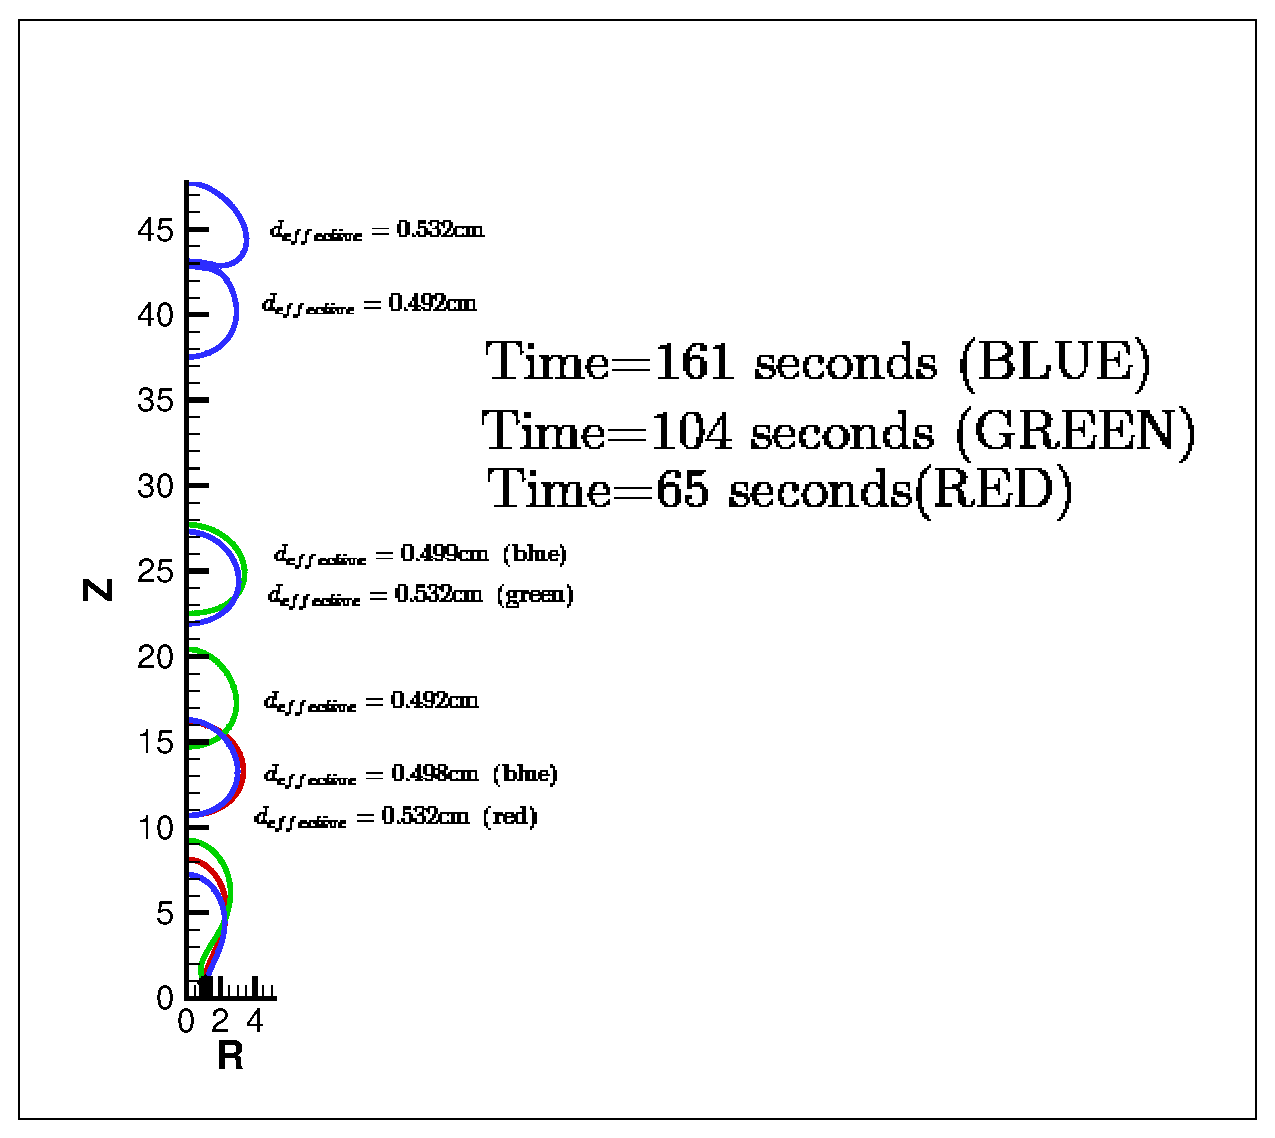
\includegraphics[width=0.9\textwidth]{CMOF_formation.eps} 
\caption{Computed results for the bubble formation problem using the
	CMOF method.  The step numbers are $13400$ ($t=65.2$), 
	$21600$ ($t=103.8$), and $34200$ ($t=161.3$).  The effective
	fine grid resolution is $\Delta x^{fine}=0.010625$cm}
 \label{CMOF_bubble_formation}
\end{figure}

\begin{figure}[htbp]
\centering
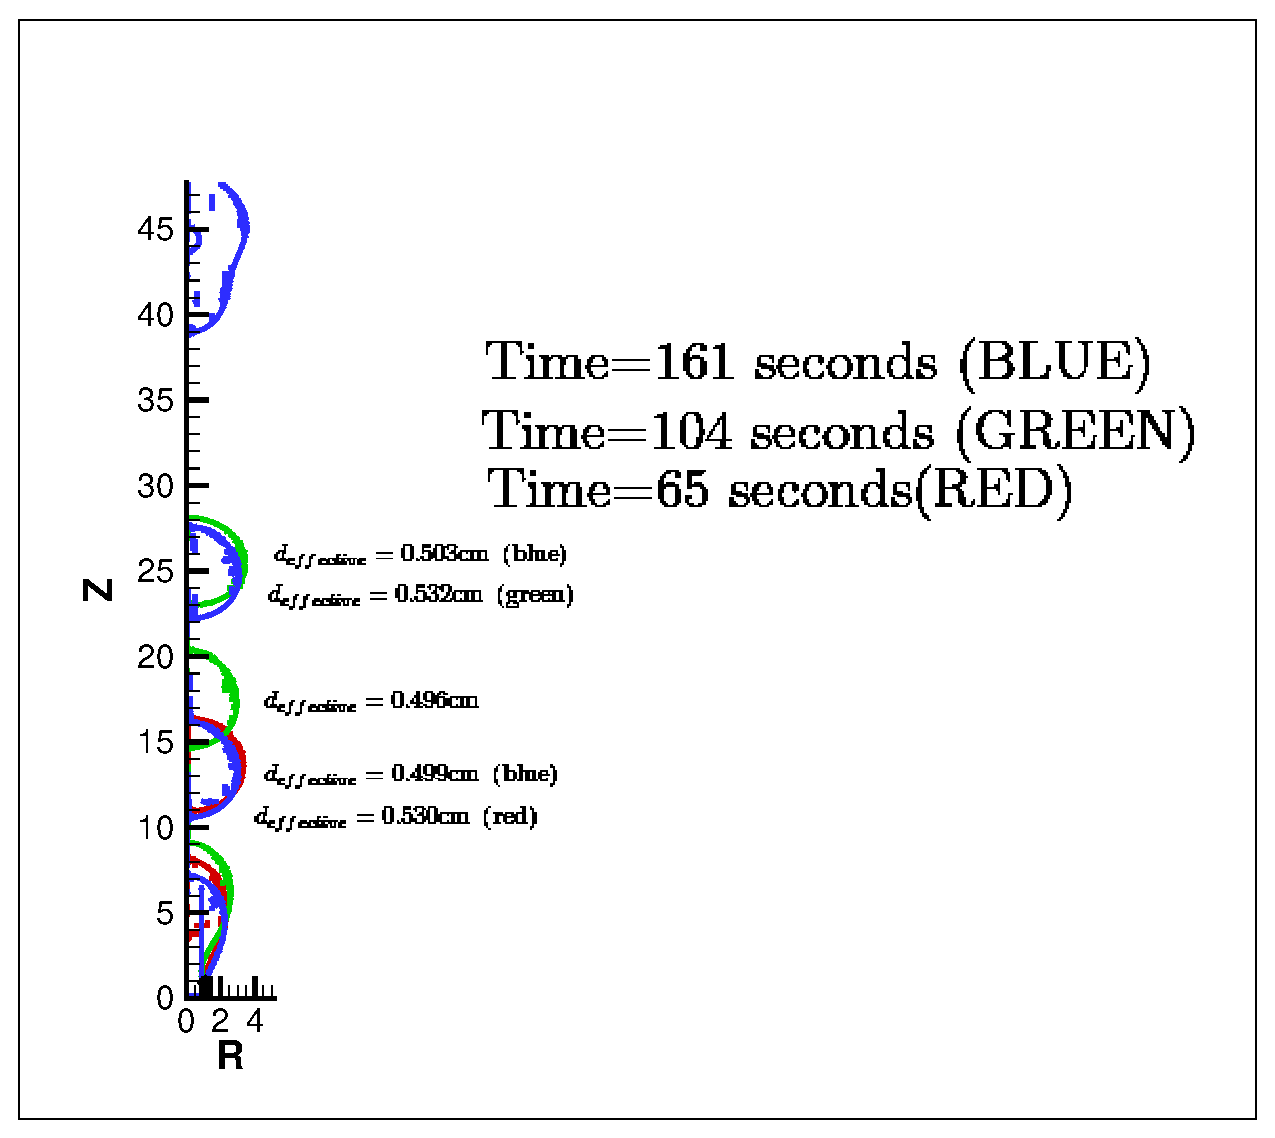
\includegraphics[width=0.9\textwidth]{MOF_formation.eps} 
\caption{Computed results for the bubble formation problem using the
	MOF method.  The step numbers are $13400$ ($t=64.9$), 
	$21600$ ($t=103.4$), and $34800$ ($t=161.1$).  The effective
	fine grid resolution is $\Delta x^{fine}=0.010625$cm}
 \label{MOF_bubble_formation}
\end{figure}


\subsection{Liquid lens test problem; comparison of MOF with CMOF 
\label{liqlens}}

In this section we report results for the simulation of the stretching
of a ``liquid lens'' due to surface tension forces at the junctions where
three materials meet.  We refer the reader to section 4.4 of 
\cite{kim2007phase} (phase field method) and
section 4.4 of \cite{li2015multiphase} (MOF method).  In contrast to our
previous simulations using the MOF method \cite{li2015multiphase} for the
Liquid Lens test, we intentionally add random noise to the initial
centroids.  Physically, due to the presence of surface tension and 
viscosity forces, the interface should become smooth, but the 
noise exhibited by the MOF results (see \ref{MOF_liquid_lens}) never 
disappear.  

The liquid lens test problem is setup as follows 
(see Figure \ref{liquid_lens}):
initially, there are three
materials with material 2 occupying a circle of diameter $0.3$ in 
the center of the domain, material
1 occupying the remaining top half of the computational domain, and 
material 3 occupying the
remaining bottom half of the computational domain. 
All three materials have the same unit density
and share the same viscosity of $\mu=1/60$. 
The surface tension coefficients between materials 1 and 2
and between materials 2 and 3 were set to $\sigma_{12}=2/45$ and
$\sigma_{23}=2/45$ respectively. The surface tension between materials
1 and 3 was set to $\sigma_{13}=5/90$.
Noise was artificially added to the centroids as follows,
\begin{eqnarray}
\bmx^{ref,noise}=\bmx^{ref}+(2r-1)\Delta x, \label{noise}
\end{eqnarray}
where $r$ is a random variable sampled from a uniform 
distribution, $0\le r\le 1$.
The expected steady-state solution has material 2 being stretched into
a lens shape with a major axis length of $L^{exact}_{0}=0.460$. 
We refer the reader to Figures \ref{CMOF_liquid_lens} (CMOF results), and
\ref{MOF_liquid_lens} (MOF results), and Table \ref{liquidlens_table}
(comparison between MOF and CMOF for this liquid lens test problem).
%%effective fine grid resolution: 128x128  1x1 domain.
%%(xcen-xcell)*=(2r-1)  0<=r<=1 
%%initial material 2 volume: 0.070682
%%MOF: .15 percent error
%%CMOF: 7E-8 percent error


\begin{table}[h!]
\caption{Comparison of MOF versus CMOF for the stretching of
	a liquid lens.  $L^{exact}_{0}$ is the expected steady
	state major axis length and $L_{0}$ is the computed
	steady state major axis length.
	Material 2 is the
	lens material, material 1 is above the lens, and
	material 3 is below the lens.  
        The initial centroids are randomly perturbed.  For the 
	MOF case, ``flotsam'' forms and migrates away from the
	``core'' interface and is then truncated.
}
 \centering
\begin{tabular}{|c|c|c|c|}
\hline
Method & $L_{0}$ & $L_{0}^{exact}$ & percent volume error $time=4.0$ \\ \hline
MOF    & 0.442  & 0.460 & $0.15$ percent   \\ \hline
CMOF   & 0.460  & 0.460 & $7.0e-8$ percent \\ \hline
\end{tabular}
\label{liquidlens_table}
\end{table}

See Figures 
\ref{CMOF_liquid_lens} and
\ref{MOF_liquid_lens}.

\begin{figure}[htbp]
\centering
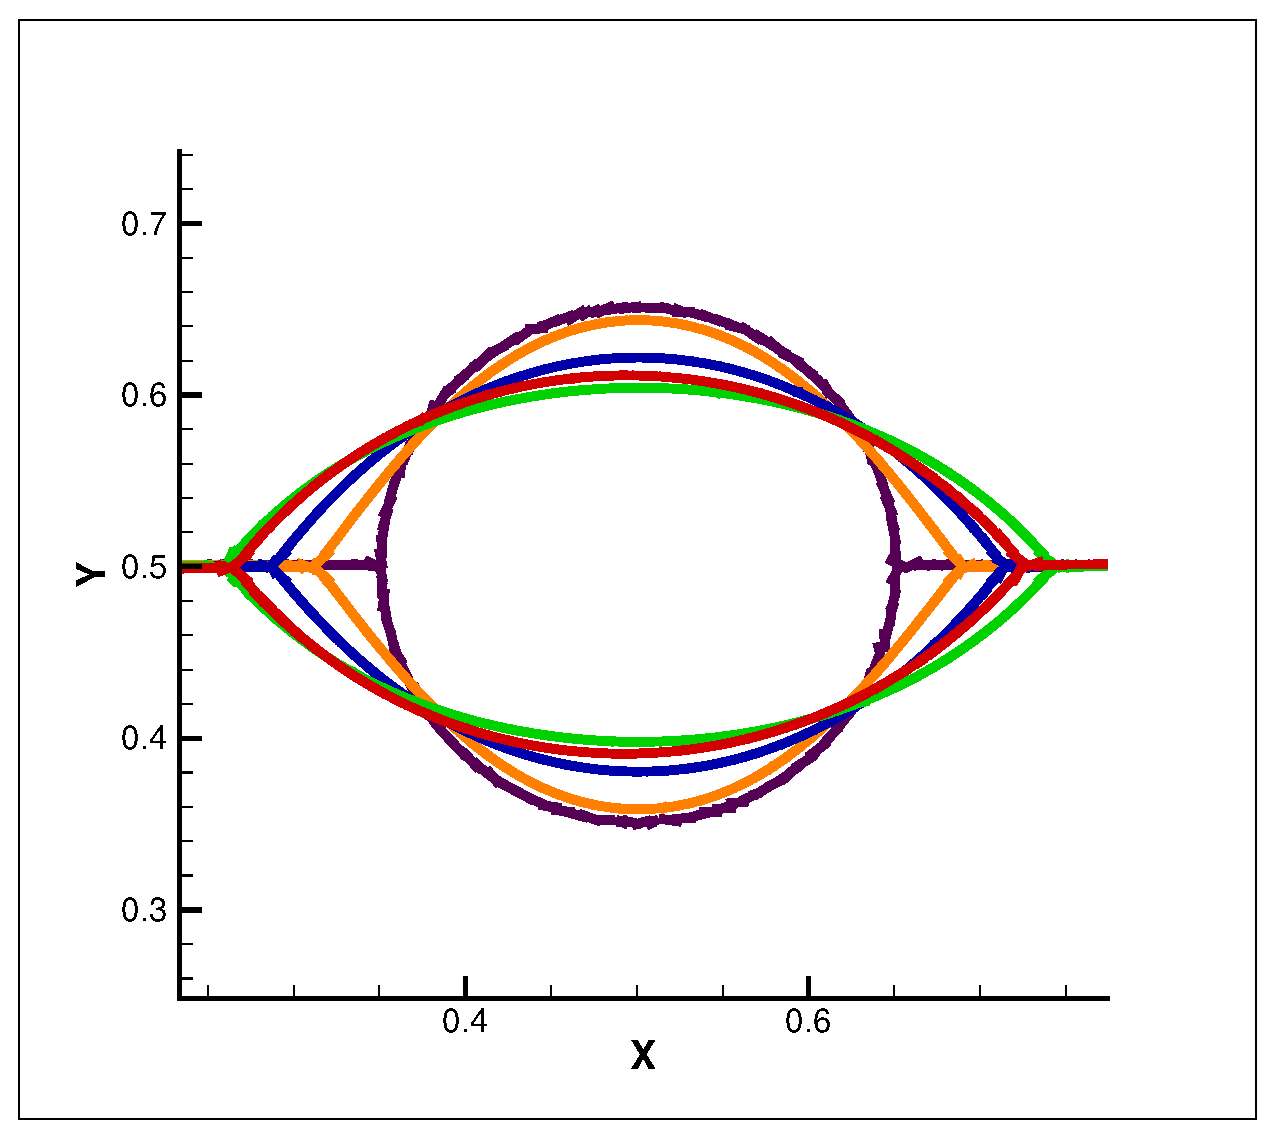
\includegraphics[width=0.8\textwidth]{CMOF_lens.eps} 
\caption{Stretching of a liquid lens computed using the CMOF method.  
	Times displayed are $0.0$ (brown), $0.187$ (orange), 
	$0.375$ (blue), $0.749$ (green), and $4.0$ (red).
	Material 2 is the
	lens material, material 1 is above the lens, and
	material 3 is below the lens.  
	The viscosity is the
	same for all 3 materials: $\mu=1/60$.  
	$\sigma_{12}=\sigma_{23}=2/45$.   $\sigma_{13}=5/90$.
        The computational domain dimensions are $1\times 1$ and
	the effective fine grid resolution is $128\times 128$.
	The initial centroids are randomly perturbed according
        to (\ref{noise}).  The CMOF method, by design, will 
        rapidly damp
        out the high frequency modes not recognizable by the
        curvature discretization algorithm.}
 \label{CMOF_liquid_lens}
\end{figure}

\begin{figure}[htbp]
\centering
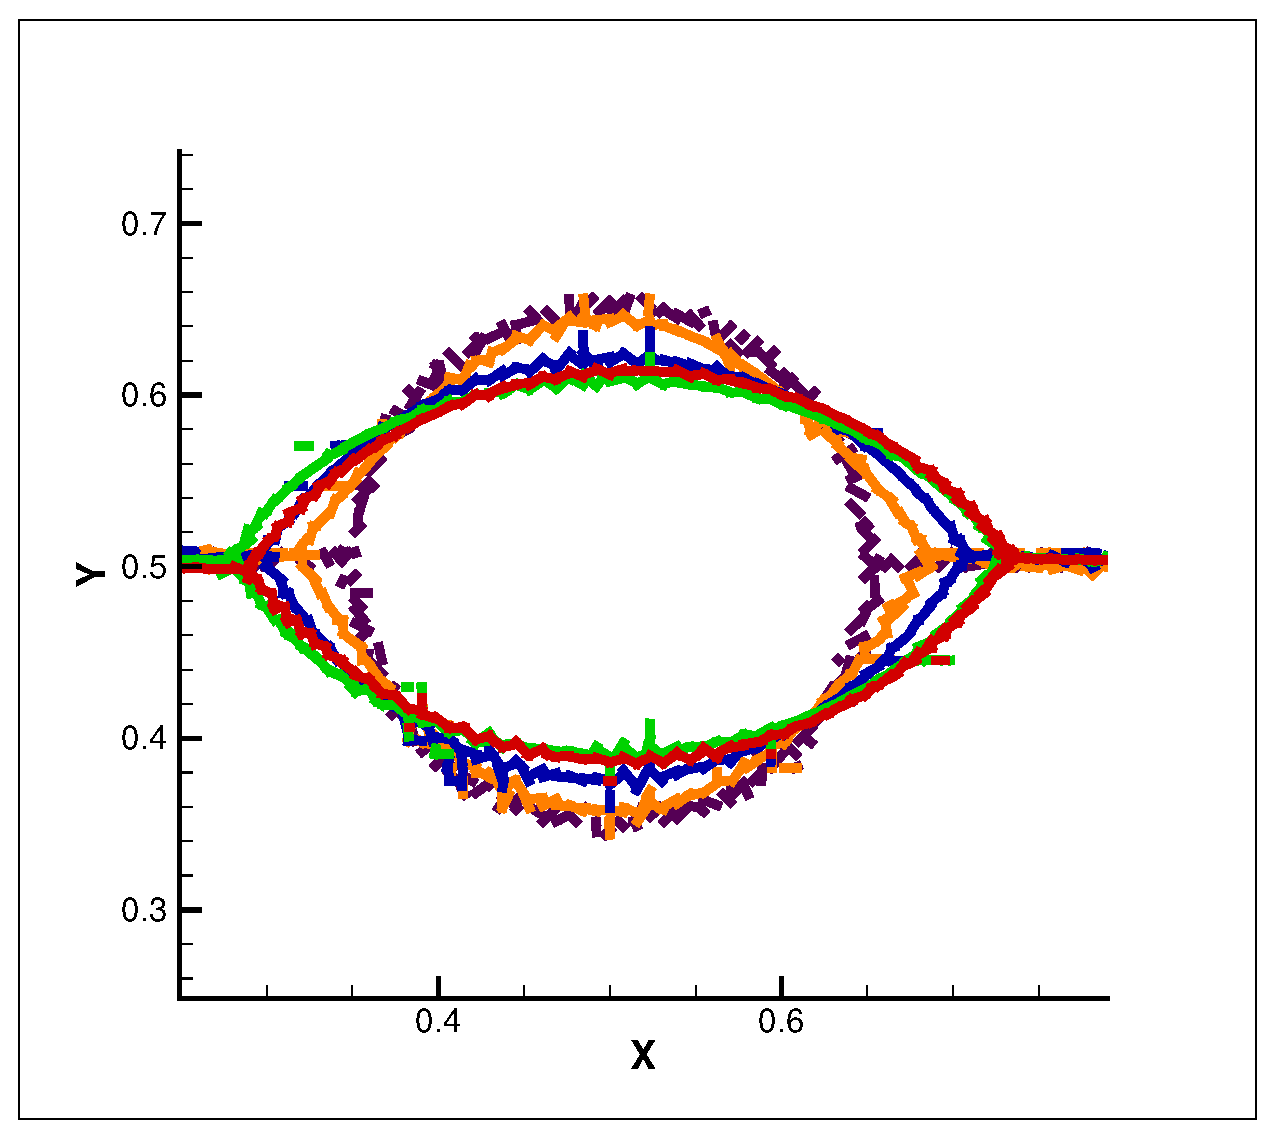
\includegraphics[width=0.8\textwidth]{MOFNOISE.eps} 
%(.290,.499) -> (.732,.505)  .442
\caption{Stretching of a liquid lens computed using the MOF method.  
	Times displayed are $0.0$ (brown), $0.187$ (orange), 
	$0.375$ (blue), $0.749$ (green), and $4.0$ (red).
	Material 2 is the
	lens material, material 1 is above the lens, and
	material 3 is below the lens.  
	The viscosity is the
	same for all 3 materials: $\mu=1/60$.  
	$\sigma_{12}=\sigma_{23}=2/45$.   $\sigma_{13}=5/90$.
        The computational domain dimensions are $1\times 1$ and
	the effective fine grid resolution is $128\times 128$.
	The initial centroids are randomly perturbed according
        to (\ref{noise}).  The MOF reconstruction method potentially
        generates ``high frequency'' signals unrecognized by
        conventional curvature discretization algorithms.
        }
 \label{MOF_liquid_lens}
\end{figure}


\subsection{Freezing of a water droplet on a cold substrate; comparison with
  experiments and convergence study. \label{freezing_sec} }

In this section we test our CMOF algorithm for simulating the freezing
of a water droplet on a cold substrate.  We refer the reader to 
Figure \ref{ice_levelset} which illustrates the initial conditions for
our test.  The temperature in the cold substrate is prescribed to be
$T_{w}$.  We shall compare our results with
that which is reported in \cite{hu2010icing}.  
In Tables \ref{paramtable} and \ref{paramtable_int},
we report the physical properties, in CGS units,
used in our simulations.

\begin{table}[h!]
\caption{Physical properties of air, water, ice, and substrate for comparing 
	with the icing experiments from \cite{hu2010icing}.  
}
 \centering
\begin{tabular}{|c|c|c|c|c|}
\hline
variable             & substrate & ice       & water     & air\\ \hline
density ($\rho$)     & rigid     & $0.917$   & $1.0$     & $0.00129$ \\ \hline
viscosity ($\mu$)    & rigid     & rigid     & $1.7e-2$  & $1.7e-4$ \\ \hline
spec. heat ($C_{p}$) & $T=T_{w}$ & $2.03e+7$ & $4.21e+7$ & $1.0e+7$ \\ \hline
thermal cond. ($k$)  & $T=T_{w}$ & $2.2e+5$  & $0.55e+5$ & $0.026e+5$ \\ \hline
initial temp.        & $T_{w}$   & $T_{w}$   & $273.0$   & $293.0$ \\ \hline
\end{tabular}
\label{paramtable}
\end{table}

\begin{table}[h!]
\caption{Interfacial Physical properties for comparing 
	with the icing experiments from \cite{hu2010icing}.  
}
\centering
\begin{tabular}{|c|c|}
\hline
variable                                & value \\ \hline
surface tension ($\gamma$)              & $72.8$ \\ \hline
%%SUSSMAN REVISION
%%added mass ($\rho_{\mbox{added mass}}$) & $1.0e+6$ \\ \hline
%%added mass ($\rho_{\mbox{added mass}}$) & $1.0e+9$ \\ \hline
physical latent heat ($L$) & $3.34e+9$ \\ \hline
modeling latent heat ($L_{\mbox{model}}$) & $65.0e+9$ \\ \hline
saturation temperature ($T_{sat}$) & $273.0$ \\ \hline
\end{tabular}
\label{paramtable_int}
\end{table}

Remarks:
\begin{itemize}
\item In our icing simulations we intentionally add mass to the
interface; we refer to sub-section 
\ref{addmass_sec} 
%%put the incremental gravity pressure formulation in addmass_sec
%%p^incremental=p-rho gvec dot (x y z)
%%rho=rhoL H + rhoG (1-H)=rhoG + (rhoL-rhoG)H
%%grad p^{inc}=grad p-grad(rho g z)=
%%grad p-\gvec\dot(x y z) grad rho - rho gvec =
%%grad p - \gvec\dot(x y z) (rhoL-rhoG)grad H - rho gvec
%%grad p=grad p^{inc} +
%%   \gvec\dot(x y z) (rhoL-rhoG)grad H + rho gvec
%%-grad p/rho + gvec=
%% -grad p^{inc}/rho -
%%   \gvec\dot(x y z) (rhoL-rhoG)grad H/rho 
below for
details of our added mass model.  The surface tension time step
constraint (\ref{stiffconstraint}),
\begin{eqnarray*}
\Delta t< \Delta x^{3/2}
    \sqrt{\frac{\rho_{L}+\rho_{G}}
          {2\pi\sigma}},
\end{eqnarray*}
is greatly relaxed by adding mass to the interface,
\begin{eqnarray}
\Delta t< \Delta x^{3/2}
    \sqrt{\frac{\rho_{\mbox{added mass}}}
          {\pi\sigma}}.
	  \label{reduced}
\end{eqnarray}
We have heuristically chosen
$\rho_{\mbox{added mass}}=1.0e+6$ for simulations with $L=3.34e+9$ and
$\rho_{\mbox{added mass}}=1.0e+9$ for simulations with $L=65.0e+9$.
The criteria that we use in our choice of
$\rho_{\mbox{added mass}}$ is that the 
surface tension time step constraint 
(\ref{reduced}) is maximally relaxed while the
modified ``numerical'' characteristic surface tension wave speed,
\begin{eqnarray*}
\sqrt{\frac{\pi\sigma_{m1,m2}}{\Delta x \rho_{\mbox{added mass}}}}
\end{eqnarray*} 
is still maintained to be
much faster than the characteristic speed associated with 
freezing (\ref{uphasechange}).
Similar strategies were
taken in the simulation results reported by
\cite{shetabivash2020multiple,vu2015numerical,vahab2016adaptive}.
\item In Table \ref{freezing_time}, we plot the time to freeze 
 the droplet as a function of the wall temperature and using
 the physical value for latent heat.  These results are 
 consistent with the Stefan model (see Figures \ref{rect_freeze}
 and \ref{freezing_verification}) but predict a freezing
 rate much faster than that which appears in the 
 experiments \cite{hu2010icing}.  In order to get agreement
 with experiments we artificially increased the
 latent heat (see $L_{\mbox{model}}$ in 
 Table \ref{paramtable_int}) which then 
 enabled us to get much closer agreement with experiments 
 for all of the wall temperature cases.  See
 Table \ref{freezing_time}.
\item The ``triple point'' model for capillary forces is different from
 our previous research reported in \cite{vahab2016adaptive}.  Previously, we
 had prescribed an artificial ``mushy zone'' layer at the
 ice-water interface in which the ice was allowed to deform 
 like a fluid.  Also, previously, we had prescribed
 artificial surface tension 
 coefficients for the 
 ice-air and ice-water interfaces in order to enforce a static
 triple point contact angle condition.  
 In the present work, we model the
 ice as a rigid solid, with the only exception 
 that the ice-water interface
 is allowed to propagate due to phase change.  The surface tension
 force at the triple point depends only on the water/gas surface
 tension coefficient.  See Figure \ref{ice_levelset}. Also, we
 refer the reader to the following article \cite{lyu2021hybrid}.
\end{itemize}

In order to verify that our numerical method is consistent with the
``Stefan'' freezing model, we compared our simulation results
for the freezing of a 
planar interface in the axisymmetric 3D $R-Z$ coordinate system,
with the results of the corresponding 1D Stefan problem in which
a known ``analytic'' solution exists (see (\ref{1dsoln}) and
\cite{welch2000volume}):
\begin{eqnarray}
\lambda e^{\lambda^{2}}\mbox{erf}(\lambda)=
\frac{cp(\theta_{wall}-\theta_{sat})}{h_{lg}\sqrt{\pi}} \label{1dsoln} \\
x(t)=2\lambda\sqrt{\alpha t} \hspace{15pt} \alpha=\frac{k}{\rho L} 
\nonumber 
\end{eqnarray}
In this test, the
density ratio was set to one and the substrate temperature was prescribed
as $-6$ degrees Celsius.  The latent heat was set to the physical
value of $3.34e+9$ ergs per gram.  Figure \ref{rect_freeze} shows
our simulation results for this test problem and 
Figure \ref{freezing_verification}
shows a comparison of the position of the water/ice front versus time
between simulation (the curve labeled ``Cylindrical\_ice'') and 
1D analytical results (the curve labeled ``1D\_ice'').  The grid used in our
simulation was $64\times 64$ grid cells. The maximum relative
error between simulation and analytical solution is $1.1$ percent.
% 58 -> 234 pixels = 176 pixels   8 pixels (2 pixels)

The next test that we did was to check for convergence under grid 
refinement.  In Figure \ref{freezing_conv_study} we compare the
position of the water-ice interface (at $r=0$) for 
three different grid resolutions: $32^{2}$, $64^{2}$, and $128^{2}$.
For this test we used the physical value for Latent heat, $L=3.34e+9$,
and the substrate temperature was maintained at $-6$ degrees Celsius.
In Figure \ref{freezing_frames}, we display the interface(s) and 
temperature contours for the finest grid case, $128^{2}$.  We note that the 
interface shape is as expected in that the water/air interface is smooth
prior to the end stage of the liquid drop freezing process.
The last frame 
shows the classical ``tip'' due to expansion of the ice. 

Finally, in Table \ref{freezing_time} we report on the time
to completely freeze a water droplet as a 
function of the wall temperature (degrees Celsius)
and Latent heat.  We compare our simulation Results with
experiments from \cite{hu2010icing}.  
We note that when the physical latent heat was used, 
$3.34e+9$,
the freezing times were much too fast.  Since we get good agreement
with the comparable 1D Stefan model, 
(see Figure \ref{freezing_verification}, ``Hemispherical ice'' vs
``1D ice''), we hypothesize that the discrepancy is due to incorrect
modeling rather than a problem with our algorithm.  Using our 1D
model as a guide, we determined that increasing the latent heat
to be $65.0e+9$ enabled us to have agreement for a wide range of
prescribed substrate temperatures.


\subsubsection{Added Mass model for static freezing test problem 
\label{addmass_sec} }

Our added mass model relies on the momentum equation being 
discretized in incremental gravity - pressure form.  We replace
(\ref{pressuregrad}) with
\begin{eqnarray}
\lefteqn{ \frac{\bmu^{n+1}-\bmu^{\ast}}{\Delta t}=
 -\frac{\nabla p^{\mbox{incremental},n+1}}{\rho^{\mbox{MAC,mix},n+1}}- }
\nonumber   \\
& & \sum_{m_{1}<m_{2}} \bmg\cdot\bmx
\frac{(\rho_{m_{1}}-\rho_{m_{2}})\nabla H(\phi_{m_{1}})}
     {\rho^{\mbox{MAC,mix},n+1}}-
\frac{\sum_{m=1}^{M} \gamma_{m}\kappa_{m}\nabla H(\phi_{m})}
	{\rho^{\mbox{MAC,mix},n+1}} 
\label{pressuregrad_increment}
\end{eqnarray}
where 
\begin{eqnarray*}
p=p^{\mbox{incremental}}+\rho \bmg \cdot\bmx 
\end{eqnarray*}
The cell-centered
mixture of the density, $\rho^{\mbox{mix}}$, 
as it appears 
in the viscosity 
equation (\ref{diffusion3}), is determined from volume weights in a 
given cell $(i,j)$.  The
volume weights are derived from the CMOF
reconstructed interface (see \cite{pei2019hierarchical} or
Figure \ref{dencell_mixture}).
If the level set
function changes sign for an appropriate pair of materials, the
user defined ``added mass density,'' 
$\rho_{\mbox{added mass}}$,
is used in place of the
volume averaged density.  The level set function values in all
cells in the given 9 point stencil (27 points in 3D)
are tested.  Also, if the 
volumes for the appropriate materials are positive in the
center cell, $(i,j)$, then we replace the given density
with the ``added mass density.''

The ``MAC'' grid 
mixture of the density, $\rho^{\mbox{MAC,mix}}$, 
as it appears 
in the incremental pressure gradient 
equation (\ref{pressuregrad_increment}), 
is determined from volume weights in a 
given MAC grid control volume $(i+1/2,j)$.  The
volume weights are derived from the CMOF
reconstructed interface 
(see \cite{pei2019hierarchical,VAHAB2021} or 
Figure \ref{denMAC_mixture}). 
If the level set
function changes sign for the appropriate materials, a 
user defined ``added mass density,'' 
$\rho_{\mbox{added mass}}$,
is used in place of the
volume averaged density.  The level set function values in 
cells $(i,j)$ and $(i+1,j)$ (for the $(i+1/2,j)$ face)
are tested.  Also, if the 
``face'' volumes for the appropriate 
materials are positive in the MAC grid 
control volume, $(i+1/2,j)$,
then we replace the given density
with the ``added mass density.''

% k= 2 pi/dx
% ucap=sqrt(2 pi/dx) sqrt(sigma/(rho1+rho2))
% ucap dt <dx
% dt<dx/ucap=dx^(3/2)sqrt((rho1+rho2)/(2 pi sigma))
%
\begin{figure}[htbp] 
  \centering
    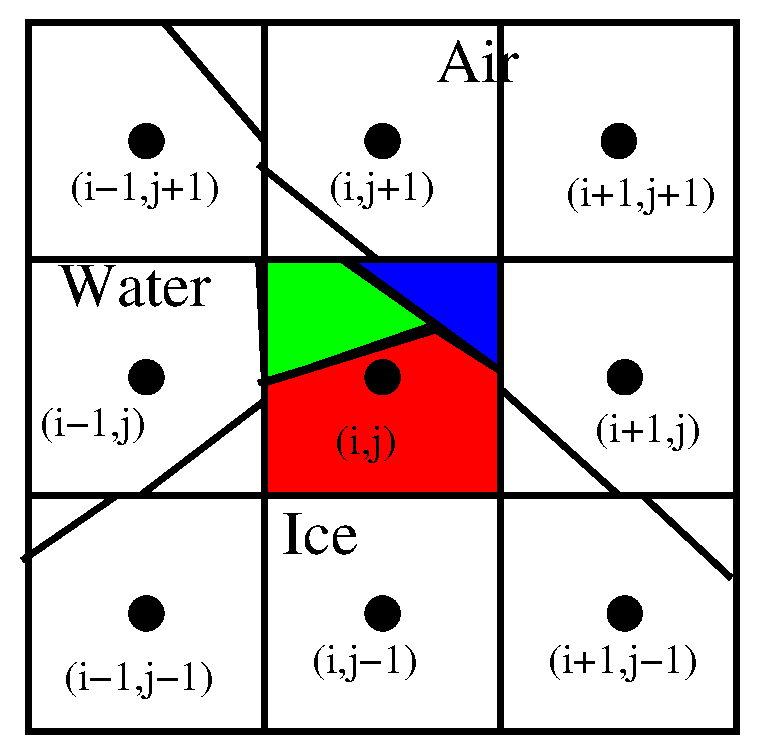
\includegraphics[width=0.7\textwidth]{dencell_mixture.eps}
  \caption{
   An illustration of the derivation of the volume weights for
   computing the cell centered
   mixture product of density and specific
   heat $\rho C_{p}$, and also for computing the volume weights for
   computing the cell centered
   mixture density $\rho$ as it appears in the 
   viscosity equation.  In the latter case, 
   if the level set
   function changes sign for the appropriate materials, a 
   user defined ``added mass density'' is used in place of the
   volume averaged density.  The level set function values in all
   cells in the given 9 point stencil (27 points in 3D)
   are tested.  Also, if the 
   volumes for the appropriate materials are positive in the
   center cell, $(i,j)$, then we replace the given density
   with the ``added mass density.''
   }
  \label{dencell_mixture} 
\end{figure}


\begin{figure}[htbp] 
  \centering
    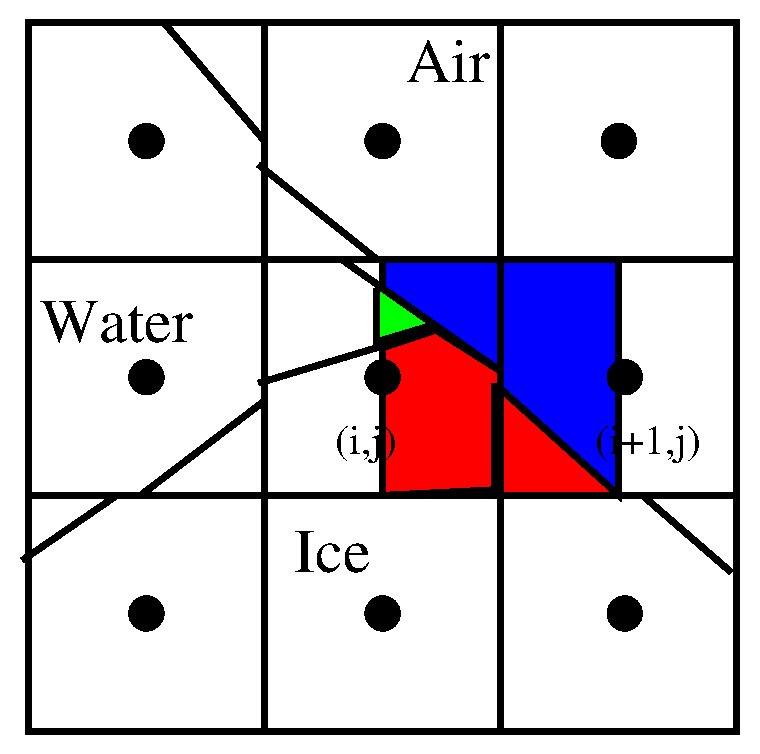
\includegraphics[width=0.7\textwidth]{denMAC_mixture.eps}
  \caption{
   An illustration of the derivation of the volume weights for
   computing the 
   ``MAC'' grid 
   mixture of the density, $\rho^{\mbox{MAC,mix}}$, 
   as it appears 
   in the pressure gradient 
   equation (\ref{pressuregrad}).
   $\rho^{\mbox{MAC,mix}}$ 
   is determined from volume weights in a 
   given MAC grid control volume $(i+1/2,j)$.  The
   volume weights are derived from the CMOF
   reconstructed interface.
   If the level set
   function changes sign for the appropriate materials, a 
   user defined ``added mass density'' is used in place of the
   volume averaged density.  The level set function values in 
   cells $(i,j)$ and $(i+1,j)$ (for the $(i+1/2,j)$ face)
   are tested.  Also, if the 
   ``face'' volumes for the appropriate 
   materials are positive in the MAC grid 
   control volume, $(i+1/2,j)$,
   then we replace the given density
   with the ``added mass density.''
   }
  \label{denMAC_mixture} 
\end{figure}


\begin{table}[h!]
	\caption{Time to freeze a water droplet with 
	initial volume $4.95e-5\mbox{cm}^{3}$ as a 
	function of the wall temperature (degrees Celsius)
	and Latent heat.  Results are
	compared with experiments from \cite{hu2010icing}.  
	Much closer agreement is made with experiments when
	the latent heat is prescribed as $65.0e+9$ as opposed
	to when he latent heat is the physical value
	$3.34e+9$.
}
% -6, fine, 0.579
% -6, med, 0.590
\centering
\begin{tabular}{|c|c|c|c|}
\hline
Wall temperature & Latent heat & time (computed) & time (exp) 
	 \\ \hline
$-2.0$ & $3.34e+9$ & $2.0$ & $32.5$ \\ \hline
$-3.0$ & $3.34e+9$ & $1.2$ & $21.0$ \\ \hline
$-4.0$ & $3.34e+9$ & $0.9$ & $16.0$ \\ \hline
$-5.0$ & $3.34e+9$ & $0.7$ & $13.5$ \\ \hline
$-2.0$ & $65.0e+9$ & $35.7$ & $32.5$ \\ \hline
$-3.0$ & $65.0e+9$ & $22.6$ & $21.0$ \\ \hline
$-4.0$ & $65.0e+9$ & $16.7$ & $16.0$ \\ \hline
$-5.0$ & $64.0e+9$ & $13.0$ & $13.5$ \\ \hline
\end{tabular}
\label{freezing_time}
\end{table}


\begin{figure}[htbp]
\centering
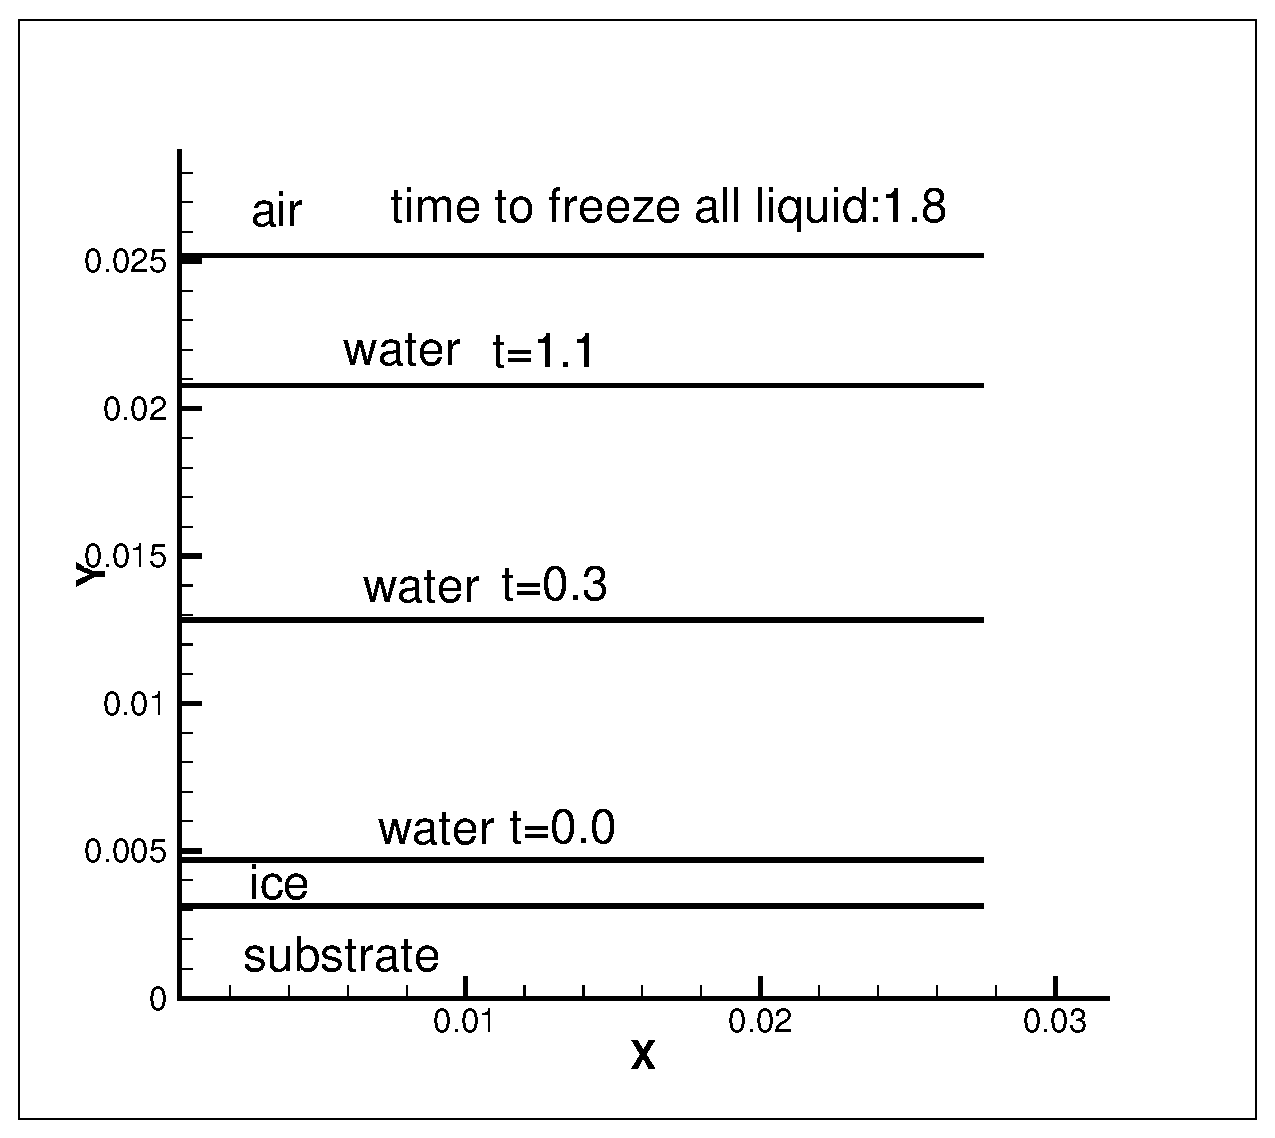
\includegraphics[width=0.8\textwidth]{freeze1d.eps} 
\caption{Freezing of a planar interface in R-Z coordinates.  
 The substrate temperature
 is maintained at $-2$ degrees Celsius. 
 The Latent Heat is $3.34e+9$ ergs per gram and
 the grid size is $64\times 64$. }
\label{rect_freeze}
\end{figure}


\begin{figure}[htbp]
\centering
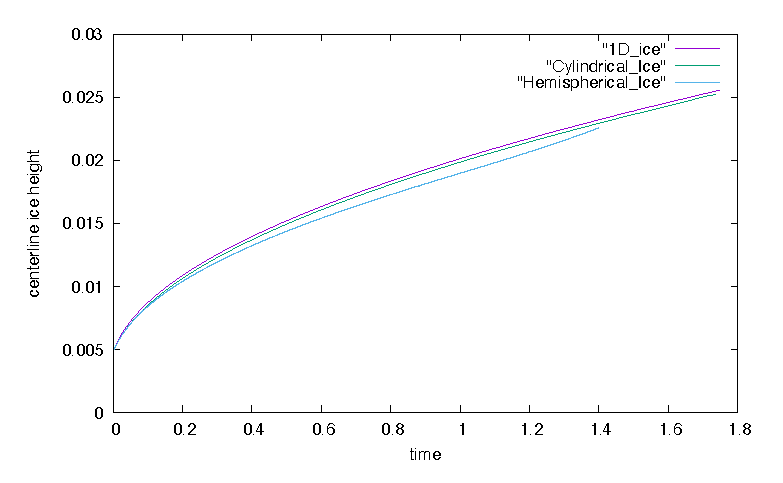
\includegraphics[width=0.8\textwidth]{freezing_verification.eps}
\caption{Verification of the Stefan model for freezing.
  The rate of freezing of a Hemispherical droplet is within 
  $5$ percent of the ``comparable'' cylindrical droplet freezing case.
  The Cylindrical freezing rate agrees within $1.1$ percent of the
  1D analytical model.}
 \label{freezing_verification}
\end{figure}


\begin{figure}[htbp]
\centering
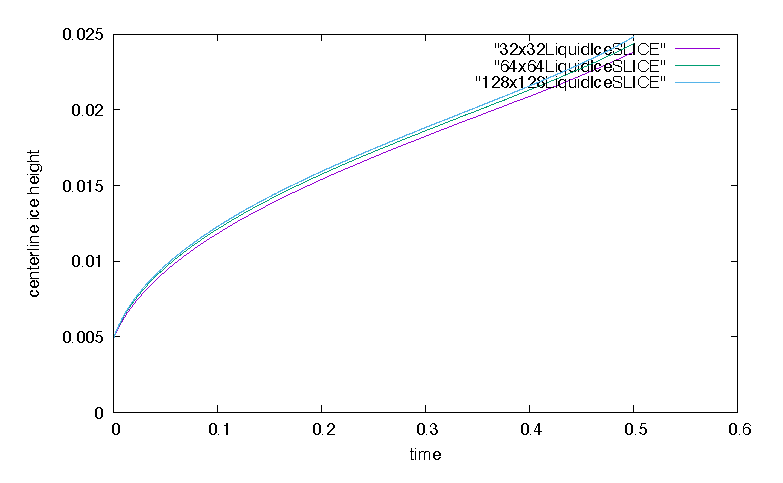
\includegraphics[width=0.8\textwidth]{ICE_HEIGHT.eps}
\caption{Convergence study for the solidification of a liquid drop
 on a cold substrate.  The position of the liquid-ice interface is
 plotted versus time.
 The substrate temperature is maintained at $-6$ degrees Celsius. 
 The Latent Heat is $3.34e+9$ ergs per gram and
 the grid sizes are 
 $32\times 32$,
 $64\times 64$, and
 $128\times 128$. }
 \label{freezing_conv_study}
\end{figure}


%(cite Aanjanaya, Denner, etc)
%\cite{JARAUTA20181196}
%\cite{IDelsohnDelPinRossiOnate2009}
%\cite{hu2010icing}
%initial ice thickness: icethick(0)=.003125 cm
%substrate z=0.0015625 cm
%height of water over the ice: 0.0205 cm
%(coordinate of initial water peak:z=0.0252cm)
%initial water base radius for contact region with ice: r0=0.0372cm
%average water base radius assuming icethick'(t)=constant: 0.0275cm
%initial liquid volume: $4.95e-5 cm^{3}$
%initial ice volume: $7.02e-6 cm^{3}$


\begin{figure}[htbp]
\centering
\includegraphics[width=0.4\textwidth]{freezing0000May2023.eps} 
\includegraphics[width=0.4\textwidth]{freezing3200May2023.eps}  \\
\includegraphics[width=0.4\textwidth]{freezing5200May2023.eps}  
\includegraphics[width=0.4\textwidth]{freezing6800May2023.eps}  
\caption{
 4 snapshots of the liquid, gas, ice interfaces over time: left to right,
 top to bottom: $t=0$, $t=0.27$, $t=0.44$, and $t=0.59$.
 The substrate temperature is maintained at $-6$ degrees Celsius. 
 The Latent Heat is $3.34e+9$ ergs per gram and
 the grid size is $128\times 128$.
}
\label{freezing_frames}
\end{figure}


\subsection{Comparison of simulations with experiments for the
  break-up of a gas bubble due to a liquid jet in microgravity.
  \label{TPCEsec} }

%zero-gravity
%3D axisymmtric results for the simulation of bubble dynamics in 
%the ZBOT (Kassemi, Kartuzova, and Hylton 2018) tank 
%using the HFE7000 material, 
%but with inflow conditions 
%corresponding to the
%microgravity experiments reported by Bentz, Meserole, and Knoll (1992).  

There were a number of experiments performed in microgravity
(see \cite{bentz1992jet} and \cite{bentz1993low})
in which a liquid jet was created in an experimental tank and the
jet impinged upon a spherical gas bubble in the upper part of the
tank.  It was found by 
\cite{bentz1992jet} and \cite{bentz1993low} that if the jet strength
exceeded the following Weber number threshold, 
\begin{eqnarray*}
We_{j}>14,
\end{eqnarray*}
the jet would penetrate the 
bubble, otherwise the jet might cause the bubble to become 
asymmetric, 
\begin{eqnarray*}
1.5\le We_{j}\le 14
\end{eqnarray*}
or the jet would propel the bubble towards the
top of the tank, without the bubble breaking up,
\begin{eqnarray*}
We_{j}\le 1.5.
\end{eqnarray*}
$We_{j}$ is defined as follows,
\begin{eqnarray*}
We_{j}=\frac{\rho_{l} V_{0}^{2} R_{0}^{2}}{\sigma D_{j}},
\end{eqnarray*}
where $\rho_{l}$ is the liquid density, $V_{0}$ is the liquid
jet velocity at the nozzle, $R_{0}$ is radius of the nozzle,
$\sigma$ is the surface tension coefficient, and $D_{j}$ is the 
diameter of 
the jet when it impinges the bubble. 

By trial and error, we have found that the Weber number cutoff in
our simulation is:
\begin{eqnarray*}
We_{j}^{cutoff}=5.0.
\end{eqnarray*}
We refer the reader to the following figures: 
(A) a figure corresponding to a Weber number
below the cutoff (see Figure \ref{3DWEJ4p875}, $We_{j}=4.875$) and
(B) a figure corresponding to a Weber number
above the cutoff (see Figure \ref{3DWEJ5p25}, $We_{j}=5.25$).

In order to test our new Decision Tree machine learning algorithm for 
finding the optimal CMOF slope, we recomputed the $We_{j}=5.25$ case
except using the decision tree algorithm ($100^3$ sample size) in order
to generate a trial CMOF slope. In Table \ref{3DCOST} and
Figure \ref{ML_VS_GN} we compare results
computed using our new decision tree machine learning algorithm with 
the results in which we iterate the Gauss-Newton method to convergence.  
We note that the overall savings per time step when using the 
decision tree reconstruction algorithm was 20 percent.

\begin{table}[h!]
\caption{Comparison of reconstruction cost 
 (average number of iterations, reconstruction time): 
  decision tree
  machine learning optimization (ML) versus 
  Gauss Newton (GN)
  optimization ($t=15.5$) for the break-up of a ``spherical ullage'' due
  to an impinging jet.  }
 \centering
\begin{tabular}{|c|c|c|}
\hline
Space resolution &  Gauss Newton & Decision Tree   \\ \hline
$64\times 64\times 64$   & 5.5, 3.9 & 0, 0.7  \\ \hline
\end{tabular}
\label{3DCOST}
\end{table}


\begin{figure}[htbp]
\centering

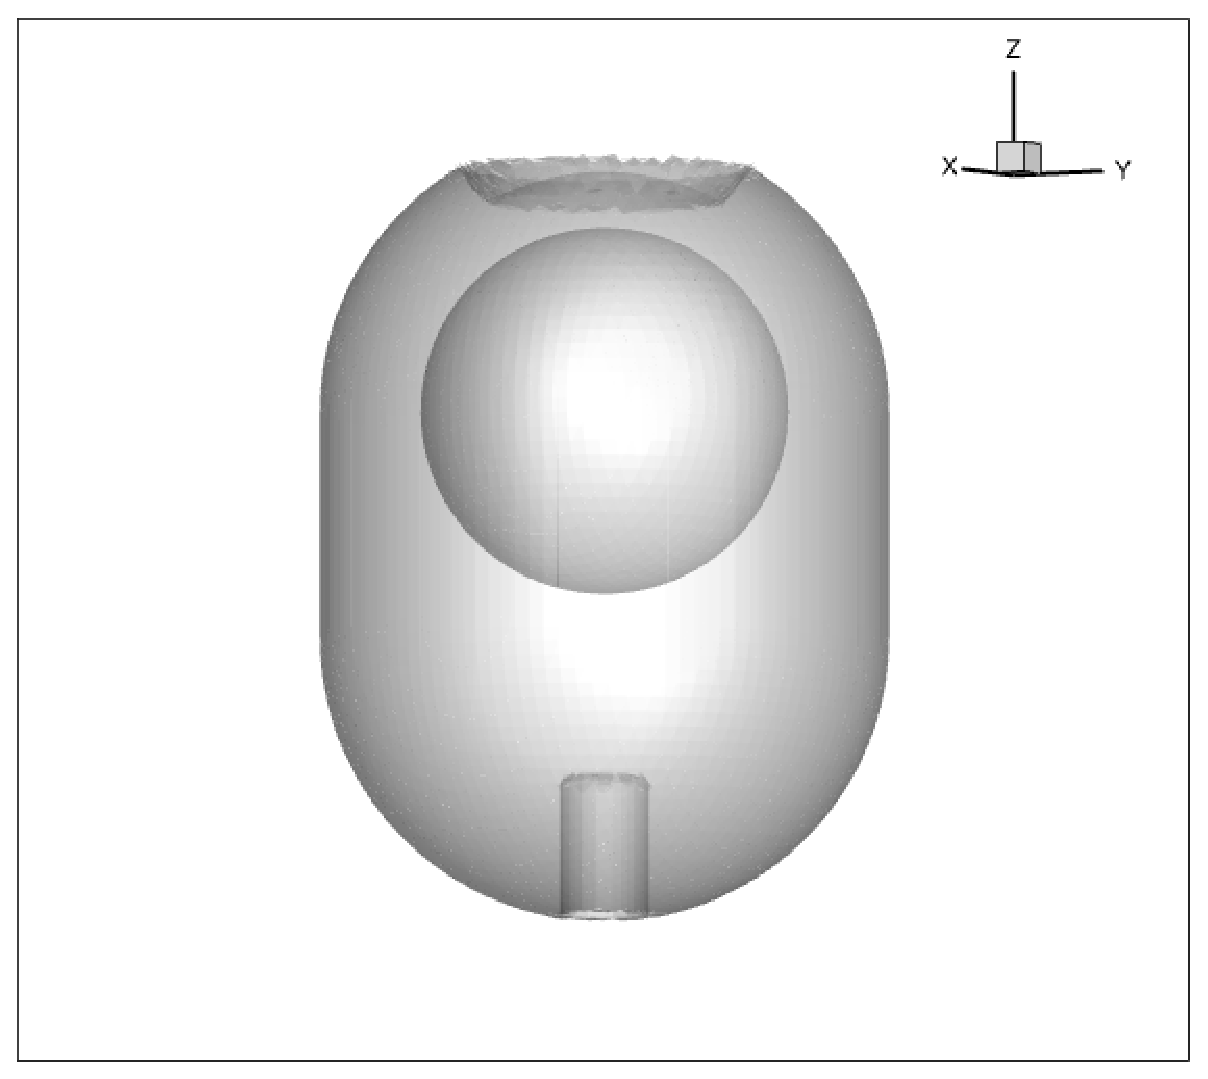
\includegraphics[width=0.3\textwidth]{3D_WEJ4p875_0.eps} 
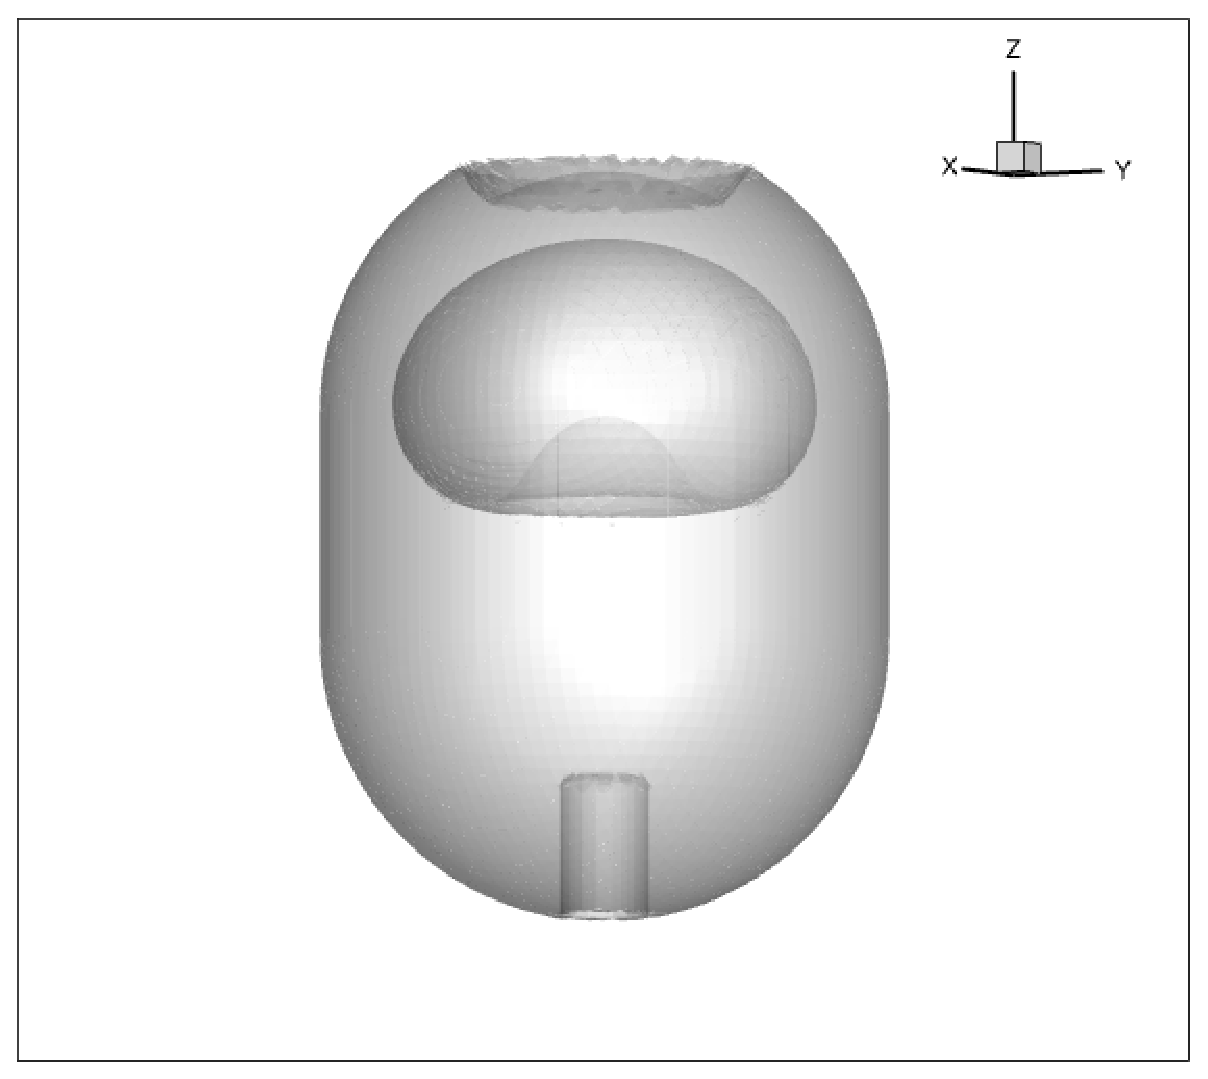
\includegraphics[width=0.3\textwidth]{3D_WEJ4p875_400.eps} 
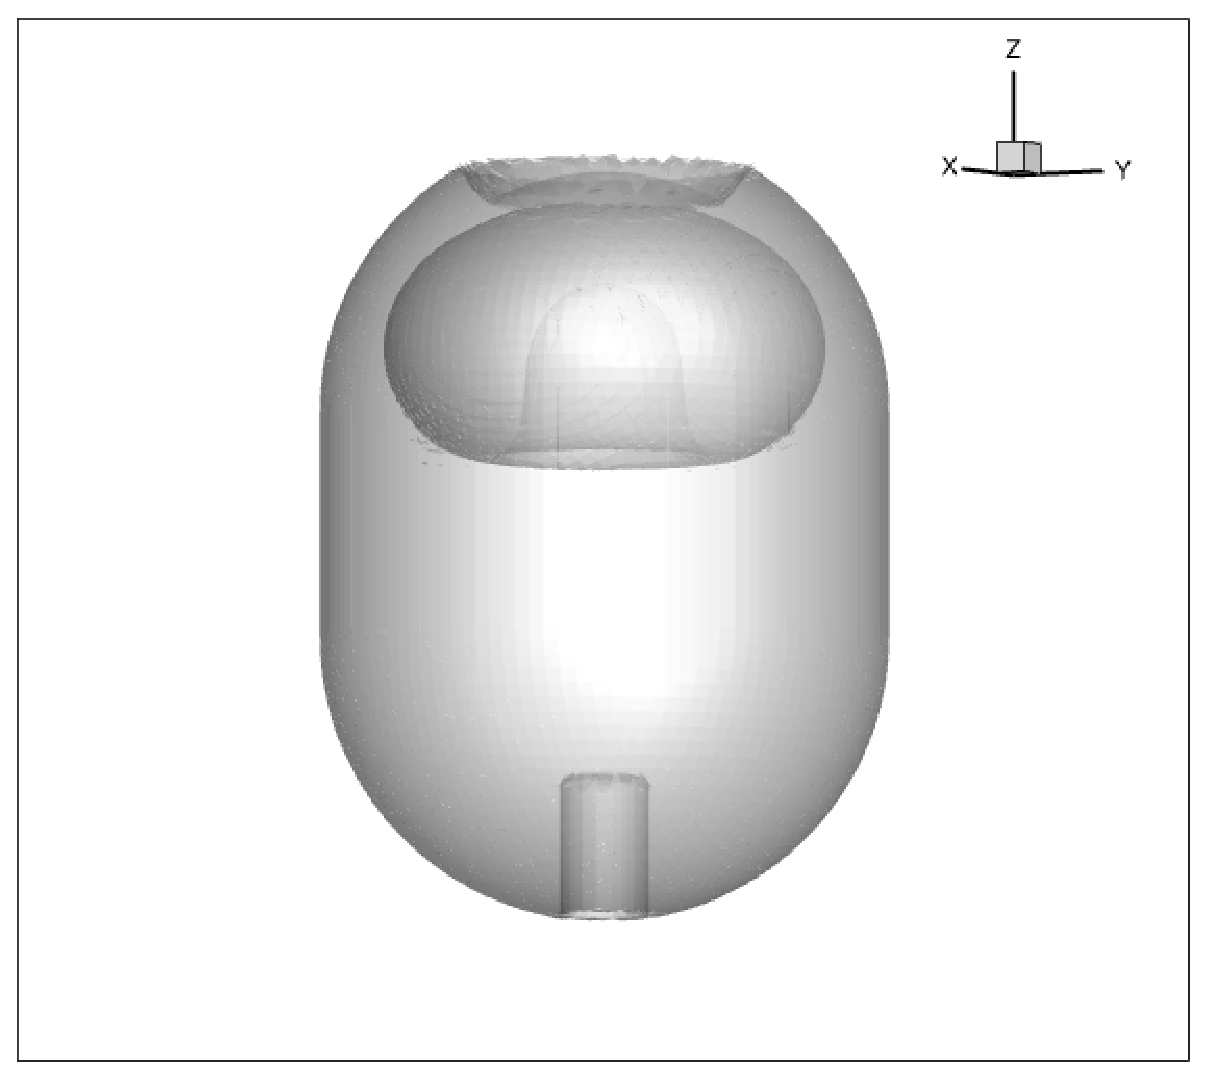
\includegraphics[width=0.3\textwidth]{3D_WEJ4p875_800.eps} 

\caption{The deformation of a ``spherical ullage'' due to a liquid jet.  
	$We_{j}=4.875$.  
	Times=$0.0$, $8.45$, and $15.7$.
	The jet does not penetrate the ullage in this
	case.  The computational grid size was $64\times 64\times 64$. }
 \label{3DWEJ4p875}
\end{figure}

\begin{figure}[htbp]
\centering

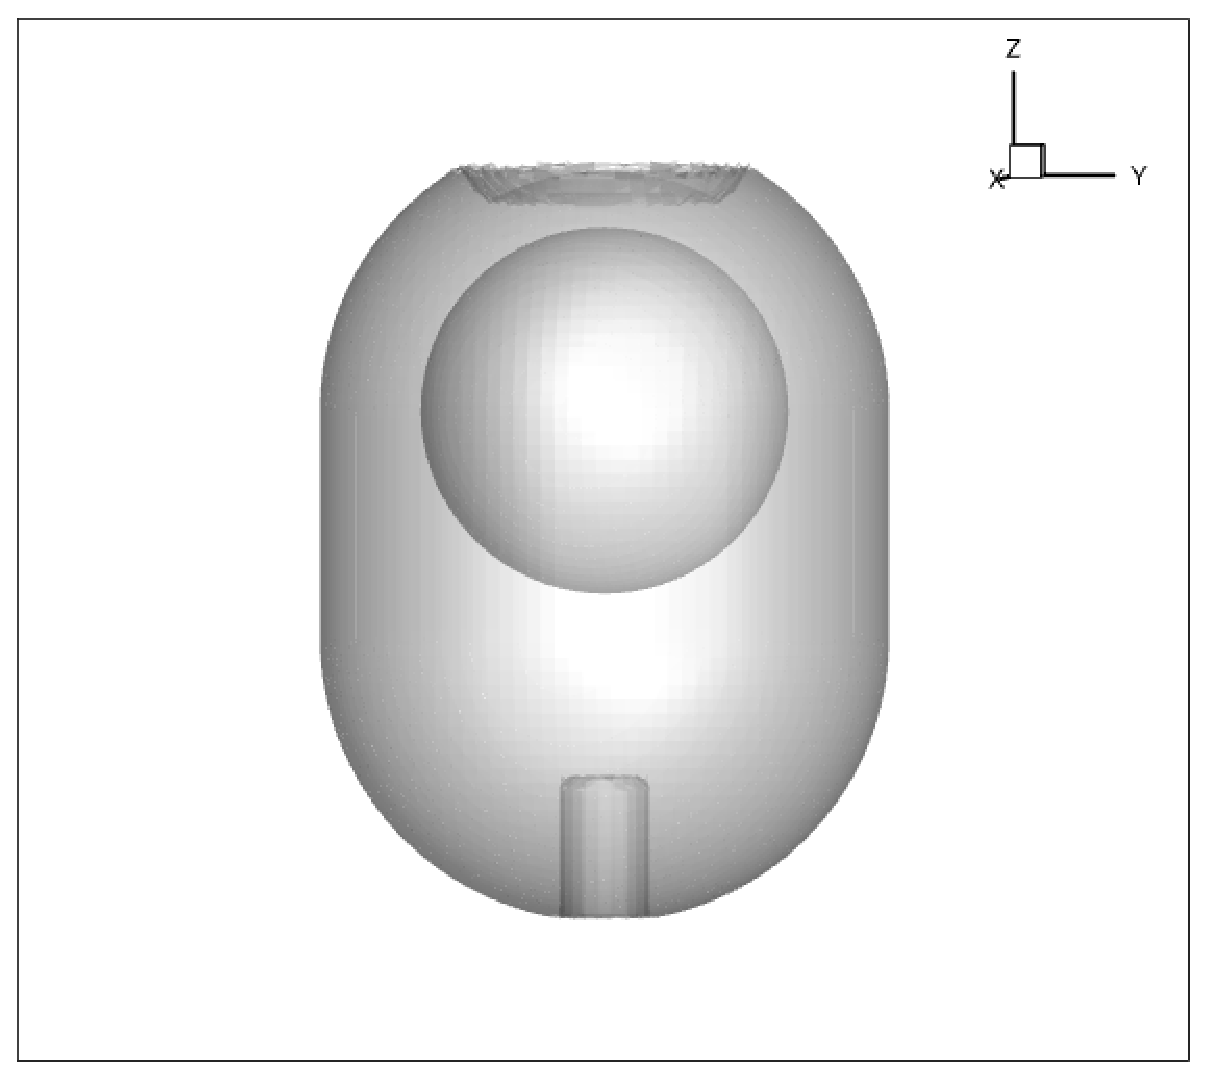
\includegraphics[width=0.3\textwidth]{3D_WEJ5p25_0.eps} 
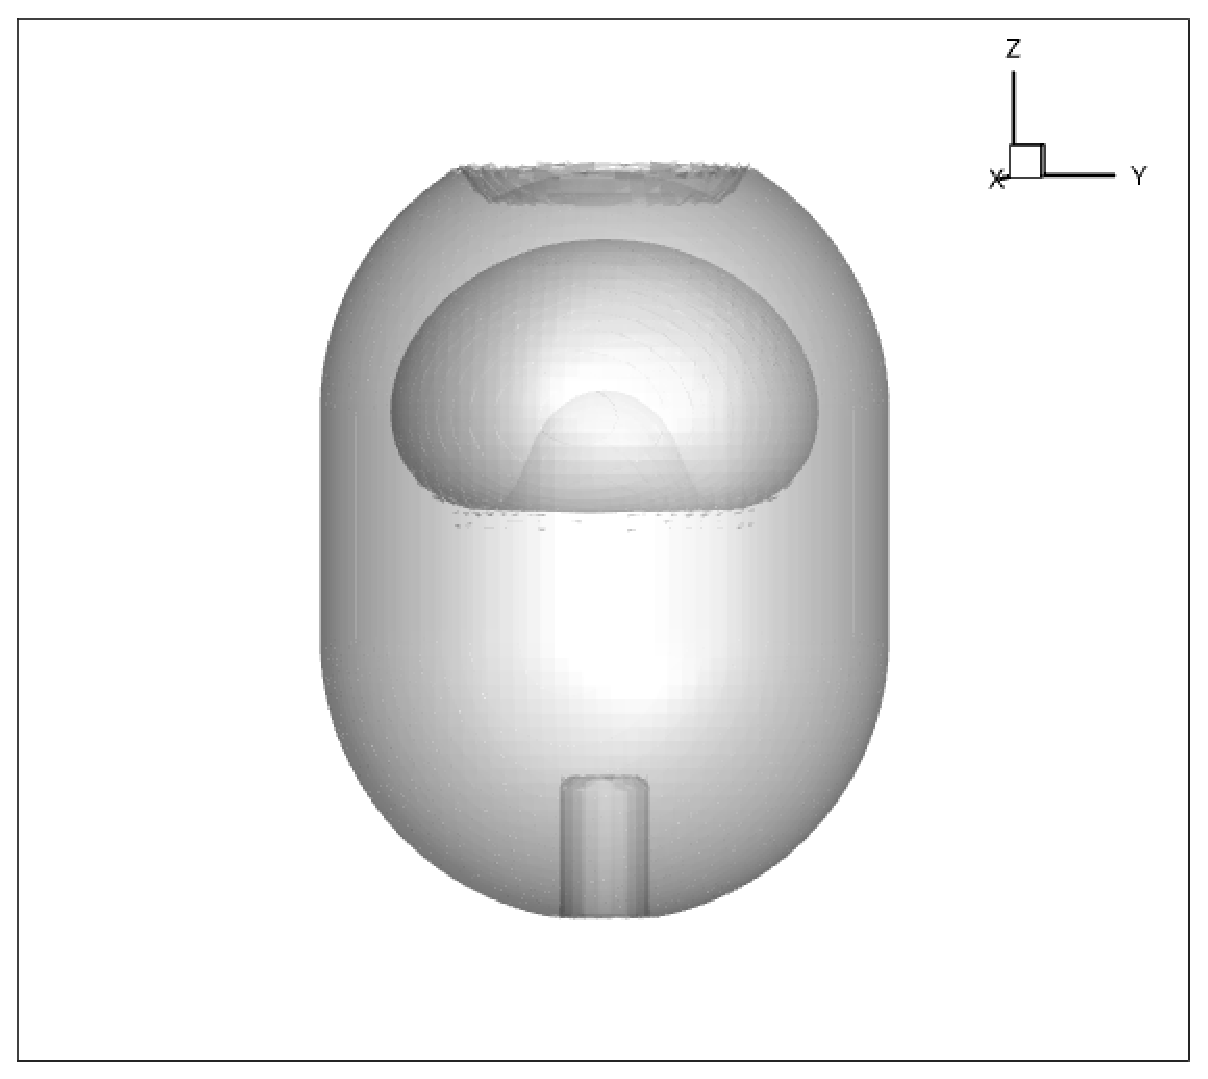
\includegraphics[width=0.3\textwidth]{3D_WEJ5p25_400.eps} 
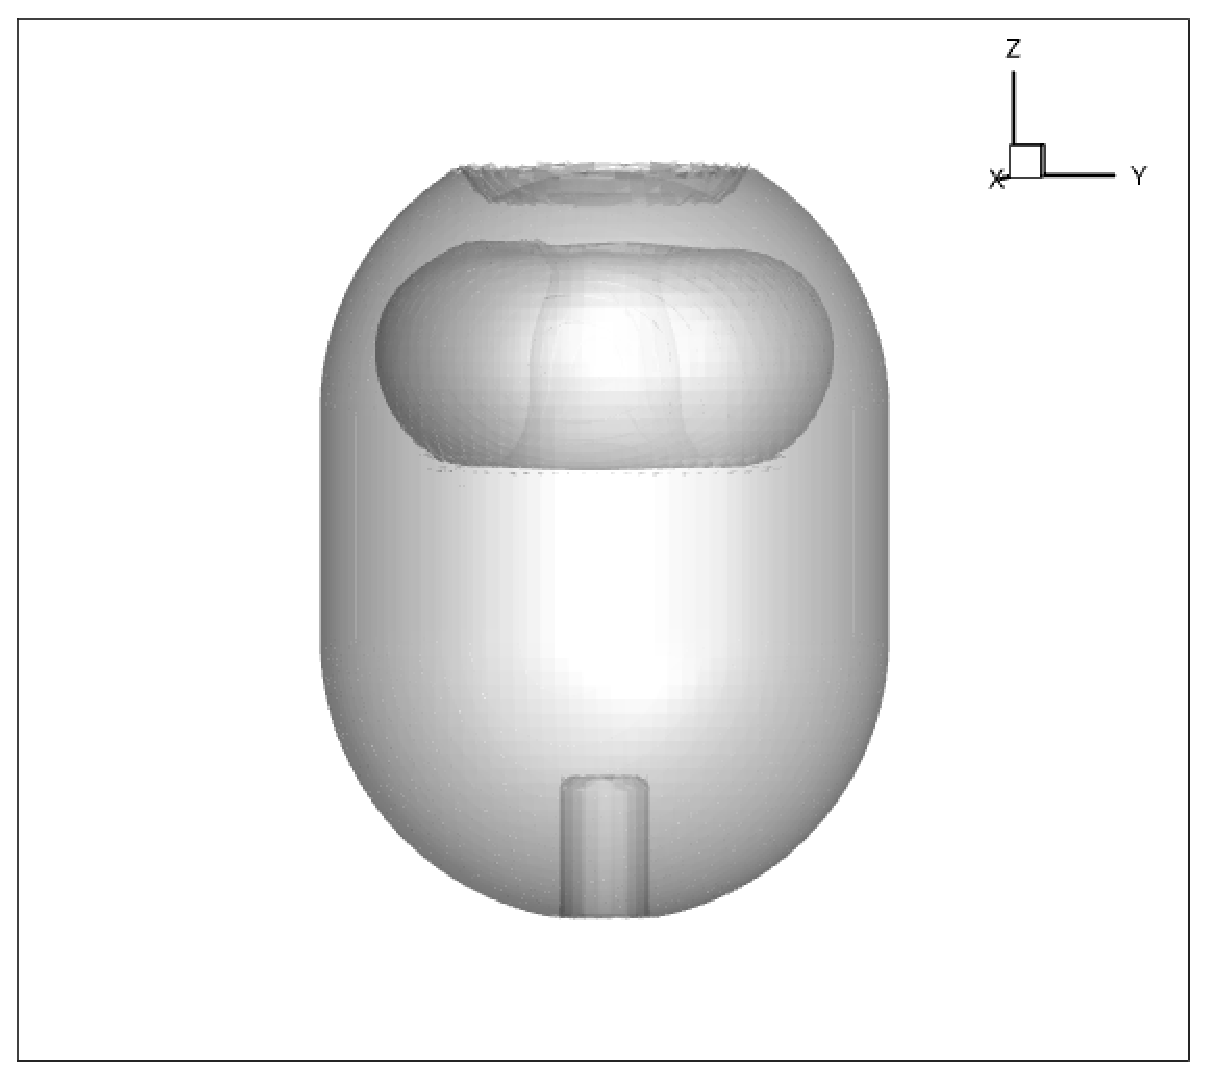
\includegraphics[width=0.3\textwidth]{3D_WEJ5p25_800.eps} 

\caption{The deformation of a ``spherical ullage'' due to a liquid jet.  
	$We_{j}=5.25$. 
	Times=$0.0$, $7.84$, and $15.5$.
	The jet penetrates the ullage in this
	case.  The computational grid size was $64\times 64\times 64$. }
 \label{3DWEJ5p25}
\end{figure}


\begin{figure}[htbp]
\centering

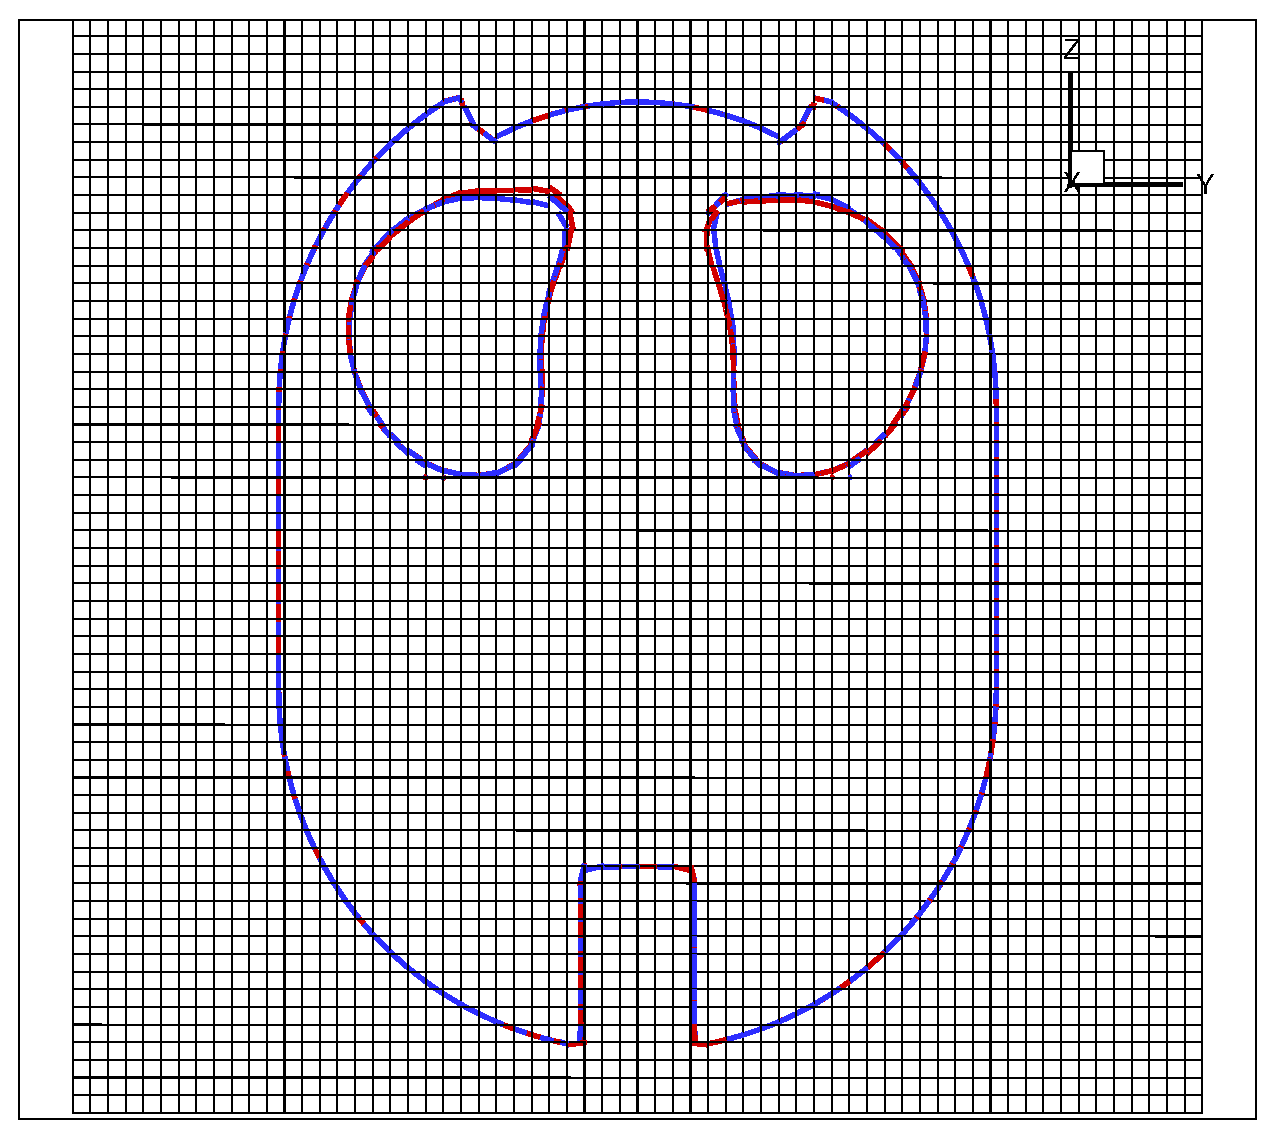
\includegraphics[width=0.8\textwidth]{MLBLUE_VS_GNRED.eps} 

\caption{
Comparison of the vapor-liquid interface just after break-up:
decision tree
machine learning optimization (ML) (blue) versus 
Gauss Newton 
optimization (GN) (Red) ($t=15.5$) 
for the break-up of a ``spherical ullage'' due
to an impinging jet.  }
 \label{ML_VS_GN}
\end{figure}


\section{Conclusions}

In this article the following results were reported for the
first time:
\begin{itemize}
	\item The Continuous MOF (CMOF) method will compute multiphase
		flow results which are more physically realistic and
		convergent under grid refinement than results computed
		using the MOF method.  This property of CMOF takes place
		when surface tension and viscosity forces are non-negligible.
		We refer the reader to section \ref{bubform} 
		(bubble formation, comparison with 
		experiments\cite{helsby1955behaviour}),
		section \ref{liqlens} (Liquid Lens, added noise),
		section \ref{freezing_sec}
		(freezing of a water drop, comparison with 
		experiments\cite{hu2010icing} and convergence study
		(Figure \ref{freezing_conv_study})), and
		section \ref{TPCEsec} (impingement of liquid jet on a
		gas bubble, comparison with experiments 
		\cite{bentz1992jet}).
	\item Our new Decision Tree machine learning algorithm 
		significantly reduces the CPU time to reconstruct
		the CMOF interface slopes with negligible
		effects on the simulation results; see Tables
		\ref{zalesaktable}, \ref{zalesakcost}, and
		\ref{3DCOST}.
	\item Our new added mass algorithm described in 
		section \ref{addmass_sec} reduced the cost of 
		our freezing simulations 
		(section \ref{freezing_sec}) by a factor of 100 without
		sacrificing agreement with experiments.
\end{itemize}

%%SUSSMAN REVISION
In the future, we plan to compare and contrast the present directionally split
conservative method with a much faster unsplit, non-conservative method.
The directionally split method requires 3 sweeps through the grid in 3D which
makes the advection step (Equations (\ref{advection}) through
(\ref{eq:transport})) the bottleneck in our
numerical algorithm.

\section{Conflict of interest statement }

On behalf of all authors, the corresponding author states that there is no conflict of interest.

%%\biboptions{sort&compress}
\bibliography{cmof_paper}

\end{document}
%%% Local Variables:
%%% mode: latex
%%% TeX-master: t
%%% End:
